\documentclass{cslthse-msc}
\usepackage[utf8]{inputenc}
\usepackage[english]{babel}
\usepackage{amsmath}
\usepackage{amsfonts}
\usepackage{amssymb}
\usepackage{amsthm}
%\usepackage{makeidx}
\usepackage{graphicx}
\usepackage{microtype}
\usepackage{algorithm, algorithmicx}
\usepackage{algpseudocode}
\usepackage[titletoc, header, page]{appendix}
\usepackage{hyperref}
\usepackage{cleveref}
\usepackage{cite}


\crefname{app}{Appendix}{Appendices}
\crefname{procedure}{Algorithm}{Procedure}


\newtheorem{definition}{Definition}[chapter]
\setcounter{secnumdepth}{3}
\setcounter{tocdepth}{2}

\renewcommand{\algorithmicrequire}{\textbf{Precondition:}}
\renewcommand{\algorithmicensure}{\textbf{Input:}}

\floatstyle{ruled}
\newfloat{function}{htbp}{lok}
\floatname{function}{Function}

\crefname{function}{function}{functions}
\Crefname{function}{Function}{Functions}


\algdef{SE}[DOWHILE]{Do}{doWhile}{\algorithmicdo}[1]{\algorithmicwhile\ #1}%

\author{
	Philip Ståhl \\
	{\normalsize \href{mailto:ada10pst@student.lu.se}{\texttt{ada10pst@student.lu.se}}}
	\and
	Jonatan Broberg \\
    {\normalsize \href{mailto:elt11jbr@student.lu.se}{\texttt{elt11jbr@student.lu.se}}}
}

\title{Dynamic Fault-Tolerance and Task Scheduling in Distributed Systems}
\subtitle{}
\company{Mobile and Pervasive Computing Institute (MAPCI), Lund University}
\supervisors{Björn Landfeldt, \href{mailto:bjorn.landfeldt@eit.lth.se}{\texttt{bjorn.landfeldt@eit.lth.se}}}{}
\examiner{Christian Nyberg, \href{mailto:christian.nyberg@eit.lth.se}{\texttt{christian.nyberg@eit.lth.se}}}

\date{\today}
%\date{January 16, 2015}

\acknowledgements{
We would like to thank our supervisor Björn Landfeldt and MAPCI for there input.

Maybe also:
Shubhabatra, Ericsson, Jörn, Doan, examiner Christian Nyberg. (Or simply all the people at Mapci)

%If you want to thank people, do it here, on a separate right-hand page. Both the U.S. \textit{acknowledgments} and the British \textit{acknowledgements} spellings are acceptable.
}

\theabstract{
This document describes the Master's Thesis format for the theses carried out at the Department of Computer Science, Lund University. 

%Your abstract should capture, in English, the whole thesis with focus on the problem and solution in 150 words. It should be placed on a separate right-hand page, with an additional \textit{1cm} margin on both left and right. Avoid acronyms, footnotes, and references in the abstract if possible.

%Leave a \textit{2cm} vertical space after the abstract and provide a few keywords relevant for your report. Use five to six words, of which at most two should be from the title.

}

\keywords{reliability, distributed computing, dynamic fault-tolerance, task scheduling, Poisson}

%% Only used to display font sizes
\makeatletter
\newcommand\thefontsize[1]{{#1 \f@size pt\par}}
\makeatother
%%%%%%%%%%


\begin{document}
\makefrontmatter

\chapter{Introduction} \label{ch:introduction} 
\section{Background and Motivation} \label{sec:introduction_backgroud_motivation}
Ensuring a predefined level of reliability is of major concern for many cloud service providers. Cloud computing is growing rapidly, and users demand more services and higher availability and reliability. Therefore, providing fault tolerant systems and improving reliability by more sophisticated task scheduling algorithms has become very important and gained a lot of research interest.

Cloud systems often consists of heterogeneous hardware and any of the, often vast number of, components may fail at any time. Consequently, as computational work is distributed across multiple resources, the overall reliability of the application decreases. To cope with this issue, a fault-tolerant design or error handling mechanism needs to be in place. Ensuring reliability raises complexity to the resource allocation decisions and fault-tolerance mechanisms in highly dynamic distributed systems. For cloud service providers, it is necessary that this increased complexity is taken care of without putting extra burden on the user. The system should therefore ensure these properties in a seamless way.

In some cases, vendors, such as carrier providers, are obliged by law to achieve a specific level of availability or reliability. In such cases, quality aspects such as latency and resource usage may need to be sacrificed to reach the required level. By using static and dynamic analysis of the infrastructure and the mean-time-between-failure for the available resources, a statistical model can be created to verify that the required level is reached. However, due to the dynamic properties of distributed environments, such a model must also be dynamic. 

Furthermore, reliability is of particular importance for long running applications or services when a certain level of reliability is required. Despite fulfilling the required level at the time of deployment, as the state of the system changes, the required reliability may no longer be fulfilled, and actions must be taken to still reach the required level.

One way of increasing the reliability is by replicating application tasks, i.e. creating identical copies. Having identical copies, also called replicas, results in increased redundancy, and allows for continued execution of the application, despite the event of failure of a task copy. Seamlessly being able to continue the execution or computations performed, without losing any data is of particular interest in data stream processing.

A drawback of replication is the extra resources needed. If replicating a task \emph{n} times with every replica performing the same computation on the same input, $n$ times as many resources are needed, hence a lot of computational resources is wasted. Dynamic analysis of the system and an adaptive scheduling technique could help in determining on which resources replicas should be placed for optimal resource usage and load balancing.

%TODO lång mening?
In this master thesis, a dynamic fault-tolerant model is presented, which ensures the required reliability is met by replicating tasks, and doing so in an optimal way by dynamically adapting to changing properties of the system and available resources.

\section{Related work} \label{sec:introduction_related_work}
The interest in reliability for distributed systems has gained increased attention recently~\cite{replicationManagement}. Due to the heterogeneous resources composing distributed environments such as cloud and grid systems, ensuring reliability is a complex task~\cite{cloudServiceRel, surveyReliabilityDistr}.

A lot of scheduling techniques have been designed, aiming at maximizing reliability of computational jobs in distributed environments under various constraints such as meeting task deadlines or minimizing execution time~\cite{algoOptTimeMaxRel, optTaskAllocationForMaxRel, taskAllocation, taskAllocationSwarm, algoMaxRelEndToEndConstraint, algoMinExTime, schedReplicas}. Maximizing reliability for these algorithms are a secondary concern, while meeting the constraints is the primary. Other algorithms have been developed which focus on increasing the reliability~\cite{optResourceAllMaxPerformance, matchSchedAlgoMinFailure}, and some have increased reliability as the primary objective~\cite{safetyRelTaskAllocation, improvedTaskAllMaxRel}. Common for these scheduling techniques is that while they try to maximize reliability, they do not ensure a certain level of reliability is met. Furthermore, the algorithms are usually static in the way that they do not account for the dynamic behavior of distributed systems. In addition, they make assumptions such as known execution times of tasks, which makes them unsuitable for long running applications or services without a known execution time.

A lot of work has been done in the area of designing fault-tolerant systems by using checkpoint/restart techniques [TODO]. %TODO add reference
These techniques relies of the notion of a stable storage, such as a hard-drive, which is persistent even in the case of a system failure. Checkpoint techniques are usually employed for applications or jobs where the computations done take a very long time [TODO].

Some previous attempts at designing fault-tolerant systems by the use of replication has been made~\cite{designFaultTolerantSched, evalReplicationSched, taskSchedulingReplication, effTaskReplMobGrid, relGridServicePredConstraint}. In \cite{evalReplicationSched}, a static number of replicas is used for every application being deployed. Furthermore, they do not guarantee that all replicas are deployed, instead they use a best-effort approach, where replicas are deployed only if resources are available. In contrast to~\cite{evalReplicationSched}, \cite{ effTaskReplMobGrid, taskSchedulingReplication, designFaultTolerantSched} dynamically determines the number of replicas based on the state of the system. However, they are all static in that failed replicas are not restarted, and do therefore not ensure the reliability is met over time. Furthermore, while~\cite{designFaultTolerantSched} dynamically determines the number of replicas to use, the scheduling decision on which resources to put the replicas is done after the number of replicas has been determined. As the reliability vary between resources in a heterogeneous environment, the number of replicas needed depends on which resources are used. Therefore, determining the number of replicas needed and where to place then should be a joint process.

A quite old but still relevant work is found in~\cite{dynAdaptRepl} in which a framework for dynamically replicating tasks in a multi-agent system is presented. The authors introduce a software architecture which can act as support for building reliable multi-agent systems. Since the available resources often are limited, they say that it is not feasible to replicate all components. Therefore, they introduce the concept of a criticality for each agent, which is allowed to evolve during runtime. An agent's criticality is calculated using the CPU usage and communication activity of the agent, and is used to determine the number of replicas needed, along with a predefined minimum number of replicas. The proposed solution also allows for dynamically adapting the number of replicas and the replication strategy itself (passive/active). %TODO Do they meet a desrided level of reliablity?

Other approaches to improve reliability in Multi-Agent Systems (MAS) by the use of replication is presented in~\cite{replicatingAgents, adaptiveMASReplication, adaptiveAgentReplication}. While being adaptive to system state, the solution presented in~\cite{replicatingAgents} still faces the problem of having a single point of failure due to a communication proxy. This problem is avoided in~\cite{adaptiveMASReplication}, where a decentralized solution is proposed, and where the number of replicas and their placement depends on the system state. However, instead of ensuring a given level of reliability is met, they aim at maximizing the reliability and availability based on available resources. %TODO check this again

A dynamic and adaptive algorithm, which dynamically varies the number of replicas depending on system load is presented in~\cite{adaptiveCheckPointAndRep}. The proposed algorithm does not ensure a certain reliability. Instead, it reduces the number of replicas during peak hours, in order to reduce system load. Since the reliability of system decreases during higher load~\cite{studyOfFailures, implicationsOfFailures}, the number of replicas should be increased instead of decreased in order to stay above the required level of reliability.

A fault-tolerant scheduling technique incorporating a replication scheme is presented in~\cite{faultTolerantSchedPolicy}. While being dynamic in that failed replicas are restarted, it is static in that the user defines the number of replicas to use, hence it does not ensure a specific level of reliability is met.

The techniques used in~\cite{selfAdaptRel, dynAdaptRepl, relModelWebServices} are more dynamic and adaptive to the dynamic behaviour of distributed systems. However, reliability is defined as producing the correct result, and achieved by techniques like majority voting and \emph{k-modular redundancy}. An adaptive approach, which adapts to changes in the execution environment is presented in~\cite{imprRelAdaptRL}. In it, they present an adaptive scheduling model based on reinforcement learning, aiming at increasing the reliability. However, they assume that a task's profile, including execution time, is available.

\section{Our contributions} \label{sec:introduction_contributions}
To our knowledge, no previous attempt has been made which in a fully dynamic manner ensures a certain level of reliability for long running applications or services. Some previous work dynamically calculates the number of replicas, but are static in that failed replicas are not restarted, while others use a static number of replicas, and dynamically restart failed ones.

We propose a framework which ensures a user determined level of reliability by the use of replication. Furthermore, the method ensures a minimized use of resources by not using more replicas than needed. This is achieved by scheduling replicas on the most reliable resources first and foremost. Finally, the system is periodically monitored in order to adapt to changing system properties.

The framework is not limited to a specific type of distributed environment, nor the reliability model used. The reliability model and scheduling algorithm is easily replaced to consider more parameters, or to include load-balancing.

%TODO
%Finally, our solution is fully distributed and thereby avoids having a single point of failure, which may be the case in grid environments with a single Resource Management System. (THIS CONTRADICTS NOT BEING LIMITED TO A SPECIFIC DISTRIBUTED ENVIRONMENT)

Our model is implemented using the actor-based application environment \emph{Calvin} \cite{calvin}, developed by Ericsson. While \emph{Calvin} is mainly an environment for Internet of Things (IoT) applications, it suites our purpose well. The model is evaluated by running a set of experiments in a small cluster. %TODO

The report is structured as follows: in \cref{ch:background} all necessary background theory is provided, in \cref{ch:design} we present our model and contribution in more detail, \cref{ch:evaluation} presents an evaluation of our solution and in \cref{ch:discussion} the solution is discussed. \Cref{ch:future_work} presents future work and \cref{ch:conclusions} concludes the report. 

\section{Goal} \label{sec:introduction_goals}
The goal of this thesis is to devise a method for dynamically ensuring a certain level of reliability for distributed applications or services. Reliability will be achieved by replicating tasks.

First, a reliability model will be designed, describing the reliability of the available resources, and for applications using these resources.

Secondly, a framework will be designed which will automatically detect node failures and based on the reliability of the available resources creates enough replicas to reach the required reliability level.

Lastly, the system and its running applications will be periodically monitored in order to adapt the resources' reliability and the number of replicas needed as the properties of the system varies over time.

The model will be implemented and tested using the IoT application framework \emph{Calvin}.

\chapter{Background} \label{ch:background}
In this chapter we provide all the necessary background theory to fully understand the rest of the report.
\section{Computational Environment} \label{sec:background_comp_env}
The computational environment used in this thesis is distributed computing, i.e. several resources working together towards a common goal.

\subsection{Types of distributed computing} \label{subsec:background_types_of_distr_comp}
Distributed computing systems (DCS) are composed of a number of components or subsystems interconnected via an arbitrary communication network~\cite{relModelDistSimSystem, efficientRelAnalysisAlgo}. There are a number of different types of distributed environments, e.g. grids, clusters, clouds and heterogeneous distributed computing systems.

\subsubsection{Grid computing}
A grid is a collection of autonomous resources that are distributed geographically and across several administrative domains, and work together to achieve a common goal, i.e. to solve a single task~\cite{compStudyLoadAndCloud, relAndPerfGridServices, evalOfGridRel}.

Each domain in a grid usually has a centralized scheduling service called Resource Management System (RMS) which accepts job execution requests and sends the job's tasks to the different resources for execution~\cite{evalOfGridRel}.

The reliability of the cloud computing is very critical but hard to analyze due to its characteristics of massive-scale service sharing, wide-area network, heterogeneous software/hardware components and complicated interactions among them~\cite{cloudServiceRel}.

%COPIED:The grid computing system has emerged as an important new field, distinguished from conventional distributed computing systems by its focus on large-scale resource sharing, innovative applications, and, in some cases, high performance orientation. \cite{hierarchicalRelModeling}.

\subsubsection{Cluster}
A cluster system is usually a number of identical units managed by a central manager. It is similar to a grid, but differ in that resources are geographically located at the same place. The resources work in parallel under supervision of a single administrative domain. From the outside it looks like a single computing resource~\cite{compStudyLoadAndCloud}.

\subsubsection{Cloud}
A cloud has been described as the next generation of grids and clusters. While it is similar to grids and clusters, the main difference is that cloud has multiple domains~\cite{compStudyLoadAndCloud}. Resources can be geographically distributed, and software and hardware components are often heterogeneous, and therefore analyzing and predicting workload and reliability is usually very challenging~\cite{surveyReliabilityDistr}. 

%COPIED: "Cloud computing is a style of computing where service is provided across the Internet using different models and layers of abstraction [4]. It refers to the applications delivered as services [5] to the mass, " \cite{faultToleranceChallenges}

%COPIED: Cloud computing is different from but related with grid computing, utility computing and transparent computing. Grid computing [1] is a form of distributed computing whereby a "super and virtual computer" composed of a cluster of networked, loosely-coupled computers acts in concert to perform very large tasks.”

\subsubsection{Heterogeneous distributed computing systems}
Heterogeneous Distributed Computing Systems, HDCS, is a system of numerous high-performance machines connected in a high-speed network. Therefore, high-speed processing of computational heavy applications is possible~\cite{algoMinExTime}. %TODO add info

The majority of distributed service systems can be viewed as CHDS, (Centralized Heterogeneous Distributed System). A CHDS consists of heterogeneous sub-systems which are managed by a centralized control center. The sub-systems have various operating platforms and are connected in diverse topological networks~\cite{studyServiceRel}.

%COPIED: Most of the distributed service systems can be modeled as a CHDS. This type of distributed systems consists of heterogeneous sub-systems with various operating platforms on different computers in diverse topological networks, which are managed by a control center. The heterogeneous sub-distributed systems are composed of different types of computers with various operating systems connected by diverse topologies of networks. These sub-systems exchange data with virtual machine through system service provider interface. They are connected with virtual nodes by routers \cite{studyServiceRel}.

\subsection{Dynamic versus static environments} \label{subsec:background_dyn_stat_env}
A distributed computing environment can be either static or dynamic.

In a static environment, only homogenous resources are usually installed~\cite{compStudyLoadAndCloud}. Prior knowledge of node capacity, processing power, memory, performance and statistics of user requirements are required. Changes in load during run time is not taken into account which makes environment easy to simulate but not well suited for heterogeneous resources. Once the system has been put into place, resources are neither added nor removed from the system.

In contrast to static environments, a dynamic environment usually consists of heterogeneous resources~\cite{compStudyLoadAndCloud}. Once the system has been put into place, resources can be dynamically added or removed. In such environments, prior knowledge is therefore not about enough, since the requirements of the user and the available resources can change during runtime. Runtime statistics is therefore usually collected and taken into account. Dynamic environments are difficult to simulate, algorithms exist which easily adopt to runtime changes. 


\section{Faults in distributed environments} \label{sec:background_faults_distr_env}
In distributed environments, a larger number of faults can occur due to its complexity. Therefore, when modeling faults and reliability in such environments, a fault model is usually employed, describing what kind of faults are being considered.

\subsection{Types of Faults} \label{subsec:background_types_of_faults}
A fault is usually used to describe a defect at the lowest level of abstraction~\cite{faultTolerantFundamentals}. A fault may cause an error which in turn may lead to a failure, which is when a system has not behaved according to its specification.

In distributed environments, especially with heterogeneous commodity hardware, several types of failures can take place, which may affect the running applications. Such failures include, but are not limited to, overflow failure, timeout failure, resource missing failure, network failure, hardware failure, software failure, and database failure~\cite{cloudServiceRel}. Failures are usually considered to be either~\cite{evalOfGridRel}:

\begin{itemize}
	\item Job related, or
	\item System related, or
	\item Network related.
\end{itemize}

In~\cite{studyOfFailures}, almost ten years of real-world failure data of 22 high performance computing systems was studied and concluded hardware failures to be the single most common type of failure, ranging from 30 to more than 70 percent depending on hardware type, while 10 to 20 percent of the failures were software failures.

\iffalse
%TODO not important?
The possible errors in a Grid environment can be divided into the following three categorize~\cite{effTaskReplMobGrid}:
\begin{itemize}
	\item Crash failure - When a correctly working server comes to a halt.
	\item Omission failure - When a server fails to respond to incoming requests and to send messages
	\item Timing failure - When a server responds correctly but beyond the specified time interval
\end{itemize}
\fi

\subsection{Fault models} \label{subsec:background_fault_models}
When studying the reliability of distributed systems or the reliability of applications running in distributed computing environments, one usually starts with specifying which fault model is used, and the model developed is then proved with respect to this fault model~\cite{faultTolerantFundamentals}. In the fault models described in this section, a computational resource is referred to as a node.

\subsubsection{Byzantine fault model} \label{subsub:background_byzantine}
The Byzantine fault model allows nodes to continue interaction after failure. Correctly functioning nodes cannot automatically detect if a failure has occurred and even if it was known that a failure occurred, they cannot detect which nodes have failed. 

Furthermore, the systems behaviour can be inconsistent and arbitrary~\cite{surveyFaultParallel}. Nodes can fail (become Byzantine) at any point of time and stop being Byzantine at any time. A Byzantine node can send no response at all, or it can send an incorrect result. All Byzantine nodes might send the same incorrect result, thereby making it hard to identify malicious nodes~\cite{selfAdaptRel}. %Kan man detektera malicious nodes? 
The Byzantine fault model is very broad since it allows failed nodes to continue interacting, but it is therefore also very difficult to simulate and to analyze.

% COPIED: in which processors may behave in arbitrary, even malevolent, ways). System correctness was always proved with respect to a specific fault model \cite{faultTolerantFundamentals}

\subsubsection{Fail-stop fault model} \label{subsub:background_fail_stop}
The fail-stop model, also called the crash-stop model, is in comparison to the Byzantine fault model much simpler. When a node fails it stops producing any output and stops interacting with the other nodes~\cite{faultTolerantFundamentals}. This allows for the rest of the system to automatically detect when a node has failed. Due to its simplicity, it does not handle subtle failures such as memory corruption but rather failures such as a system crash or if the system hangs~\cite{surveyFaultParallel}. %The fail-stop model has been criticized for not representing enough real-world failures. LAST SENTENCE NEEDED?

%COPIED: This failure model has the practical implication that avoids the use of complicated software and/or hardware replication systems for recovering tasks from failed server. Consequently, the application cannot be successfully serviced by the system if at least one task remains unprocessed at a failed server. \cite{perfRelNonMarkovian}

\subsubsection{Crash-failure fault model}
The crash failure model is quite alike the fail-stop model with the difference that nodes do not automatically detect the failure of a node~\cite{faultTolerantFundamentals, adaptiveAgentReplication}.

\subsubsection{Fail-stutter fault model}
%TODO Ta bort? Verkar knappt används och finns inte mycket information om den
Since the Byzantine model is very broad and complicated and the fail-stop model doesn't represent enough real-world failures, a third middle ground model has been developed. It is an extension of the fail-stop model but differ in that it also allows for performance fault, such as unexpectedly low performance of a node~\cite{surveyFaultParallel}.

\subsection{Failure distribution} \label{subsec:background_failure_distribution}
Models describing the nature of failures in distributed computing environments, are usually based on certain assumptions, and are usually only valid under those assumptions. Commonly made assumptions about failures and the computational environment are \cite{relModelDistSimSystem, relModelAnalysis, cloudServiceRel, studyServiceRel, hierarchicalRelModeling, selfAdaptRel}:
\begin{itemize}
	\item Each component in the system has only two states: \emph{operational} or \emph{failed}
	\item Failures of components are statistically independent
	\item Components have a constant failure rate, i.e. the failure of a component follows a Poisson process
	\item Fully reliable network
\end{itemize}

When modelling reliability for grid systems, it is common to also assume a fully reliable Resource Management System (RMS)~\cite{relAndPerfGridServices, relGridServicePredConstraint}, which is a non-negligible assumption since the RMS is a single point of failure.

%TODO definera "failures", vilka brukar inkluderas?
%When modelling system reliability, failures are usually assumed to follow a Poisson process with a constant failure rate~\cite{algoMaxRelEndToEndConstraint} \cite{algoMinExTime} \cite{relModelDistSimSystem} \cite{optTaskAllocationForMaxRel} \cite{perfImplPerCheckPoint} \cite{optCheckpointInterval} \cite{realTimeSchedAlgo}. For such a model to be valid, it is assumed that failures between resources are statistically independent with a constant failure rate~\cite{algoMaxRelEndToEndConstraint}. %we use Poisson and have a non-constant failure rate?

Constant failure rates are not likely to model the actual failure scenario of a dynamic heterogeneous distributed system~\cite{algoMinExTime}. The failure rate for a hardware component usually follows a bathtub shaped curve~\cite{surveyReliabilityDistr}. The failure rate is usually higher in the beginning due to that the probability that a manufacture failure would affect the system is higher in the beginning of the systems lifetime. After a certain time the failure rate drops and later increases again due to that the component gets worn out. %TODO refer to this in design.

Statistically independent failures is also not very likely to reflect the real dynamic behaviour of distributed systems~\cite{surveyReliabilityDistr, cloudServiceRel}. Faults may propagate throughout the system, thereby affecting other components as well~\cite{relGridSystems}. In grid environments, a sub-system may consist of resources using a common gateway to communicate with the rest of the system. In such a scenario, the resources do not use independent links~\cite{optResourceAllMaxPerformance}. As failures are likely to be correlated~\cite{perfImplPerCheckPoint}, the probability of failure increases with the number of resources the job uses.

Other factors also affect the likelihood of resource failures. Several studies have concluded a relationship between failure rate and the load of the system~\cite{studyOfFailures, implicationsOfFailures}. Furthermore, \cite{studyOfFailures, implicationsOfFailures} also show that failures are more likely to occur during daytime than at night, which may be a consequence of the system load being higher during daytime. In addition, components which have failed in the past are more likely to fail again~\cite{implicationsOfFailures}.

While a Poisson process is commonly used to describe failures, \cite{studyOfFailures} shows that failures are better modelled by a Weibull distribution with a shape parameter of 0.7 - 0.8. However, despite not always reflecting the true dynamic failure behaviour of a resource, a Poisson process has been experimentally shown to be reasonable useful in mathematical models~\cite{experimentalFailureAssessment}.

\section{Reliability} \label{sec:background_reliability}
\subsection{Reliability definition} \label{subsec:background_reliability_definition}
Reliability in the context of software applications can have several meanings, especially for applications running in distributed systems. Often, reliability is defined as the probability that the system can run an entire task successfully~\cite{taskAllocation, relModelDistSimSystem, studyServiceRel, hierarchicalRelModeling, generalAlgoRelEval, realTimeRelAnalysis, selfAdaptRel, perfRelNonMarkovian}. A similar definition, for applications running in distributed environments, is that reliability is the probability of a software application to perform its intended functions for a specified period of time~\cite{surveyReliabilityDistr, surveyRelPrediction, relDistApplications}, and is commonly used for application with time constraints. Finally, reliability can also be defined as the probability that a task produces the correct result~\cite{surveyRelPrediction, relAndPerfGridServices, relGridServicePredConstraint, relModelWebServices, selfAdaptRel}. The latter is usually used together with the Byzantine fault model. 

\iffalse
%Onödig definition??
\cite{surveyReliabilityDistr} defines a software application reliable if the following is achieved:
\begin{itemize}
\item Perform well in specified time $t$ without undergoing halting state
\item Perform exactly the way it is designed
\item Resist various failures and recover in case of any failure that occurs during system execution without proceeding any incorrect result.
\item Successfully run software operation or its intended functions for a specified period of time in a specified environment.
\item Have probability that a functional unit will perform its required function for a specified interval under stated conditions.
\item Have the ability to run correctly even after scaling is done with reference to some aspects.
\end{itemize}
\fi

\subsection{Modelling reliability} \label{subsec:background_modelling_rel}
Reliability of a system highly depends on how the system is used~\cite{surveyRelPrediction}. In order to determine the reliability of a system, one need to take all factors affecting the reliability into account~\cite{surveyReliabilityDistr}. However, including all factors is infeasible. In \cite{factorsAffectingRel}, 32 factors affecting the reliability of software are listed, excluding environmental factors such as hardware and link failure. Other environmental conditions affecting reliability include the amount of data being transmitted, available bandwidth and operation time~\cite{cloudServiceRel, hierarchicalRelModeling}.

For distributed applications, the probability of failure increases since it is dependent on more resources~\cite{relModelDistSimSystem}. Most reliability models are based on the mean time to failure, or the mean time between failures, of resources~\cite{relModelAnalysis}. Conventionally, Mean-Time-To-Failure (MTTF) refers to non-repairable resources, while Mean-Time-Between-Failures (MTBF) refers to repairable objects~\cite{effTaskReplMobGrid}.

\begin{definition} \label{def:mttf}
The Mean-Time-To-Failure for a component is the average time it takes for a component to fail, given that it was operational at time zero.
\end{definition}

\begin{definition} \label{def:MTBF}
The Mean-Time-Between-Failure for a component is the average time between successive failures for that component.
\end{definition}

The MTBF can be calculated as

\begin{equation} \label{eq:MTBF}
MTBF = \frac{total\ time}{number\ of\ failures}
\end{equation}

Assuming failures follow a Poisson process, and using \cref{eq:MTBF}, the reliability for a component can be expressed as 
\begin{equation} \label{eq:resource_reliability}
R(t) = e^{-t/MTBF}
\end{equation}

\Cref{eq:resource_reliability} expresses the probability that a given resource will work for a time $t$. Correspondingly, the probability that a resource will fail during a time $t$ is
\begin{equation} \label{eq:resource_failure_prob}
F(t) = 1- e^{-t/MTBF}
\end{equation}

\iffalse
While redundancy and diversity have been employed as popular methods to attain better reliability [4][5][6][7][8][9][10], they impose extra hardware or software costs.
optimal task allocation. This method does not require additional hardware or software and improves system reliability just by using proper allocation of the tasks among the nodes [8][11][12] [13] [14] \cite{optTaskAllocationForMaxRel}
\\\\
\cite{discContRelModel}
\\\\
System reliability: Due to independence of node and path failures, system reliability can be formulated as: Rs(X) = RS’(X) * Rs” (X) \cite{optTaskAllocationForMaxRel}
\\\\
the reliability model of the sub-distributed systems inherits the traditional models’ characters [19], [20], [21], [22] and has certain limitations. Those traditional models have a common assumption that the operational probabilities of the nodes and links are constant. However, this assumption is unrealistic for the grid, so this assumption was relaxed in [15] by assuming that the failures of nodes and links followed their respective Poisson processes so that their operational probabilities decrease with their working time instead of the constant values 
There are also many other reliability models for software, hardware, or small-scale distributed systems, see, e.g., [14], [23], [24], [25], [26], which cannot be directly implemented for studying grid service reliability. \cite{hierarchicalRelModeling}
\\\\
Reliability evaluation of the hyper-cubes has been addressed recently [7]-[9]. Najjar and Gaudiot have modeled hyper-cube reliability assuming that the system works as long as there is no disconnected working node(s) [7]. This implies that even if a task requirement is satisfied, the system is considered failed whenever there is a disconnected node(s). This reliability is not based on task requirement, but on system managemen. [ A unified task-based dependability model for hyper-cube computers]
\\\\
(the processing element that runs the program under consideration) to some other nodes such that its vertices hold all the needed files for the program under consideration. \cite{relAnalysisFRA}
\\\\
We focus on the study of task allocation decision to achieve maximal distributed system reliability (DSR) under processor resource constraints and total system cost constraint. the task allocation problem has been studied to achieve various goals, such as reliability maximization, safety maximization, fault tolerance increasing, and cost minimization. Their processor reliability was computed from the processor failure rate and the elapsed execution time. As far as we know, the effects of module software reliabilities and module execution frequencies on the optimal task allocation decision have not been studied before. To pursue this topic, we divide the processor reliability into two parts in our system model: the processor hardware reliability and the module software reliability \cite{decisionModelTaskAllocation}
\fi

\section{Fault tolerance techniques} \label{sec:background_fault_tol_tech}
Fault tolerance techniques are used to either predict failures and take an appropriate action before they occur~\cite{faultToleranceChallenges}, or to prepare the system for failures, and take appropriate actions first when they occur. Considering the whole life-span of a software application, fault-tolerant techniques can be divided into four different categories~\cite{surveyReliabilityDistr}:

\begin{enumerate}
\item Fault prevention - elimination of errors before they happen, e.g. during development phase
\item Fault removal - elimination of bugs or faults after repeated testing phases
\item Fault tolerance - provide service complying with the specification in spite of failure
\item Fault forecasting - Predicting or estimating faults at architectural level during design phase or before actual deployment
\end{enumerate}

Limited to already developed application, fault tolerance techniques can be divided into reactive and proactive techniques~\cite{faultToleranceChallenges}. A reactive fault tolerant technique reacts when a failure occur and tries to reduce the effect of the failure. They therefore consists of detectingfailures, and recovering from them in order to allow computations to continue~\cite{relGridSystems}. The proactive technique on the other hand, tries to predict failures and proactively replace the erroneous components.

Common fault tolerance techniques include \emph{checkpointing}, \emph{rollback recovery} and \emph{replication} \cite{relGridSystems}.

% Checkpointing, job migration, voting etc
\subsection{Checkpoint/Restart} \label{subsec:background_checkpoint}
Fault tolerance by the use of periodic checkpointing and rollback recovery is the most basic form of reactive fault tolerance techniques~\cite{surveyFaultParallel}.

Checkpointing is a fault tolerance technique which periodically saves the state of a computation to a persistent storage~\cite{relGridSystems, surveyFaultParallel}. In the case of failure, a new process can be restarted from the last saved state, thereby reducing the amount of computations needed to be redone.

%COPIED
%The basics, however, are checkpoint recovery and task replication. The former is a common method for ensuring the progress of a long-running application by taking a checkpoint, i.e. saving its state on permanent storage periodically. A checkpoint recovery is an insurance policy against failures. In the event of a failure, the application can be rolled back and restarted from its last checkpoint—thereby bounding the amount of lost work to be re-computed \cite{effTaskReplMobGrid}

\subsection{Rollback recovery} \label{subsec:background_rollback}
Rollback recovery is a technique in which all actions taken during execution are written to a log. At the event of failure, the process is restarted, and the log is read and all actions replayed, thereby re-constructing the previous state~\cite{surveyFaultParallel}. In contrast to checkpointing, rollback recovery returns to the most recent state, not only the last saved one. Rollback recovery can be used in combination with checkpointing in order to reduce recovery time by not needing to replay all actions, but only those from the latest checkpoint.

\subsection{Replication} \label{subsec:background_replication}
Task replication is a commonly used fault tolerant technique, and is based on the assumption that the probability of a single resource failing is greater than the probability of multiple resources failing simultaneously~\cite{faultToleranceGrid}. Replication can be used both as a reactive and proactive fault tolerance technique.

Using replication, several identical processes are scheduled on different resources and simultaneously perform the same computations~\cite{relGridSystems}. With the increased redundancy, the probability of at least one replica finishing increases at the cost of more resources being used. Furthermore, the use of replication effectively protects against having a single point of failure~\cite{faultToleranceGrid}.

Replication also minimizes the risk of failures affecting the execution time of jobs, since it avoids re-computation typically necessary when using checkpoint/restart techniques~\cite{designFaultTolerantSched}.

There are three different strategies for replicating a task: \emph{active}, \emph{semi-active} and \emph{passive}. A replica, whether active, semi-active or passive replication is used, is defined as~\cite{effTaskReplMobGrid}:
\begin{definition} \label{def:replica}
The term replica or task replica is used to denote an identical copy of the original task
\end{definition}

\subsubsection{Active replication} \label{subsec:active_replication}
In active replication, there is one primary task and one or several replicas running on other machines. All replicas receive an exact copy of the primary tasks input. They all perform the same computations on the input, as if they were the primary task. The primary task is monitored for incorrect behaviour and in event that the primary task fails or behaves in an unexpected way, one of the replicas will promote itself as the primary task~\cite{surveyFaultParallel}. 

This type of replication is feasible only if by assumption that the primary task and the replica receives exactly the same input. Since the replica already is in an identical state as the primary task the transition will take negligible amount of time. A drawback with active replication is that when replicating $n-1$ times, all computations are performed $n$ times, and thereby wasting computational capacity. But while replication increases the system load, it may help improving performance by reducing task completion time~\cite{improvingPerformanceReplication}.

When replicating, the task replicas are likely to be un-synced. Therefore, is they perform computations or make external requests which are time-dependent, they are likely to produce different results. To avoid this, this kind of replication is usually done for tasks performing computations which are not time-dependent.

\subsubsection{Semi-active replication} \label{subsec:semi_active_replication}
Semi-active replication is very similar to active replication but with the difference that decisions common for all replicas are taken by one site. This solves the issue with time-dependent computations, since all such computations could be performed by one site. However, this introduces a single-point-of-failure. 

\subsubsection{Passive replication} \label{subsec:passive_replication}
Passive replication is the case when a second machine, typically in idle or power off state has a copy of all necessary system software as the primary machine. If the primary machine fails the "spare" machine takes over, which might incur some interrupt of service. This type of replication is only suitable for components that has a minimal internal state, unless additional checkpointing is employed.

\subsubsection{Consensus} \label{subsub:consensus}
In active and semi-active replication, several results are being produces. In order to determine which is the correct result, some form of consensus algorithm is usually deployed. The consensus problem can be viewed as a form of agreement. A consensus algorithm lets several replicas execute in parallel, independent of each other and the receiver of their results determine which result is considered correct. These algorithms are usually used with the Byzantine fault model \cref{subsub:background_byzantine}, where a resource can produce an incorrect result.

Based on achieving consensus two different redundancy strategies can be identified, traditional and progressive redundancy~\cite{selfAdaptRel}. In traditional redundancy an odd number of replicas run simultaneously and afterwards a voting phase take place to determine which result is correct. The result with the highest number of votes is considered correct and consensus is reached.

In progressive redundancy on the other hand the number of replicas needed is minimized. If with traditional redundancy, $k \in \{3,5,7...\}$ replicas is executed, progressive redundancy only needs $(k+1)/2$ replicas and reaches consensus if all replicas return the same result. If some replica return a deviant result, an additional number of replicas is executed until enough replicas has returned the same result, i.e. consensus is reached. In worst case $k$ replicas are executed, the same as for traditional redundancy. A disadvantage with progressive consensus is that it might take longer time if consensus is not reached after the first iteration.

Finally, \cite{selfAdaptRel} present a third strategy, an iterative redundancy alternative which focuses more on reaching a required level of reliability in comparison to reaching a certain level of consensus.

%TODO ref to \cite{selfAdaptRel} \cite{dynAdaptRepl} \cite{relModelWebServices}?

%Delete? We don't use load balancing at all
%TODO Load balancing is a proactive fault tolerence technique, short mention?
\subsection{Load balancing} \label{sec:background_load_balancing}
The term load balancing is generally used for the process of transferring load from overloaded nodes to under-loaded nodes and thus improving the overall performance. Load balancing techniques for distributed environments consists of two parts, resource allocation and task scheduling. 
%Efficient load balancing will ensure that resources are easily available on demand and efficiently utilized under condition of high/low load, that energy is saved at low load and that the cost of resources is reduced \cite{compStudyLoadAndCloud}.

Load balancing algorithms can be divided into three categories based on the initiation of the process:
\begin{itemize}
\item Sender Initiated - An overloaded node sends requests until it finds a proper node which can except its load.
\item Receiver Initiated - An under-loaded node sends a message for requests until it finds an overloaded node.
\item Symmetric - A combination of sender initiated and receiver initiated. 
\end{itemize}

Load balancing is often divided into two categories, namely static and dynamic load-balancing. In contract to static load-balancing algorithms, dynamic algorithms takes the nodes' previous states and performance into account. The static load balancing only consider properties such as processing power and available memory which might lead to the disadvantage that the selected node gets overloaded~\cite{perfAnalysisLoadCloud}

\iffalse %Shorten?
A dynamic load balancing can work in two ways, either distributed or non-distributed. In the distributed case the load balancing algorithm is run on all the nodes and the task of load balancing is shared among them. This implies that each node has to communicate with all the others, effecting the overall performance of the network. % true also for static load balancing? i.e. distr/non-distr

In the non-distributed case the load balancing algorithms is done by only a single node or a group-node. Non-distributed load balancing can be run in semi-distributed form, where the nodes are grouped into clusters and each such cluster has a central node performing the load balancing. Since there is only one load balancing node the number of messages between the nodes are decreased drastically but instead we get the disadvantage of the central node becoming a single-point of failure and a bottleneck in the system. Therefore this centralized form of load balancing is only useful for small networks~\cite{perfAnalysisLoadCloud}.
\fi

\section{Task scheduling} \label{sec:background_task_sched}
Task scheduling is the process of mapping tasks to available resources. A scheduling algorithm can be divided into three simple steps~\cite{optSchedCloud}:

\begin{enumerate}
	\item Collect the available resources
	\item Based on task requirements and resource parameters, select resources to schedule the tasks on
	\item Send the tasks to the selected resources
\end{enumerate}

Based on which requirements and parameters are considered in step 2 above, a task scheduling algorithm can achieve different goals. They can for example aim at maximizing the total reliability, minimizing the overall system load or meeting all the tasks deadlines \cite{schedulingSurvey}. 

Task scheduling algorithms can be divided into static and dynamic algorithms depending on whether or not the scheduling mapping is based on pre-defined parameters or if the parameters might change during runtime~\cite{schedReplicas}.

Many studies have been done aiming at improving reliability by improved task allocation in distributed systems by various scheduling algorithms, but they have only considered some system constraints such as processing load, memory capacity, and communication rate~\cite{optTaskAllocationForMaxRel}. Finding an optimal solution and maximizing the overall system reliability at the same time is a NP-hard problem~\cite{optTaskAllocationForMaxRel, taskAllocationSwarm, schedulingSurvey}.

Furthermore, taking many factors in account when scheduling tasks results in a big overhead in the cloud, thus decreasing performance. 

%COPIED:
%The problem of finding an optimal task allocation with maximum system reliability has been shown to be NP-hard; thus, existing approaches to finding exact solutions are limited to the use in problems of small size. This paper presents a hybrid particle swarm optimization (HPSO) algorithm for finding the near-optimal task allocation within reasonable time. \cite{taskAllocationSwarm}.

\section{Monitoring} \label{sec:background_monitoring}
Monitoring is common in distributed system for being able to detect when resources fail. A commonly used technique is the use of heartbeats, where light-weight messages are sent, usually using UDP, between resources, informing each other that they are still operational. The heartbeats are periodically sent with a certain frequency. If a resource stops receiving heartbeats from another resource, it is assumed to have died. Another similar technique is to send a message and wait for a reply, and if no reply is received within a certain time, the resource is assumed to be dead~\cite{probabilistic_recovery}.

Monitoring is also an important part of dynamic fault-tolerant techniques which adapts to changing system behavior. Depending on which parameters are taken into account in the reliability model or scheduling algorithm used, the system resources must be monitored and various information must be shared. Resource information, such as current load of a resource, can be shared using either a pull or push strategy. If using a centralized storage, a pull strategy involves the storage requesting information from the resources, while a push strategy involves the resources sending the information to the storage without it being requested.

Furthermore, the monitoring can take place in various forms. Using pull/push strategy, the information is sent from the resources to some monitoring system. But the monitoring system can also collect the information needed, e.g. by scanning logs~\cite{probabilistic_recovery}.

\iffalse
COPIED:
Heartbeat-based monitors in which lack of a timely heartbeat message from the target indicates failure.
Test-based monitors which send a test message to the target and wait for a reply. Messages may range from OSlevel pings and SNMP queries to application level testing, e.g., a test query to a database object.
End-to-end monitors which emulate actual user requests. Such monitors can identify that a problem is somewhere along the request path but not its precise location.
Error logs of different types that are often produced by software components. Some error messages can be modeled as monitors which alert when the error message is produced.
Statistical monitors which track auxiliary system attributes such as load, throughput, and resource utilization at various measurement points, and alarm if the values fall outside historical norms.
Diagnostic tools such as file system and memory checkers (e.g., fsck) that are expensive to run continuously, but can be invoked on demand. [Probabilistic Model-Driven Recovery in Distributed Systems]

COPIED:
Globus [9] provides a heartbeat service to monitor running processes to detect faults \cite{effTaskReplMobGrid}

COPIED
Nodes can alternate between working correctly and being crashed in our model. Hence, the status of a node is modeled by a state machine with two states, failed and working. Failed nodes do not send messages nor do they perform any computation. Working nodes execute faithfully the diagnosis procedure. In this section, we derive lower bounds on the diagnostic latency, start-up time, and state holding time achievable by any heartbeat-based diagnosis algorithm in completelyconnected networks. The maximum time between two consecutive heartbeats arriving from a continuously working node at any other node in the system sets a limit on how early failed nodes can be identified by the absence of a heartbeat. \cite{distDiagnosis}

COPIED: "“The most basic form of monitoring is a simple heartbeat system. A monitor process listens for periodic messages from the monitored components. The message simply indicates that the component continues to function correctly enough to send messages. " \cite{surveyFaultParallel}.
\fi

\section{Virtualization and containers} \label{sec:background_virtualization}
Virtualization is a broad term of creating a virtual version of something, e.g. a server, a hard drive or a private network (VPN). The advantages of virtualization are savings in hardware cost and space and in that the system becomes more dynamic. For instance, it is possible to run two virtual servers on each physical server. Another advantage with virtualization is that it separates the software from the hardware which enables the possibility of moving a virtual machine from one physical location to another. This also allows for starting several identical servers, by starting the several virtual machines (VM) using the same VM image.

A container is very similar to a virtual machine but more light-weight. Containers running on the same physical machine share the machines operating system and binaries while virtual machines running on a single physical machine have their own operating systems and dedicated resources, isolating them from each other \cite{vm_vs_container}.

%TODO first mention of calvin?
Calvin, an actor-based application environment developed by Ericsson, use a concept of runtimes. A runtime contains all necessary components to run Calvin applications, consisting of actors, by taking care of things such as scheduling and communication between runtimes. The runtimes work as containers and separate the hardware from the software, resulting in that it is possible to use Calvin on different platforms. In developing phase of new applications the developer does not need to consider on which operating systems the application should run.

\iffalse
%COPIED
Virtualization for cloud
What makes virtualization so important for the cloud is that it decouples the software from the hardware. [dummies.com] 

%COPIED
Docker (Most popular container)
Docker containers wrap up a piece of software in a complete file system that contains everything it needs to run: code, runtime, system tools, system libraries – anything you can install on a server. This guarantees that it will always run the same, regardless of the environment it is running in
\fi

\chapter{Design of a dynamic fault-tolerant system} \label{ch:design}
In this chapter, the key components of our fault-tolerant framework is described. Of the various fault-tolerant techniques described in~\ref{sec:background_fault_tol_tech}, our model focus on fault-tolerance, using proactive techniques.

\section{Methodology} \label{sec:design_methodology}
%TODO needs work
Having a fault tolerant framework or model includes being able to express the reliability of resources, and applications using those resources, as well as being able to detect failures. 

The methodology for devising our model is mainly literature study as well as meetings and discussions with both our supervisor but also with colleges at MAPCI.

To validate our model and show its usefulness, we implemented it using Ericsson's actor-based application environment Calvin \cite{calvin} and conducted a set of experiments. A somewhat simplistic reliability model was made, while more time was spent on the design and implementation of the other parts of the model. Spending more time on implementation rather than designing a more sophisticated reliability model allowed us to conduct various kinds of experiments. In addition, our model is not dependent on the reliability model used, and it could easily be replaced.

An alternative approach would have been to make a more sophisticated reliability model which maps better to real-world characteristics of distributed environments. However, 

Furthermore, while a more sophisticated theoretical model may map better to the real-world characteristics of distributed environments, it is impossible to include all parameters affecting the reliability of an applications or services running in such environments. Furthermore, the lack of an actual implementation would have resulted in only simulations being possible, instead of actual experiments. While simulations can take a lot of parameters into account, they have to be based on failure data, which is usually collected from in-house testing, and thus cannot be compared with failures that can occur in an actual operational environments~\cite{surveyReliabilityDistr}.

Since limiting ourselves to testing using Calvin, some understanding of the results may be lost, but we believe that the results can still give a good first interpretation of the possibilities, see~\cref{ch:discussion}. 

\section{Introduction} \label{sec:design_intro}
In the case of stream processing, reliability is of particular interest in order not to lose any valuable data. In this thesis, focus is on the case when a process of some kind produces data which needs to be transformed or processed by a service $S$, which sends the result to a consumer. The service $S$ is running within a cluster, and the user of this service demands a certain level of reliability, and active replication is used to ensure this.	

Choosing streaming services with deterministic processing\footnote{A deterministic function always produces the same output given a certain input.} allows us to avoid timing issues and cases when the consumer receives different results. We therefore adapt the fail-stop fault model described in~\cref{subsub:background_fail_stop}. However, since using active replication the receiver of the results will receive a result from each replica, and our model could therefore easily be extended with consensus algorithms such as those presented in \cref{subsub:consensus} to determine whether or not the correct result was received, and thereby adapting the broader Byzantine fault model. 

Furthermore, using long running applications or services, such as streaming applications, allows us to focus on ensuring a required reliabity despite event of failures. Therefore, in contrast to the various scheduling algorithms in~\cite{algoOptTimeMaxRel, optTaskAllocationForMaxRel, taskAllocation, taskAllocationSwarm, algoMaxRelEndToEndConstraint, algoMinExTime, schedReplicas} aiming at meeting task deadlines or minimizing execution time, a greedy scheduling algorithm will be presented which solely aims at reaching a desired level of reliability with the minimum number of replicas. The scheduling algorithm presented takes only the reliability of the available nodes into account, but as shown in~\ref{sec:eval_replaceable_model}, it can easily be replaced by another algorithm, which for example also takes the nodes' loads into account.

Unlike~\cite{designFaultTolerantSched, evalReplicationSched, taskSchedulingReplication, effTaskReplMobGrid, relGridServicePredConstraint}, we propose a fully dynamic model which monitors the system with its running applications and services, and dynamically create new replicas in order to ensure that the required reliability is met. Determining the number of replicas needed only when deploying an application or service may suffer if the system is in a reliable state at the time of deployment, but later becomes more unreliable. As mentioned in~\cref{subsec:background_failure_distribution}, the reliability of the resources vary over time, the system and its running applications must therefore by periodically monitored, the number of replicas increased or decreased over time. In our model, this is achieved by monitoring both how many replicas are operational, on which nodes they are executing, as well as node failures, in order to dynamically adapt the reliability model as the properties of the system changes.

The rest of this chapter is composed as follows, in \cref{sec:design_limitations} we go through what limitations we have done. \Cref{sec:design_system_model} gives a description of the system model we have used, e.g. in which computational environment we test our model, how we model the faults and their distribution and what kind of applications we use. In~\cref{sec:design_reliability_model} - \cref{sec:design_self_adapting} we present our main contributions with this paper, we present a reliability model, a scheduling algorithm and how our model is self-adapting. Last in this chapter, in \cref{sec:design_implementation}, we briefly describe how Calvin works and present the main parts of our implementation of the model.

\section{Limitations} \label{sec:design_limitations}
As mentioned in~\cref{subsec:background_failure_distribution}, a commonly used assumption is having fully reliable links between nodes. We also make this assumption, and thereby limit our model to only consider node failures. However, the reliability model used in this thesis could easily be replaced by a more sophisticated one, and the scheduling algorithm presented in~\cref{sec:design_sched_alg} is independent of the reliability model used. Also, we do not distinguish between different kinds of failures, hence the reason for why a node failed is not important in our model, but could be taken into account in a more sophisticated reliability model.

Furthermore, we assume the replicated tasks/services are deterministic and always produces the correct result for a given input. We can thereby define reliability as the probability of producing a result and not lose any data, instead of the probability of producing the correct result as done in~\cite{selfAdaptRel, dynAdaptRepl, relModelWebServices}.  However, as mentioned before, this can be solved by extending our model with consensus algorithms such as majority voting. Due to that we do not gain any extra useful information we have chosen to leave this to future work.

We also assume the case where all nodes are within the same cluster, connected with high-bandwidth and low-latency links, and all nodes are reachable from every other node. We therefore assume that the time it takes to send a message between two nodes is the same for all nodes. Therefore, it is assumed that the replication time described in~\cref{sec:replication_time} does not depend on to which node the replication is.

By the use of these limitations we avoid unnecessary complexity in form of checkpointing and consensus. The impact of this will be discussed later in report, \cref{ch:discussion}.

%\subsection{Reliability model}
%\label{sec:limitations_reliability_model}
\iffalse
COPIED:

Many engineers and researchers base their reliability models on the assumption that components of a system fail in a statistically independent manner. This assumption is often violated in practice because environmental and system specific factors contribute to correlated failures, which can lower the reliability of a fault tolerant system. A simple method to quantify the impact of correlation on system reliability is needed to encourage models explicitly incorporating correlated failures. Previous approaches to model correlation are limited to systems consisting of two or three components or assume that the majority of the subsets of component failures are statistically independent. \cite{discContRelModel}

the interrelationship constraint between task modules has not been taken into account in calculation of distributed system reliability (DSR). In distributed simulation, the LPs simulation advances are bound by synchronization constraint, which will affect the executive time of system components. \cite{relModelDistSimSystem}

We do not take into account parameters such as X and Y [TODO].

Furthermore failure data which they have collected for their experiments through in-house testing cannot be compared with failures that can occur under actual operational environment \cite{surveyReliabilityDistr}

A lot of researchers are of the view that service providers must provide some other detail to compute reliability of both type of services i.e. atomic service and composite service. Such as, external services it uses, how service are glued together in composite service, how frequently they call each other, and flow graph describing behavior of service [2]. Service Oriented Reliability Model (SORM) [18] computed reliability of atomic and composite services exploiting distinct technique \cite{surveyReliabilityDistr}

Given the failure probability Pfik of each one of the mi replicas Ti k of task Ti , the new failure probability P fi0 for task Ti is:
0 mi Y
Pfi =Pfi· Pfik. (2) k=1
The above corresponds to the probability of the event “all the replicas and the original task fail”. Respectively, the success probability is equal to the probability of the event “the original task or at least one of its replicas executes successfully”. The number of replicas issued depends on the failure probabilities of the original tasks and on the desired fault tolerance level in the Grid infrastructure. \cite{effTaskReplMobGrid}
\fi

\section{System model} \label{sec:design_system_model}
In this section, we describe the system and application models employed in this work.

\subsection{Computational environment} \label{subsec:design_comp_env}
In this paper we assume that all resources are within the same cluster, with low latency connections between them. The resources consist of heterogeneous hardware with high bandwidth low latency redundant links between them. Due to its heterogeneous properties, nodes can not be assumed to have the same failure rate.

A small example of four interconnected nodes is shown in \cref{fig:computational_environment}. We refer to a computational resource as a \emph{node}. Due to the lack of access to a cluster consisting of heterogeneous hardware components, the cluster used for experiments consisted of homogeneous hardware components, and varying behavior in terms of failure is simulated in the experiments. This if further described in~\cref{ch:evaluation}.

Since all nodes are interconnected we have redundant paths which results in that all nodes are directly reachable even if a node fails. In~\cref{fig:before_node_failure} and \cref{fig:after_node_failure}, a system of one replicated actor is shown before and after a node failure. Finally, we assume that the time to send a message between two nodes is the same for all nodes.

\begin{figure}[!hbt]
\centering
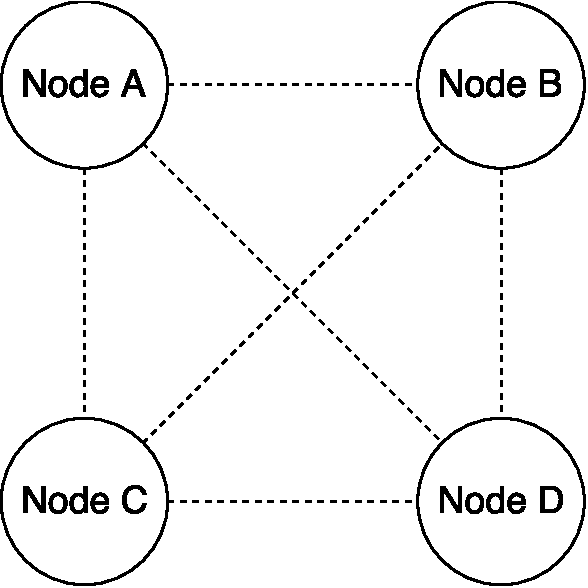
\includegraphics[scale=0.5]{images/computational_environment.pdf}
\caption{Computational environment, interconnected nodes} \label{fig:computational_environment}
\end{figure}

\subsection{Storage of data} \label{subsec:design_storage}
All information collected, such as how many replicas are currently executing, and on which nodes they are running, must be globally available and accessible from every node in the system. If stored on a single node, that information is lost in case that node fails. Also, if a remote database is used, a single-point-of-failure is introduced, resulting in a system where the reliability is no more than the reliability of the database. 

Instead, to achieve a redundant storage in our model, Distributed Hash Table (DHT) is used, which efficiently avoids having a single-point-of-failure. More specifically, the DHT implementation used is Kademlia, and we refer to~\cite{kademlia} for further info about DHT and Kademlia. The reason for choosing this approach is a result of Calvin, the framework in the model was implemented and evaluated, already using Kademlia. Calvin is further described in~\cref{subsec:design_calvin}.

When storing data using DHT, the data is first stored locally and later flushed, i.e. sent to other nodes. When a task is replicated to another node, the replication must only be considered successful if the storage is properly updated and the information shared to other nodes. Otherwise, the replication may only be partially reflected in the storage and use of this data will be useless. 
%TODO this text needs work

\subsection{Application model} \label{subsec:design_app_model}
The fault-tolerant framework presented in this paper is general and may be used in various contexts. However, it is particularly of value for long running applications and services running in dynamic environments, and where a certain level of reliability must be met. Long running applications are particularly vulnerable to failure because they usually require many resources and usually must produce precise results~\cite{relGridSystems}.

In this paper we use a simple example application in our experiments. The application can be modelled as shown in~\cref{fig:app_model}. The node $A$ shown in the figure could for example be a service for which we require a certain reliability. In contrast to ~\cite{algoOptTimeMaxRel, optTaskAllocationForMaxRel, taskAllocation, taskAllocationSwarm, algoMaxRelEndToEndConstraint, algoMinExTime, schedReplicas}, no assumptions are made about the execution time of the application. While our model is general, it's particularly beneficial for long running applications and services, as they in large-scale distributed environments are required to stay operational even in the case of unpredictable failures~\cite{imprRelAdaptRL}.

A typical example of a long running application is stream data processing, where a continuous stream of data is sent to a service which performs some computations on the data, and sends a result to a receiving process. The execution time is unknown, and in case of a failure, data may be lost. By sending the data to several replicas, redundancy is achieved and reliability thereby increased, as the probability of at least one replica produces a result increases.

\begin{figure}[!hbt]
\centering
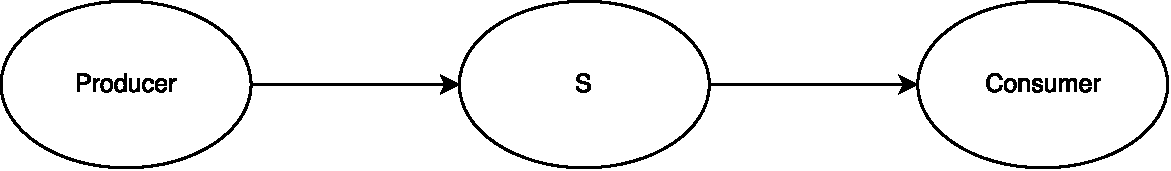
\includegraphics[scale=0.5]{images/app_model.pdf} 
\caption{An application model where a producer transmits data to a task $S$, which transforms the data, and sends the result to a consumer. $S$ may be seen as a task or service running in a cluster and requiring a certain level of reliability.}\label{fig:app_model}
\end{figure}

\iffalse
COMMENT: we should have some real examples of applications which would benefit from using our framework. ?
\begin{itemize}
\item telephone system?
\item video trans-coding when streaming video to mobile phone? In this case one could imagine a case where a video file is located on a server with limited processing power. The video could therefore be streamed to another server in the cluster, with more processing power, which encodes it on the fly and stream the result to the user. To keep a continuous stream of data to the user, even in the case of failure of the encoding server, one could replicate the task and stream the video to several servers which encode and transmit the results to the user. While this would increase the amount of transmitted data to the user's mobile, it would also increase the user experience.
\item Long running simulations? \cite{relModelDistSimSystem}
\end{itemize}
\fi

\iffalse

COPIED:
“Services in large-scale distributed environments (e.g., The Internet of Things [15]) are required to stay and continue operating even in the presence of malicious and unpredictable circumstances; that is, their processing capacity must not be significantly affected by the user requirements [11,8] “ \cite{imprRelAdaptRL}.
\\\\
COPIED: “Most workloads are large-scale long-running 3D scientific simulations, e.g. for nuclear stockpile stewardship. These applications perform long periods (often months) of CPU computation, interrupted every few hours by a few minutes of I/O for checkpointing. “ \cite{studyOfFailures}
\\\\
COPIED: “given the long execution times of many of the parallel applications that we are targeting – those in the scientific domain at national laboratories and supercomputing centers. “ \cite{implicationsOfFailures}. 
\\\\
COPIED: "The end result is that long-running, distributed applications are interrupted by hardware failures with increasing frequency" \cite{surveyFaultParallel}.

\fi

\subsection{Replication scheme} \label{subsec:design_repl_scheme}
As previously mentioned, reliability will be ensured by the use of replication. More specifically, active replication is used, where each replica receives the same input, and performs the same computations. \Cref{fig:app_model_replication} shows how the application in \cref{fig:app_model} looks after replicating task $S$ 4 times. It is also possible to have several services replicated, this scenario is shown in \cref{fig:extended_app_model}.

In contrast to the case with one \emph{primary} replica and several \emph{secondary} replicas, as described in \cref{subsec:background_replication}, we will adapt a fan-in fan-out model, where all replicas both receive the same input, but also all transmit its result to the consumer.

\begin{figure}[!hbt]
\centering
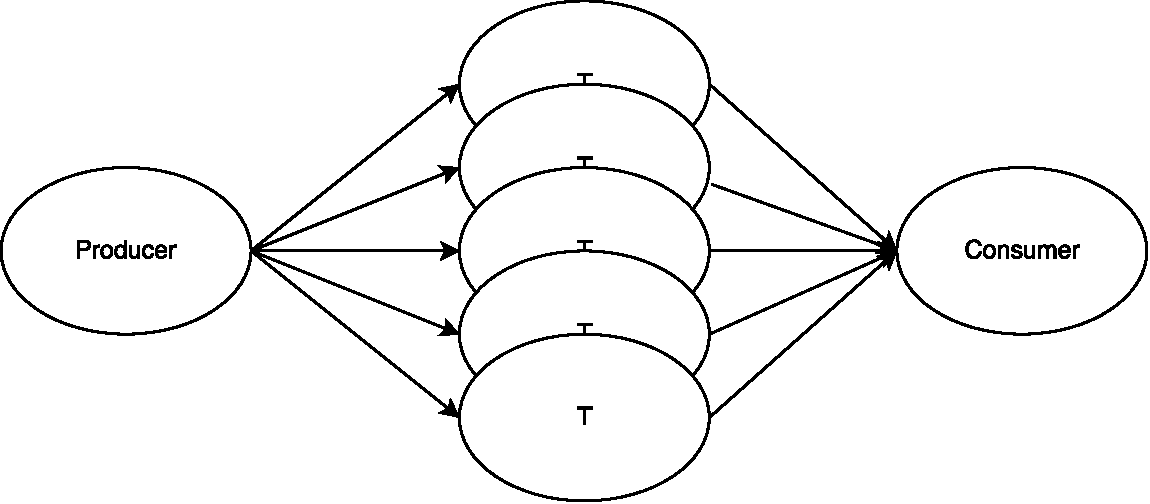
\includegraphics[scale=0.5]{images/app_model_replication.pdf} 
\caption{An application model where a task or service $S$ has been replicated 4 times.}\label{fig:app_model_replication}
\end{figure}

After replicating, the various replicas are likely to be un-synced. But, since assuming only deterministic calculations is done by the tasks replicated, given the same input they will all produce the same result, even if not synced. However, our model allows for easy extension to also include a majority decision at the consumer to determine whether or not the correct result was received. %TODO do we have to have this? I don't think it really affects our model right?

The process of replicating a task in Calvin, the framework in which our model was implemented, is further described in~\cref{subsec:calvin_replication}.

\subsection{Fault model} \label{subsec:design_fault_model}
In this paper, we adapt the \emph{fail-stop} fault model, which is described in~\cref{subsub:background_fail_stop} and commonly used when presenting fault-tolerance techniques~\cite{surveyFaultParallel}. Nodes in the system have one of two states: \emph{operational} or \emph{failed}. If a node fails, all running tasks on that node are dead. Furthermore, after a node has died, it will be restarted. However, the tasks that were being executed before it died will not be restarted when the node is restarted. The reason for why a node died is irrelevant. Our model do not care whether a link died, or it was a hardware failure, only that it stopped functioning.

Like~\cite{selfAdaptRel}, only system related failures are considered, assuming failures depends on the nodes, not the jobs running on them and the computations they perform. Furthermore, unlike the reliability models presented in~\cite{taskSchedulingReplication, taskAllocationSwarm, relAnalysisFRA}, the network is assumed fully reliable, and thus link failures are not accounted for. However, since evaluating our model in a real cluster, further described in~\cref{ch:evaluation}, link failures are in fact possible in our experiments, but in the case of a link failure a node will stop sending heartbeats, and will be assumed dead, further described in~\cref{subsec:heartbeats}.

\subsubsection{Failure distribution}
A commonly used assumption, also adapted in this paper, is that failures are statistically independent. Furthermore, failures are assumed to follow a Poisson process, as this seems to be widely accepted in the research community~\cite{experimentalFailureAssessment}. The Poisson distribution is defined as follows:

\begin{equation} \label{eq:Poisson}
P(k\ failures) = \dfrac{\lambda^k \cdot e^{-\lambda}}{k!}
\end{equation}

where $\lambda$ is the failure rate, i.e. the average number of failures occurring in time \emph{t}. In our case \emph{t} represents the time it take to detect a node failure and spawn a new replica. From \emph{t} and \emph{MTBF} we can calculate the failure rate $\lambda$ as $\lambda = t/MTBF$. \Cref{eq:Poisson} can therefore be re-written as

\begin{equation} \label{eq:Poisson_during_time_t}
P(k\ failures\ during\ time\ t) = \dfrac{\left(\dfrac{t}{MTBF}\right)^k \cdot e^{-\left(\dfrac{t}{MTBF}\right)}}{k!}
\end{equation}

The probability of surviving corresponds to having zero failures, and can be expressed as

\begin{equation} \label{eq:Poisson_no_failures}
P(0\ failures\ during\ time\ t) = \dfrac{\left(\dfrac{t}{MTBF}\right)^0 \cdot e^{-\left(\dfrac{t}{MTBF}\right)}}{0!} = e^{-\left(\dfrac{t}{MTBF}\right)}
\end{equation}

While most models using the Poisson process to model reliability assume constant failure rates, we assume they are constant only for a given period of time. By monitoring the system resources and registering failure times, allows for adapting the MTBF of a node. This is accomplished by using the time of the latest three failures to determine the MTBF as of~\cref{def:MTBF}. 

However, in order to use~\cref{eq:Poisson_no_failures}, the MTBF of a node must be available, and to calculate a node's MTBF at least two failures must have occurred since not all nodes are alive at time zero which is assumed by~\cref{def:mttf}. However, the system still need to be able to calculate the reliability for a node, even if the node has not yet failed. Therefore, a default value for the MTBF will be used in the experiments when no failure data is available for a node, or if it has not yet failed twice. In a real situation, the default value could be based on past failure data for resources of similar type. The default value used in the experiments is further described in~\cref{sec:eval_values}.

As time goes and nodes fail, the time of failure for nodes are stored, the system will get more precise values for the MTBF for the nodes in the system. By using the latest three failure times, one can adapt the MTBF as nodes start failing more or less often. The time it takes to detect node failure and spawn a new replica is further discussed in~\cref{sec:design_time_t}.


\section{Monitoring} \label{sec:design_monitoring}
Monitoring the system is crucial for achieving an entirely dynamic system, both in which the required reliability is met over time, but also not to use more resources than necessary. One must know both where replicas are executing and be able to detect node failures.

The sharing of resource information is done using a push strategy, as described in~\cref{sec:background_monitoring}. Information are periodically sent to all other nodes in the system in a multicast fashion, and a heartbeat system is used to detect node failures.

\subsection{Heartbeats} \label{subsec:heartbeats}
The ability to detect node failures is crucial for knowing when a new replica is needed in order to keep the required reliability. Furthermore, since the reliability model presented in~\cref{sec:design_reliability_model} is based on a \emph{mean-time-between-failures} for the nodes in the system, it is based on the assumption that node failures are detectable. 

To achieve this, a heartbeat system is used, where nodes periodically send UDP messages, called heartbeats, every $T_h$ seconds. The heartbeats contain a node identifier and are sent to all the other nodes in the system. Nodes are considered operational as long as heartbeats are received from them, and if no heartbeat is received from a node for $T_{timeout}$ seconds, the node is assumed dead.

In the experiments conducted, see \cref{ch:evaluation}, $T_h$ was set to 0.2 seconds, and $T_{timeout}$ to 0.5 seconds. These values should be modified in a real setting. For the experiments, a high-bandwidth low-latency cluster was used, why the frequency could be quite high and the timeout time relatively low. 

As further described in~\cref{sec:node_failure_detection_time}, these values also affect the reliability model, and thereby the number of replicas needed. A higher frequency and lower timeout means a shorter time in which the system is in a vulnerable state, and therefore a lower number of replicas may be needed to reach the required reliability. On the other hand, higher frequency means increased network traffic in the system as more heartbeats are being sent, although the size of a heartbeat message is quite low. %TODO mention message size?

\subsection{Monitoring system reliability} \label{subsec:monitoring_system_rel}
In order to ensure the optimal number of replicas is used over time as the properties of the system varies, the system and its running applications or services must be periodically monitored. 

In our model, the reliability of the running applications are monitored periodically. If the reliability is not met, appropriate actions are taken, which is further described in~\cref{sec:design_sched_alg}.

On the other hand, if the required reliability is met, more replicas than necessary may be used to reach that reliability level. One must therefore minimize the number of replicas by moving the replicas to more reliable nodes, and deleting replicas on less reliable nodes as long as the required reliability is still met. The algorithm for optimizing is further described in~\cref{subsec:design_optimization}.

In the experiments, applications were monitored and the optimization algorithm run every five seconds.

\section{Reliability model} \label{sec:design_reliability_model}
%TODO Maybe change section name
In this section the reliability model used in our experiments is presented. Note that the scheduling algorithm presented in~\cref{sec:design_sched_alg} is not dependent on the reliability model used.

\subsection{Definitions} \label{subsec:design_definitions}
In this paper, we use the following definitions of reliability:
\begin{definition} \label{def:single_task_reliability}
The reliability of a process is the probability that the resource on which the process is running is functioning during the time of execution.
\end{definition}

For multi-task applications, where the tasks use more than one resource, reliability is defined as
\begin{definition} \label{def:multi_task_reliability}
The reliability of a multi-task process is the probability that the tasks being executed for a given time without experiencing any type of failure (internal or external) during the time of execution.
\end{definition}

Finally, for long running applications or services, where a replication scheme is used, the reliability can be defined as \cite{effTaskReplMobGrid}
\begin{definition} \label{def:task_replica_reliability}
The reliability of a process, with $n$ task replicas, is the probability that at least one replica is always operational. This can be expressed as the probability that not all replicas fail during the time from that a task replica dies, until a new replica is operational.
\end{definition}

\subsection{Expressing reliability}\label{subsec:design_reliability}
Using replication and the reliability definition defined in~\cref{def:task_replica_reliability}, the reliability of a task $T$ with $n$ replicas, is the probability that at least one replica is successful during a time $t$, where $t$ is the time from that a replica fails, until a new replica is operational. This corresponds to at least one replica surviving time $t$, i.e. not all replicas fail, and can be expressed as 

\begin{equation} \label{eq:task_reliability}
R_{T}(t) = 1 - \prod\limits_{k=1}^n f_{k}(t)
\end{equation}

where $f_{k}(t)$ is the probability that replica $k$ fails during time $t$. 

Since assuming tasks themselves do not fail unless the resources they use fail, the reliability of a task is dependent on the reliability of the resources it uses, not the number of replicas. Since only considering node failures, the reliability of a task $T$ with $n$ replicas, where the replicas are placed on $m$ different nodes, can therefore be expressed as

\begin{equation} \label{eq:task_reliability_2}
R_{T}(t) = 1 - \prod\limits_{k=1}^m F_{k}(t)
\end{equation}

where $F_k$ is the probability that node $k$ fails during time $t$. Using \cref{eq:resource_reliability} for describing the reliability of a resource, \cref{eq:task_reliability_2} can be re-written as

\begin{equation} \label{eq:task_reliability_3}
R_{T}(t) = 1 - \prod\limits_{k=1}^m (1 - e^{\frac{t}{MTBF_k}})
\end{equation}

Where $MTBF_k$ is the \emph{mean-time-between-failure} for node $k$. Using this model, reliability is only increased through replication if the replicas are scheduled on separate nodes. \Cref{eq:task_reliability_3} is based on the assumption that failures of nodes are statistically independent, which is a commonly used assumption as described in~\cref{subsec:background_failure_distribution}.

Given a time $t$, a required reliability level $R_{req}$, and assuming the replicas are running on $m$ separate nodes, we get

\begin{equation} \label{eq:desired_rel}
R_T(t) = 1 - \prod\limits_{k=1}^m F_{k}(t) \geq R_{req}
\end{equation}

which must be fulfilled by the system. Assuming that failure rates differ among resources, fulfilling \cref{eq:desired_rel} is a scheduling problem, since the number of replicas needed is dependent on which resources the replicas are executed on.

The scheduling problem to fulfill a reliability $R_{req}$ refers to selecting $n$ nodes on which to place $n$ replicas such as the reliability level of the task, expressed in \cref{eq:task_reliability_3}, exceeds $R_{req}$.

\subsection{Expressing time t} \label{sec:design_time_t}
The time $t$ used in \cref{eq:task_reliability_3} is the time it takes from that a failure happened, until a new replica is operational, and consists of the time it takes to detect the failure, and the time it takes to create a new replica. $t$ can therefore be expressed as 

\begin{equation} \label{eq:rep_time}
	t = T_f + T_R
\end{equation}

where $T_f$ is the time to detect that a node has failed, and $T_R$ is the time it takes to create a new replica. A new replica is created by sending a replication request to a node currently holding a replica, including a third node on which the new replica is to be created. The replication request is further described in~\cref{sec:replication_time}.

\subsubsection{Node failure detection time} \label{sec:node_failure_detection_time}
As described in~\cref{subsec:heartbeats}, heartbeats are periodically sent to all nodes in the system every $T_h$ seconds, and if no heartbeat is received from a node for $T_{timeout}$ seconds, it is assumed dead. Note that $T_h$ must be lower than $T_{timeout}$.

The timeout time of $T_{timeout}$ is only an upper bound for how long it takes to detect a node failure. A node may fail just before sending a heartbeat, or directly after, which will affect the actual time the node has been dead before it is detected. This corresponds to the best and worst case scenario. 

If a node A dies precisely before sending heartbeat $H_k$ to B, the last received heartbeat from A was $H_{k - 1}$. $T_{timeout}$ seconds after $H_{k - 1}$ was received, node B will assume A has failed. Node A will then have been dead for $T_{timeout} - T_h$ seconds.

In the latter case, node A dies directly after sending a heartbeat $H_k$, and $T_{timeout}$ seconds later node B will assume node A has failed. Node A has in this case been dead for $T_{timeout}$ seconds when node B assumes it has failed.

Assuming that the probability of a node dying just before and directly after sending a heartbeat is the same, we get a theoretical average detection time of $T_{timeout} - \frac{T_h}{2}$ seconds. 

An example of the best and worst case scenario is shown in~\cref{appendix:figures}, where $T_h$ and $T_{timeout}$ are set to 0.2 and 0.5 seconds respectively, which are the values used in the experiments.

In~\cref{eq:rep_time}, $T_f$ is set to the upper bound of $T_{timeout}$. This is safe since using a higher value than the actual time it takes, results in the calculated reliability is lower than the actual reliability.


\subsubsection{Replication request time} \label{sec:replication_time}
The time $T_R$ in~\cref{eq:rep_time} is the time from that a replication request is sent, until a new replica is operational and response is received. It consists of the time it takes to send a replication request to a node, for that node to replicate its replica to a another node, and send a response.

To know which node to send the replication request to, one must first find out on which nodes current replicas are running. Thereafter, since the reliability is dependent on which nodes the replicas are running on, not solely on the number of replicas, one must also find a node which has no replica already and include this in the request. Then, a replication request is sent, a new replica is created, and a response is received. The time $T_R$ can be expressed as in~\cref{eq:replication_request_time}.

\begin{equation} \label{eq:replication_request_time}
T_R = T_{query\ storage} + T_{replicate\ msg} + T_{r} + T_{response}
\end{equation} 

Where $T_{query\ storage}$ is the time it takes to find out which nodes currently hold a replica, $T_{replicate\ msg}$ is the time to send a replicate message to another node, $T_{r}$ is the time to replicate the task to another node, and $T_{response}$ is the time to send a response to the requesting node. The process of sending a replication request is shown in~\cref{fig:replication_request}. The part of querying the storage is excluded from this image.

%TODO change remove the dead none from the image and rename D to C?
\begin{figure}[!hbt]
\centering
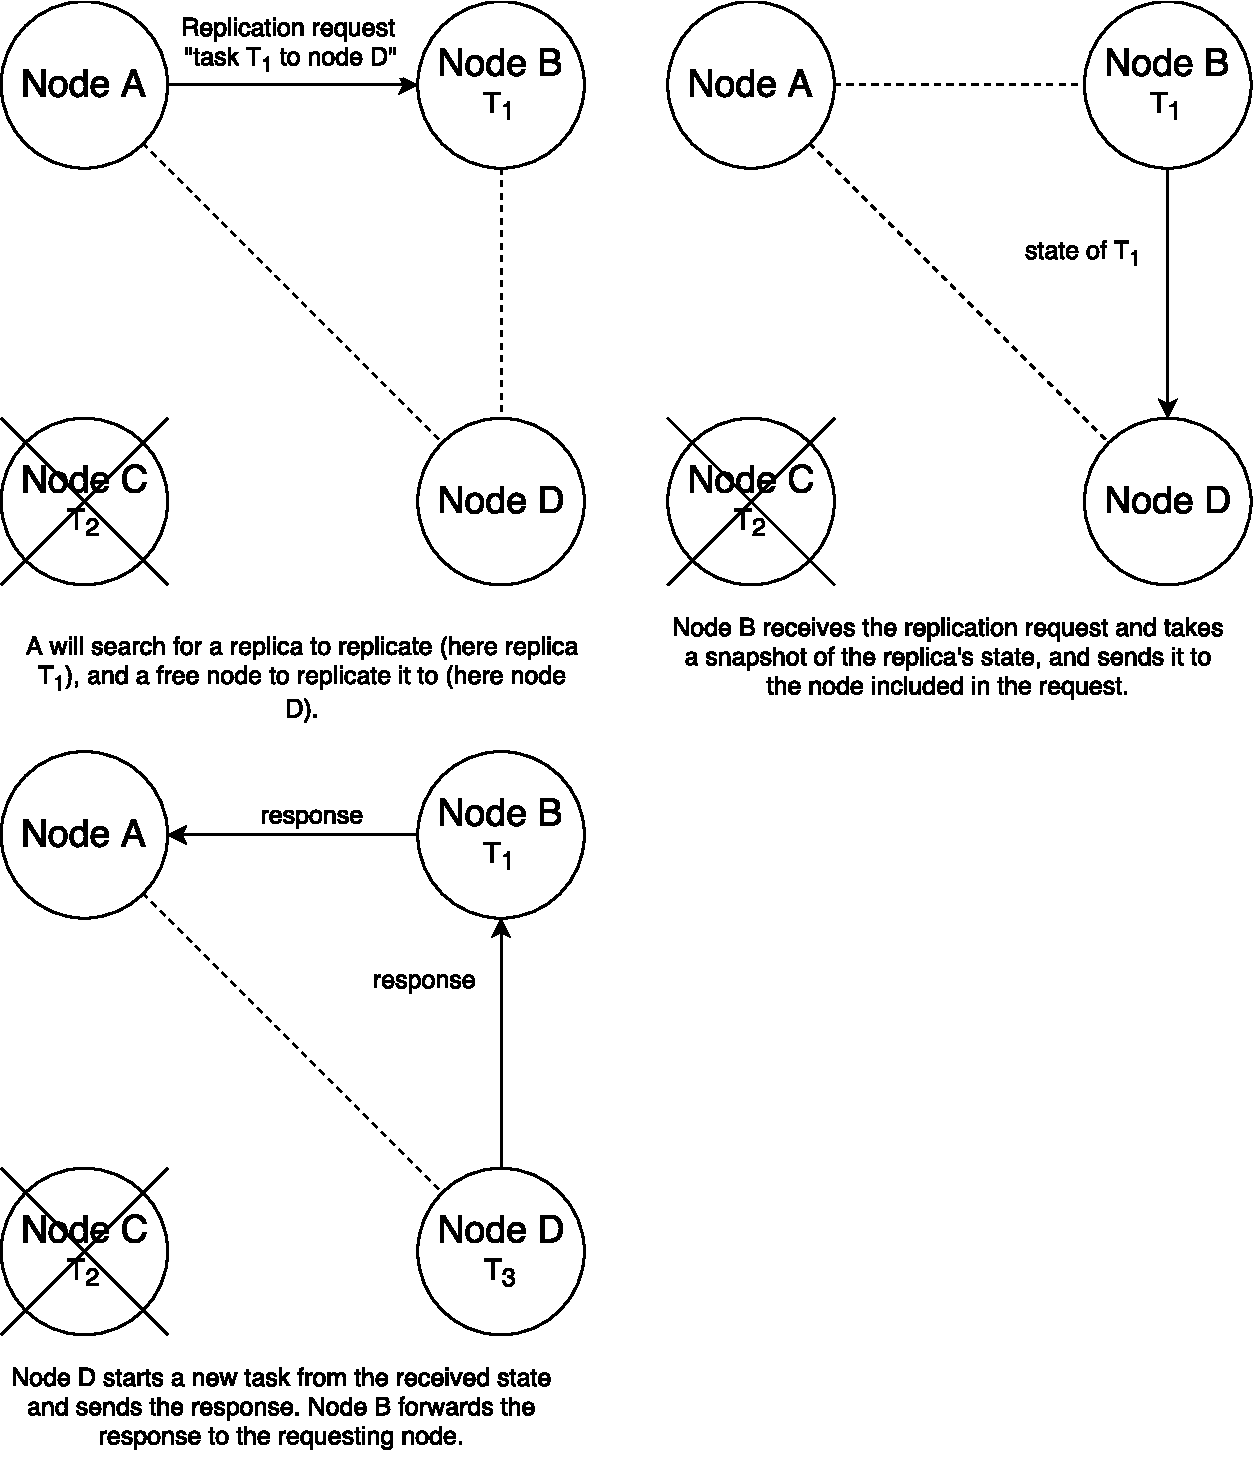
\includegraphics[scale=0.5]{images/replication_request.pdf}
\caption{The process of node A asking node B to replicate its replica a1 to node C, and receiving a response.}\label{fig:replication_request}
\end{figure}

As mentioned, the time $T_r$ is the time it takes to replicate a task. Depending on the state of the task to replicate, it is likely to be a significant part of the total time $T_R$. The time to replicate a task consists of the time to get the state of the task, serialize it, transmit it to the other node, de-serialize it, and create a new identical replica using that state, and send the response. 

\begin{equation} \label{eq:replication_time}
T_{r} = T_{get\ state} + T_{serialize\ state} + T_{transmit\ state} + T_{de-serialize\ state} + T_{setup\ new} + T_{response}
\end{equation} 

In our model, the time $T_{R}$ is measured and stored every time a replication takes place. Since $T_{r}$ depends on the size of the state, the time to replicate different tasks are likely to vary. Therefore, the time $T_{R}$ is stored per task type. Consequently, different types of tasks may require different number of replicas to reach the same reliability, as the reliability is dependent on the time $T_R$. \Cref{fig:replicas_depending_on_t} shows how the number of replicas needed to reach a reliability above 0.99, using nodes with a MTBF of 10 seconds, vary depending on the time \emph{t}.

\begin{figure}[!hbt]
\centering
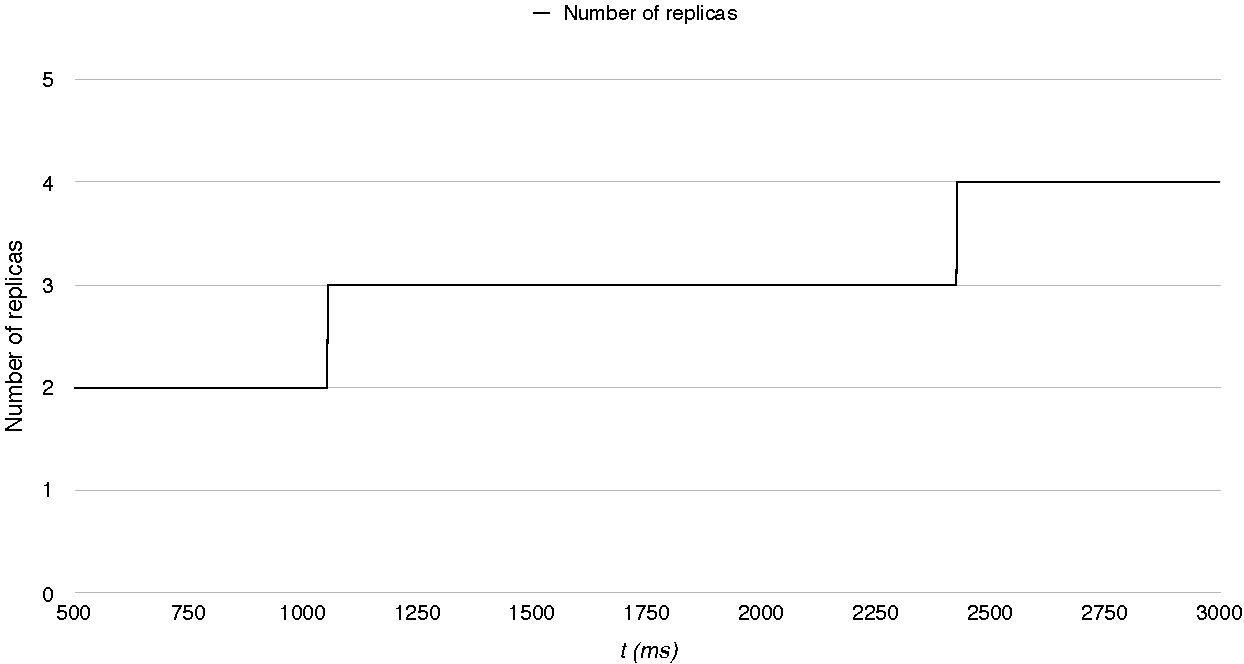
\includegraphics[scale=0.5]{images/replicas_depending_on_t.pdf}
\caption{The number of replicas needed to reach a reliabilty above 0.99, using nodes with a MTBF of 10 seconds, depending on the time \emph{t}.}\label{fig:replicas_depending_on_t}
\end{figure}


Other factors affect the time $T_R$. The node to which the replication request is sent may die before the replication is finished. The sender of the request assumed the receiving node has died if no response is received within a certain time. In this case, a new node is selected and asked to replicate its replica. When this happens, the time $T_R$, will be relatively high, as time was wasted sending the request to the first node. 

The situation can theoretically continue until there is no more nodes holding a replica. One could argue that this should be taken into account in the reliability model. Also the node being selected to run~\cref{alg:scheduling}, described below, may die, in case a new node is selected. These situations are further described in~\cref{sec:design_handling_failure}.

Instead of including the probability of these situations in the reliability model, a log-logistic distribution is first fitted to the previously registered times $T_R$. From the fitted distribution, the 95th percentile value is used as the value for $T_R$ in~\cref{eq:rep_time}. This means in 95 percent of the cases, the time $T_R$ will actually be lower than the value used in~\cref{eq:rep_time}. The reason for choosing log-logistic distribution is mentioned in~\cref{sec:eval_time_t}.

Finally, since assuming that all nodes are within the same cluster and that the latency between all nodes are low, we assume the time $T_R$ is independent on between which nodes the replication takes place. 

\section{Scheduling algorithm} \label{sec:design_sched_alg}
To fulfill~\cref{eq:desired_rel} using the minimum number of replicas, one could simply place a new replica on the most reliable node available, until the required level is reached. A greedy scheduling algorithm doing this, similar to one presented in~\cite{effTaskReplMobGrid}, and which fulfills~\cref{eq:desired_rel} is shown below:

%First we find which nodes that are available for placing a replica on. Secondly we filter the nodes with a load lower than a preferred level. If no preferred node is available we choose an unpreferred one.

\begin{algorithm}[H]
	\caption{Greedy scheduling algorithm to fulfill a given reliability} \label{alg:scheduling}
	\begin{algorithmic}[1]
	\Require{$R_{req}$ is the reliability to fulfill}
	\Statex
	\Procedure{Greedy scheduling algorithm}{}
	\State $current\ nodes\gets$ current nodes
	\State $operational\ nodes\gets $ operational nodes
	\State $available\ nodes\gets operational\ nodes \setminus \ current\ nodes$
	\State
	\Call{sort}{$available\ nodes$}
	\While {\Call{reliability}{$current\ nodes$} $\leq R_{req}$}
		\State $node\gets nodes.pop$\Comment{take the most reliable node}
		\State{$replica\gets new\ replica$}
		\State
		\Call{place replica on node}{$replica$, $node$}
		\State $current\ nodes\gets node$
	\EndWhile
	\EndProcedure
	\end{algorithmic}
\end{algorithm} 

\begin{function} 
	\caption{Sorts the given nodes in order of preference} \label{func:sort}
	Returns the given nodes in sorted order, with the most preferred nodes first. We only consider the nodes' reliability when sorting, but it can easily be changed to consider other parameters.
	\begin{algorithmic}[1]
	\Ensure{$nodes$ is the list to sort}
	\Statex
	\Function{sort}{$nodes$}
		\Statex\Comment{Add here to consider other parameters, such as nodes' loads, when sorting}
		\State
	    \Call{sort after reliability}{$nodes$}
	    \State \Return $nodes$
	\EndFunction
	\end{algorithmic}
\end{function}

\begin{function} 
	\caption{Calculates the reliability of the given nodes} \label{func:calc_reliability}
	\begin{algorithmic}[1]
	\Ensure{$current\ nodes$ is a list of nodes currently holding a replica}
	\Statex
	\Function{reliability}{$current\ nodes$}
		\State $n\gets current\ nodes.length$
		\State return $ \prod\limits_{k=1}^n R_{current\ nodes[k]}(t)$
	\EndFunction
	\end{algorithmic}
\end{function}

In our model, a new replica is placed on the most reliable node until the required reliability level is reached. However, we do not account for whether or not the selected node has enough available resources for the new replica, hence we do not consider system load. The scheduling algorithm is however independent of both the selection of nodes, and the calculation of the current reliability, why these two are two separate function calls. 

In our model, the reliability function uses~\cref{eq:task_reliability_2} for determining the reliability, and simply sorts available nodes after reliability, but they could both easily be replaced, e.g. by a more sophisticated reliability models, and to also consider nodes' loads when sorting them.

The algorithm is run at the time of deployment, but also every time a failure is detected, further described in~\cref{sec:design_handling_failure}.

\subsection{Optimization} \label{subsec:design_optimization}
\Cref{alg:scheduling} creates the minimal number of new replicas needed to reach the required reliability. However, it does not ensure the overall minimum number of replicas is used over time. As more reliable nodes become available, fewer replicas could be used while still meeting the required reliability. Therefore, \cref{alg:optimization} is periodically run, as part of the application monitoring as described in~\cref{subsec:monitoring_system_rel}.

\begin{algorithm} 
	\caption{Optimization algorithm} \label{alg:optimization}
	\begin{algorithmic}[1]
	\Procedure{Move to most reliable nodes}{}
	\State $current\ nodes\gets $ current nodes
	\State $operational\ nodes\gets $ operational nodes
	\State $available\ nodes\gets operational\ nodes \setminus \ current\ nodes$
	\State
	\Call{sort}{$available\ nodes$}
	\State
	\Call{sort}{$current\ nodes$}
	\State $least\_reliable\gets current\ nodes.pop$
	\State $most\_reliable\gets available\ nodes.pop$
	\While{$R_{most\_reliable}(t) > R_{least\_reliable}(t)$}
			\State $replica\gets $\Call{replica at}{$least\_reliable$}
			\State
			\Call{replicate to}{$replica$, $most\_reliable$}
			\State
			\Call{delete replica from node}{$replica$, $least\_reliable$}
			\State
			\State $current\ nodes\gets most\_reliable$
			\State $available\ nodes\gets least\_reliable$
			\State $least\_reliable\gets current\ nodes.pop$
			\State $most\_reliable\gets available\ nodes.pop$
	\EndWhile
	\EndProcedure
	\State
	
	\Procedure{Delete unnecessary replicas}{}
	\State $least\_reliable\gets current\ nodes.pop$
	\While {\Call{reliability}{$current\ nodes$}\ $\geq R_{req}$}
		\State $replica\gets $\Call{replica at}{$least\_reliable$}
		\State
		\Call{delete replica from node}{$replica$, $least\_reliable$}
		\State $least\_reliable\gets current\ nodes.pop$
	\EndWhile
	\EndProcedure
	\end{algorithmic}
\end{algorithm}

The first part of~\cref{alg:optimization} makes sure the most reliable nodes are used, by moving the replica on the least reliable node to the most reliable node available as long as more reliable nodes are available. To avoid putting the system in a vulnerable state, moving an actor consists of first creating a new replica, and later deleting the old one. By deleting first and then creating a new replica one risk not having enough replicas until the new replica is operational. Replicating first avoids this problem.

The second part make sure no unnecessary replica is used, by deleting the replica on the least reliable node as long as the required reliability is still met.

\Cref{alg:optimization} makes sure no unnecessary replicas are used. However, moving replicas to more reliable nodes may be unnecessary overhead if it does not affect the overall number of replicas needed. For example, moving from a node with a reliability of 0.999 to a node with reliability 0.9991 will perhaps not significantly increase the overall reliability, and if it does not result in another replica can be deleted, it may be unnecessary. \Cref{alg:optimization} does not account for this.

\section{Handling node failure} \label{sec:design_handling_failure}
In the case of a node failure, one must first determine whether or not any replicas were running on the failed node, and if so, determine whether or not new replicas are needed to still reach above the required reliability level. This is accomplished by running~\cref{alg:scheduling}. However, when a node fails, all other nodes in the system will detect its failure, since no node will receive heartbeats from it. If all other nodes start running~\cref{alg:scheduling}, one could end up in a situation where every remaining node creates a new replica. This will of course only increase the reliability, but we will no longer ensure the optimal number of replicas being used. 

To cope with this, selection process must take place to select a single node which will be responsible for deciding what actions to take. Since assuming a dynamic system where nodes fail and new nodes are introduced, this selection must be done every time a node dies. Furthermore, the selected node may also die before it managed to create any new replica. Therefore, all other nodes will send a \emph{lost node} request to the selected node. When finished, the selected node sends a reply back to all nodes it received a \emph{lost node} message from. If the sending nodes does not receive a reply for some time, they assume the selected node died, and a new selection process will begin.

The algorithm is shown below: % Om vi ska ha ":" får vi tvinga algoritmen att ligga här relativt till texten. Går att göra på något sätt, kommer inte ihåg just nu.

\begin{algorithm}\label{alg:node_failure}
	\caption{Handling a failed node}
	\begin{algorithmic}[1]
	\State $operational\ nodes\gets $ operational nodes
	\State
	\Call{sort after ID}{$operational\ nodes$}
	\Do
		\State $node\gets operational\ nodes.pop$
		\State
		\Call{lost node request}{$node$}
		\State {wait for reply}
		\State $reply\gets reply\ from\ node$
	\doWhile {$reply\ is\ not\ successful\ OR\ request\ timeout$}
	\end{algorithmic}
\end{algorithm}

A small example is presented in~\cref{fig:handling_node_failure}. In the situation shown in the figure, there are 4 connected nodes, A, B, C and D, and the node C has just failed. When the other nodes (A, B and D) detect the failure they will select the node with the highest ID, in this case node A, and inform it that node C has failed. Node A will then determine which actions to take.

\begin{figure}[!hbt]
\centering
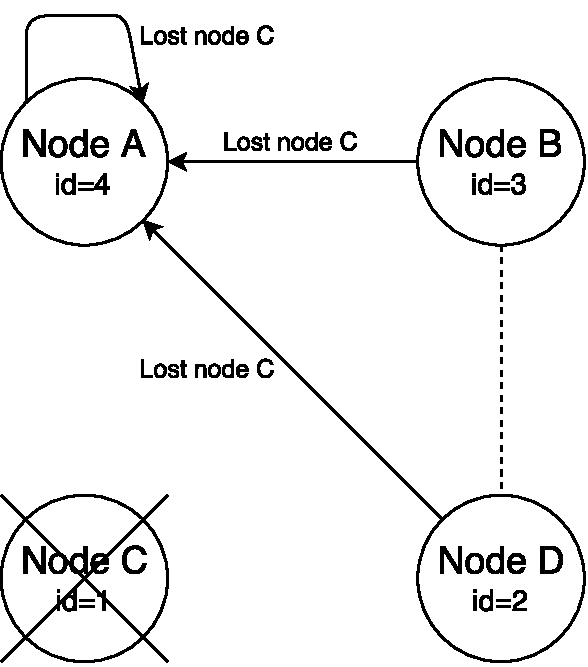
\includegraphics[scale=0.5]{images/handling_node_failure.pdf}
\caption{4 interconnected nodes after nodes A, B and D have detected the failure of node C.}\label{fig:handling_node_failure}
\end{figure}

\subsection{Selecting node}
As described, the node responsible for handling the detected failure is the node with highest ID among the nodes still being operational.

If the selected node determines a new replica is needed, it will send a replication request to a node currently holding a replica. If the selected node is one of the nodes holding a replica, there is no need for a replication request, since the node could simply replicate its own replica. One could therefore get rid of a replication request if one selected a node currently holding a replica in the selection process. However, to find out which nodes currently hold a replica, one must query the storage used, as described in~\cref{sec:replication_time}. Whether or not a centralized database is used, or DHT as used in Calvin where our model was implemented, this would result in every node detecting the failure querying the storage, and this approach is not scalable. Therefore, the selected node is any of the nodes still operational, and solely the selected node will query the storage for the information needed to handle the failure.

\section{Self-adapting} \label{sec:design_self_adapting}
Adaption refers to changing the behaviour depending on the changing state of the system. For a distributed system, resources most be continously monitored in order to adapt to changing behaviour~\cite{imprRelAdaptRL}.

To ensure a certain level of reliability, the framework must ensure that the current state of the system is taken into account when determining the number of replicas needed. Furthermore, the system and the running jobs must be continuously monitored, and the number of replicas must be increased if the reliability of a running job decreases below the desired level, or, the number of replicas must if possible be decreased in order not to waste resources.

When monitoring the system, all parameters used in the reliability model must be monitored. In our case, we consider only the nodes' mean-time-between-failures, the time to detect node failures and the time it takes to spawn a new replica. Therefore, all nodes' failure times, and the time to create new replicas are registered. The time to detect failure is as mentioned in~\cref{sec:node_failure_detection_time} static.


% TODO machine learning section?
\iffalse
TODO: If we have time: - we didn't :) Move this to discussion?
Furthermore, we will take node CPU usage, and the time of day of the event into account in our fault model. This is based on that resource failure depends on both system load and time of day~\cite{implicationsOfFailures, studyOfFailures}.
\fi

\iffalse
COPIED: “adaptation to changing conditions is achieved by both adaptive scheduling and adaptive execution” \cite{evalOfGridRel}.

COPIED:
"the distributed systems require consistent and iterative monitoring for valuation resources’ behaviors and processing requirements. Therefore, an autonomous, scalable and highly dynamic learning approach is deserved \cite{imprRelAdaptRL}

%TODO predict future MTBF? machine learning? cpu, memory usage, network load, etc.

COPIED:
“The individual component can be monitored in real time and updates the parameters dynamically for the exponential distribution. The monitored information is simple: just the number of failures over the total running time of this component which has actually been recorded by log files in today’s grids. Such a dynamic updating scheme can further validate the exponential assumption, though we may relax the above assumption somewhat to allow reasonable or gradual change in the failure rate (such as wear out) because, during a short enough period of service time, the parameter cannot change too much and using the latest value should be a good approximation “ \cite{hierarchicalRelModeling}.

COPIED: “in the proposed system, we need to determine the degree of over-provisioning or job replicas as small as possible in order to minimize the system overhead “ \cite{designFaultTolerantSched}.
\fi

\section{Implementation} \label{sec:design_implementation}
For implementing our model, we use an actor based application environment called \emph{Calvin}. Below follows a brief description of the main parts of the Calvin framework, for further info we refer to~\cite{calvin}.

\subsection{Calvin} \label{subsec:design_calvin}
Calvin is an actor-based application environment for leight-weight IoT applications, and is written in Python. It was developed by \emph{Ericsson} and made open source in the summer of 2015. While Calvin is an application environment for IoT applications, is suites well for implementation of our model.

\subsubsection{Storage} \label{sec:calvin_storage}
Calvin uses the Kademlia implementation of a DHT. This enables that any data stored by a node is distributed and available for all nodes in the network. DHT will not be further explained in this thesis, instead we refer to~\cite{kademlia} for further information about DHT and Kademlia especially.
%TODO Mention that there is an alternative way of storing, e.g. the proxy storage

\subsubsection{Actor model}
An application in Calvin consist of a set of connected \emph{actors}. An actor usually represents part of a device, service or computation. Actors communicate by sending data, called tokens, on their out-ports to other actors in-ports. 

Multiple actors may send data to another actors in-port, and an actor's out-port may have several receivers. For each receiver of outgoing messages, or sender of incoming messages, there is a separate queue of tokens to process.

The runtime, see~\cref{sec:calvin_runtime}, in which an actor is executing is responsible for the communication between runtimes and between actors.

The state of an actor is needed when replicating an actor. In Calvin, the state of an actor consists mainly of actor type, in-port and out-port connections, and for each port a queue with data to process or to send, and read and write positions for the incoming and outgoing queues. The queues is the major part of the message size.

The actor model corresponds well to the kind of applications and tasks described in~\cref{subsec:design_app_model}, as they perform deterministic calculations.

\subsubsection{Runtimes} \label{sec:calvin_runtime}
The Calvin framework use a concept of \emph{runtimes}. A mesh of connected runtimes makes up the distributed execution environment on which one can deploy application. A runtime is a self-managed container for application actors and provides data transport between actors both within the same runtime and between different runtimes.

Each runtime has a \emph(storage), all the information stored in storage is first stored locally and later flushed, i.e. distributed in a multicast approach.

\subsubsection{Replication} \label{subsec:calvin_replication}
The process of replicating an actor in Calvin starts with getting the state of the actor to replicate, serialize it, send it to the runtime in which the new replica is to be created. The receiving runtime must de-serialize the state and use it to create the replica and setup its port connections.

Part of creating the new replica is decoding the in- and out-ports' queues, which are part of the state. This processing is CPU bound and affects the total replication time, as shown in the experiment in~\cref{sec:eval_repl_time}.

\subsection{Our contributions to Calvin} \label{subsec:design_contributions} % ish?
Here follows a small description of the most important parts of our changes and new features in Calvin.

\subsubsection{Fan-in connectivity}
We extended the Calvin framework to allow a fan-out/fan-in connectivity model where actors can have multiple producers (fan-in) and multiple consumers (fan-out). Previously, only multiple receivers were allowed, but with our changes an actor's in-port could have multiple senders.

\subsubsection{Actor replication}
Previously, the framework allowed for dynamically migrating an actor from one runtime to another. We extended this functionality by allowing dynamic replication of actors. 

%Maybe mention that due to no consensus actors only use the first received value

\subsubsection{Node Resource Reporter}
To share various kinds of resources between runtimes, e.g. CPU usage as used in~\cref{sec:eval_replaceable_model}, we created a resource reporter actor. When a runtime is created, it automatically creates a resource reporting actor. The actor periodically reports the node's CPU usage to all connected runtimes. Furthermore, each node has a resource manager which stores the other nodes' usages.

%TODO we currently do not use the CPU usage, this is therefore not neccessary?

\subsubsection{Resource Manager}
Besides storing the connected nodes usages the resource manager stores information about node failures. If a node fails a time stamp and the failed node's usage is stored, among with the time it took to replicate a new replica for each of the actors which were running on the failed node.


\subsubsection{Heartbeat Actor}
The heartbeat system described in~\cref{subsec:heartbeats}, was implemented using actors. Each runtime creates a heartbeat actor when its started. The heartbeat actor listens for heartbeats as well as periodically sends heartbeats to other runtimes.

Unlike the resource manager, messages are sent using UDP instead of TCP. With TCP, an initial handshake it used to setup the communication channel. For a heartbeat system, this is unnecessary overhead. 

For every heartbeat sent, a timeout of 500 ms it set. When it timeouts, the runtime to which the heartbeat was sent is assumed dead, and when a heartbeat is received, all timeouts related to that runtime is canceled. When a timeout happens, \cref{alg:node_failure} and new replicas are created if needed to reach the required reliability.

\subsubsection{Application monitor}
Each runtime also periodically monitors the applications deployed to it, to ensure the required reliability is achieved by running \cref{alg:scheduling} and creating new replicas if needed. Also the optimization algorithm, is run as part of this monitoring.

\chapter{Evaluation} \label{ch:evaluation}
In order to validate our model, we conducted a set of experiments. The goal of the experiments were to show the three main properties of our model. First, that it dynamically ensures the desired level of reliability is met, despite the event of node failures, by dynamically creating new replicas when old ones are lost. Second, that it uses the optimal number of replicas by choosing the most reliable nodes, and also removing unnecessary ones. Finally, that it adapts to changing properties of the system.

\section{Values used in the experiments} \label{sec:eval_values}
As described previously, heartbeats were sent every 200 ms in all experiments, and nodes were considered dead if no heartbeat was received for 500 ms. The optimization algorithm was run every 5 seconds.

Furthermore, the reliability model is based on a node's MTBF and the time $T_R$. In order to determine the MTBF for a node, at least two failure times must have been registered. Before a node has failed twice, a default value is used. In all experiments, the default MTBF was 10 seconds.

In addition to the MTBF, a default value for $T_R$ must be used before any such times have been registered. The default value used in the tests was 2 seconds.

The state size of the actor replicated in the experiments was XXX MB.

\section{Computational environment} \label{sec:eval_comp_env}
In the experiments, a cluster consisting of 6 inter-connected servers with homogeneous hardware components were used. A laptop was also used when measuring the replication time. The specification of the servers and the laptop are described in~\cref{sec:server_spec} and \cref{sec:laptop_spec}. The various servers will be referred to as \emph{Gru}, \emph{Dave}, \emph{Kevin}, \emph{Mark}, \emph{Jerry} and \emph{Tim}.

As mentioned in \cref{ch:design}, the model was implemented in the IoT application environment Calvin. On five of the six servers used, one or two (depending on experiment) Calvin runtimes were started. The runtimes were used to represent actual nodes, and were periodically killed and restarted to simulate node failure. On the sixth server a single runtime was started, which was not killed. The reason for having a stable runtime in the experiments is described in~\cref{sec:eval_application}. In the experiments, the runtimes are referred to as nodes.

\subsection{Simulating node failure} \label{sec:simulating_node_failure}
As mentioned, the servers used in the experiments had homogeneous hardware components, but varying failure rates were simulated by killing and restarting the runtimes with varying rates.

The process of killing and restarting is shown in~\cref{alg:simulating_node_failures}. If a node was to have a MTBF of 15 seconds, the time between failures followed a normal distribution with mean 15 and standard deviation of 1. Since the tests only ran for a couple of minutes, the actual MTBF for a given node may during the duration of a test be either lower or higher than the given MTBF. The reason for using values from a normal distribution with mean equal to the given MTBF, instead of simply the given MTBF, was to simulate a more realistic situation. If all runtimes were given the same MTBF and slept exactly that time, they would all have died at the same time, given that they were started at the same time. Furthermore, if we would have waited some time before starting each runtime, two runtimes would perhaps never die at the same time. By picking values from a normal distribution, two or more runtimes may fail at the same time during the time of the experiments.

\begin{algorithm} 
	\caption{Simulating node failures} \label{alg:simulating_node_failures}
	\begin{algorithmic}[1]
	\While {$true$}
		\State
		\Call{start runtime}{}
		\State $t_{s}\gets \mathcal{N} (MTBF,1)$
		\State
		\Call{sleep $t_{s}$}{}
		\State
		\Call{kill runtime}{}
	\EndWhile
	\end{algorithmic}
\end{algorithm}

\subsection{Node specification}
\subsubsection{Server specification} \label{sec:server_spec}
The servers used in the experiments all had a Intel(R) Xeon(R) CPU E5-2420 v2 of 2.20 GHz and 24 GB RAM. Furthermore, they were all connected with a 1000 Mb/s link with a latency of less than 0.2 ms. The OS installed on the servers was Ubuntu 14.04 LTS.

\subsubsection{Laptop specification} \label{sec:laptop_spec}
The laptop used in the experiment where the replication time was measured, was a Dell Vostro v131 with a Intel i5, 2.3 GHz processor, 4 GB 1333 MHz RAM. It was equipped with a SSD with a read speed of 540 MB/s and a write speed of 520 MB/s. Furthermore the installed OS was the same as for the servers, Ubuntu 14.04 LTS.

\section{Application used in experiments} \label{sec:eval_application}
The Calvin application used in the experiments was of simplest form, consisting only of a producing actor, a service actor and a consuming actor. The producing actor produced integer numbers and sent those to the service actor which simply forwarded them to the consuming actor, which printed the values to standard out. 

A predefined level of reliability was required only for the service actor, and it was therefore the only one being replicated. As neither the producing nor the consuming actor were replicated, the whole application would have died in case the runtime on which they were deployed died. Therefore, they were both placed on a stable runtime, which was not killed. The service actor however, was only deployed to the unstable runtimes.

The computational environment and the application is shown in~\cref{fig:evaluation_application}.

\begin{figure}[!hbt]
\centering
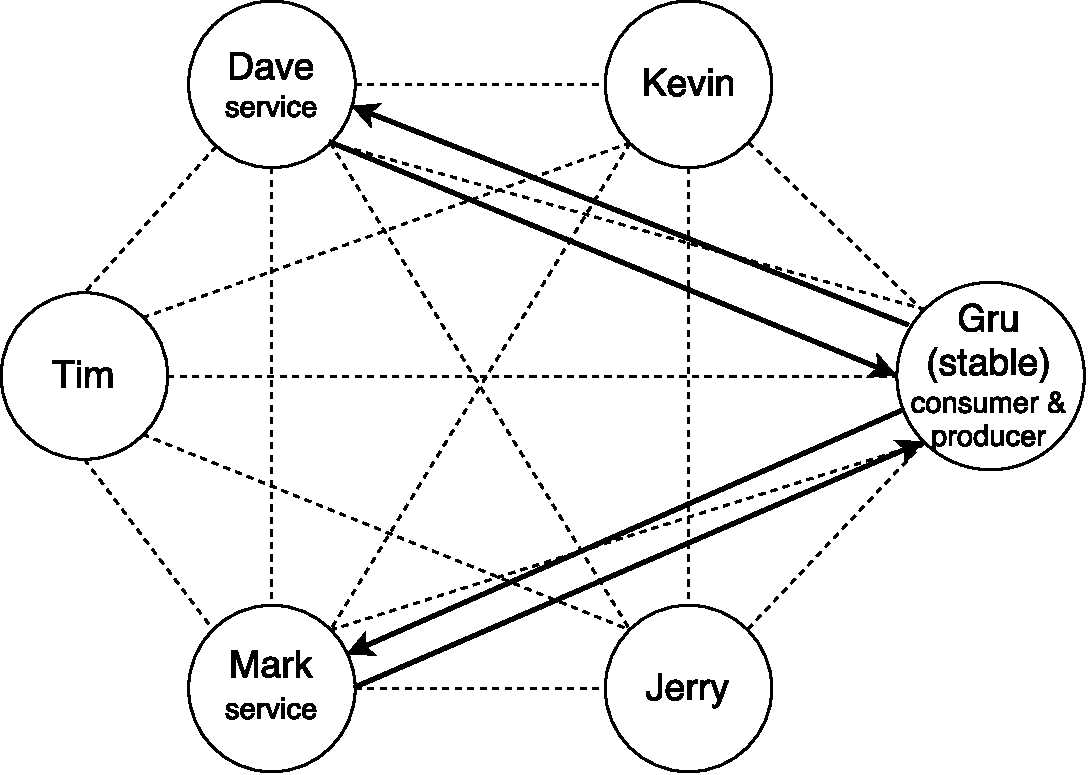
\includegraphics[scale=0.5]{images/evaluation_application.pdf} 
\caption{The computational environment used in the experiments. In this example, there is a producer and consumer on Gru, and two replicas of the service located on Dave and Mark.} \label{fig:evaluation_application}
\end{figure}

\section{Experiments}

\subsection{Measurement of time $T_R$} \label{sec:eval_time_t}
As mentioned in~\cref{sec:design_time_t}, the time $t$ is the time it takes from that a node on which a replica is running dies, until a new replica is operational, and depends on the time it takes to detect that the node died, and the time it takes to create a new replica. 

The time for detecting that a node has died, $T_f$, in~\cref{eq:rep_time} is static and set to the upper bound of 500 ms as described in~\cref{sec:node_failure_detection_time}. While $T_f$ is static, the time for the replication request, $T_R$, varies. In order to find the best distribution for the times $T_R$, an experiment was conducted where the times were registered and later used to find a best fitting distribution.

Two Calvin runtimes were started on each of the non-stable servers, each with a MTBF of 10 seconds, and the required reliability was set to 0.99999.

\subsubsection*{Results}
The experiment ran for XXX minutes, and YYY times were registered.

The distributions tested were \emph{beta}, \emph{birnbaumsaunders}, \emph{exponential}, \emph{extreme value}, \emph{gamma generalized pareto}, \emph{inversegaussian}, \emph{logistic}, \emph{logalogistic}, \emph{lognormal}, \emph{nakagami}, \emph{normal}, \emph{rayleigh}, \emph{rician}, \emph{tlocationscale}, \emph{weibull}.

Matlab was used to determine which distribution best fitted the data, and the Bayesian information criterion was used to determine how good of a fit a distribution was.

\Cref{fig:distribution_results} shows the four best fitted distributions, with log-logistic being the best.


\begin{figure}[!hbt]
\centering
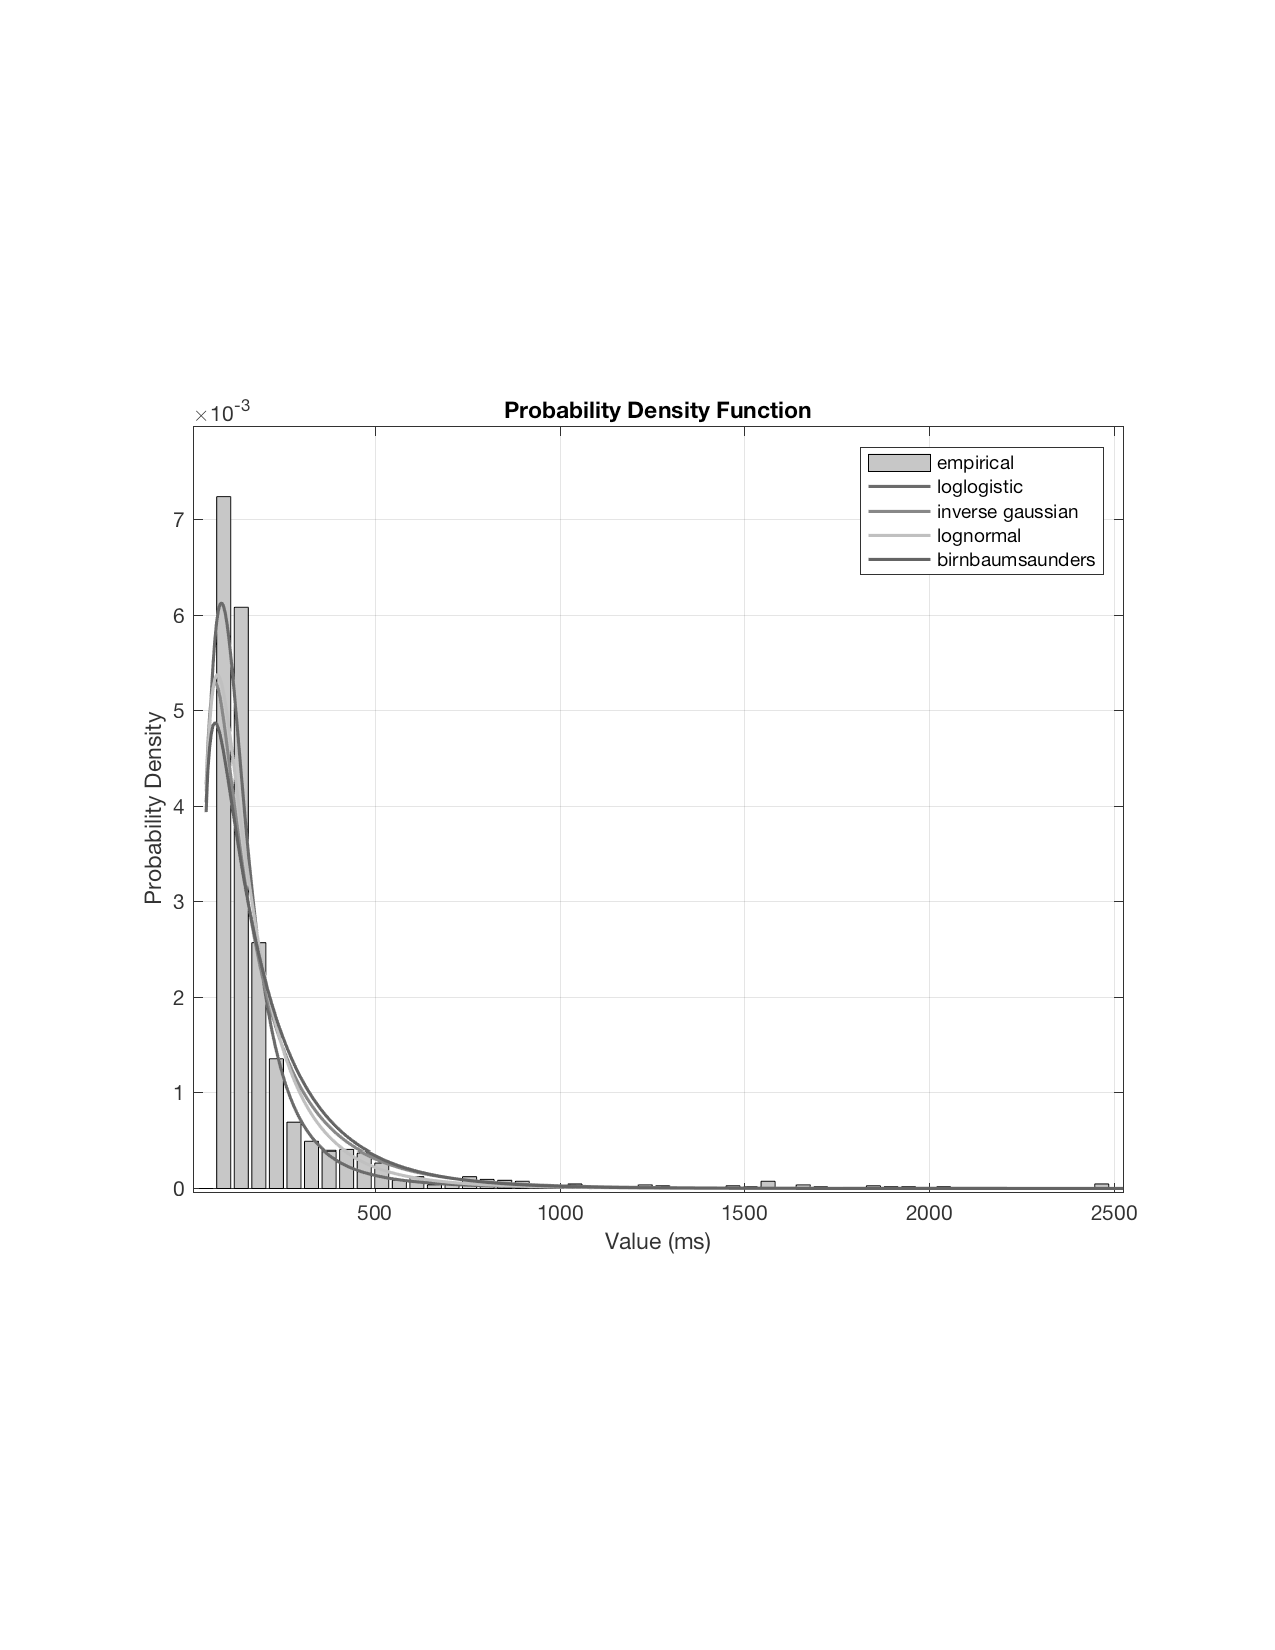
\includegraphics[scale=0.5]{images/results/distribution_results.pdf} 
\caption{Result for test~\ref{sec:eval_time_t}. The four best fitted distributions for the failure time data.}\label{fig:distribution_results}
\end{figure} 

\subsection{Measurement of node failure detection time} \label{subsec:eval_node_fail_time}
% Is this needed really?
As described in~\cref{sec:design_monitoring}, heartbeats are used to decide whether or not another node is healthy. If no heartbeat is received from a node within 500 ms, it is assumed dead. 

In order to measure the time it takes to detect a failed node, an experiment was conducted in which two servers were used, each with a Calvin runtime. One of the runtimes was periodically killed and restarted. Before killing the runtime, the current time was logged, and on the other node, the time was logged when the node was assumed dead, which was 500 ms after the last received heartbeat as described in~\cref{subsec:heartbeats}. The failing node was killed and restarted 50 times.

\subsubsection*{Results}
The average of the 50 measured times was 483.8 ms. This above the theoretical average of 400 ms, but lower than the upper bound of 500 ms. 
%TODO Calculate a confidence interval
% klockorna måsta vara synkade..

\subsection{Measurement of replication time} \label{sec:eval_repl_time}
The time it takes to replicate a task, depends on the size of the task state, which have to be sent to the new node. Using Calvin, the state of a task corresponds to the state of the actor representing the task. In Calvin, the state consists mainly of the queues of incoming and outgoing data for the actor's in- and out-ports, and any local variables the actor has.

In the following experiments, two runtimes were used, either on the same laptop or on two different servers. The application was first deployed to one of these runtimes, and the service actor was replicated to the other runtimes and the time measured. This was repeated for various sizes of the actor's state. The actor had only one out-port and no in-port, and in the first experiment the state of the actor was incrementally increased by increasing the size of a local variable, while in the second experiment it was increased by increasing the size of its output queue. The state of the actor is only one part of the total replication message. The other part is static, and its size during the experiment was 349 bytes.

The times measured was the time to serialize the state, send the state to the other runtime, de-serialize it, create and start the new actor, and send the reply.

Both experiments was conducted in two settings. In one, two servers were used with a runtime on each of them, while in the other, a laptop was used on which both the two runtimes were started. The specification of the servers and the laptop are found in~\cref{sec:server_spec} and~\cref{sec:laptop_spec}. For each state size, the actor was replicated 10 times and the times measured.

For three state sizes, 1, 50 and 100 MB, we measured the replication time 100 times and calculated the standard deviation of these values.

The goal of the experiment was to see how the replication time vary depending on the state size, in which part of the replication process most time is spent, and finally how the replication times varied.

\subsubsection*{Results - total replication time}
\Cref{fig:replication_time_server} and \cref{fig:replication_time_laptop} show how the total replication time vary depending on the state size when replicating from server to server and from laptop to laptop respectively. As shown, the replication time was higher when the increasing the queue size than  when increasing the variable size. This is due to the extra time needed when creating the new actor, when the values in queue are decoded. %TODO express the last sentence better...

As seen in the figures, the replication time is exponential. When replicating using the laptop, there is a big increase in time when increasing the state size from 200 MB to 400 MB. This is due to running out of memory, and the process started using the system's SWAP memory, which significantly reduced the performance. The increase in time is very big when increasing the queue size but not when increasing the variable size. This is probably due to the memory needed when decoding the queue when creating the new actor.

\begin{figure}[hbt!]
\centering
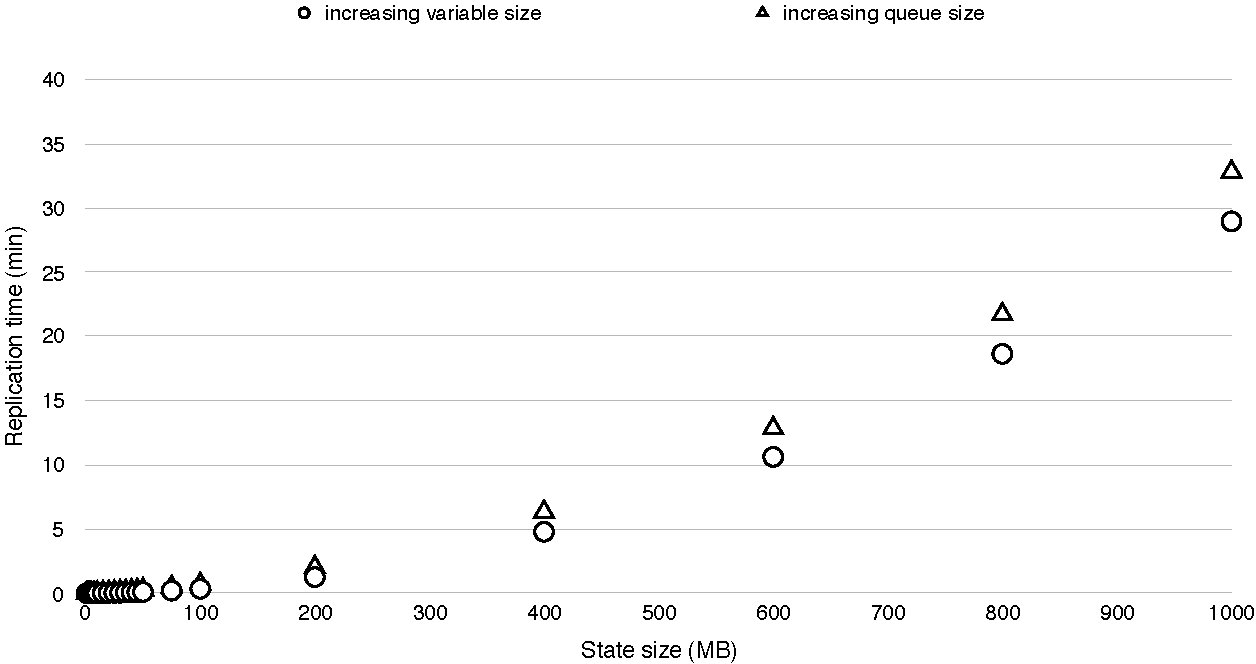
\includegraphics[scale=0.5]{images/results/replication_time/server.pdf} 
\caption{Result for test~\ref{sec:eval_repl_time}. The average replication time as a function of state size, where the state size was increased by increasing the size of one of the actor's variables.} \label{fig:replication_time_server}
\end{figure}

\begin{figure}[hbt!]
\centering
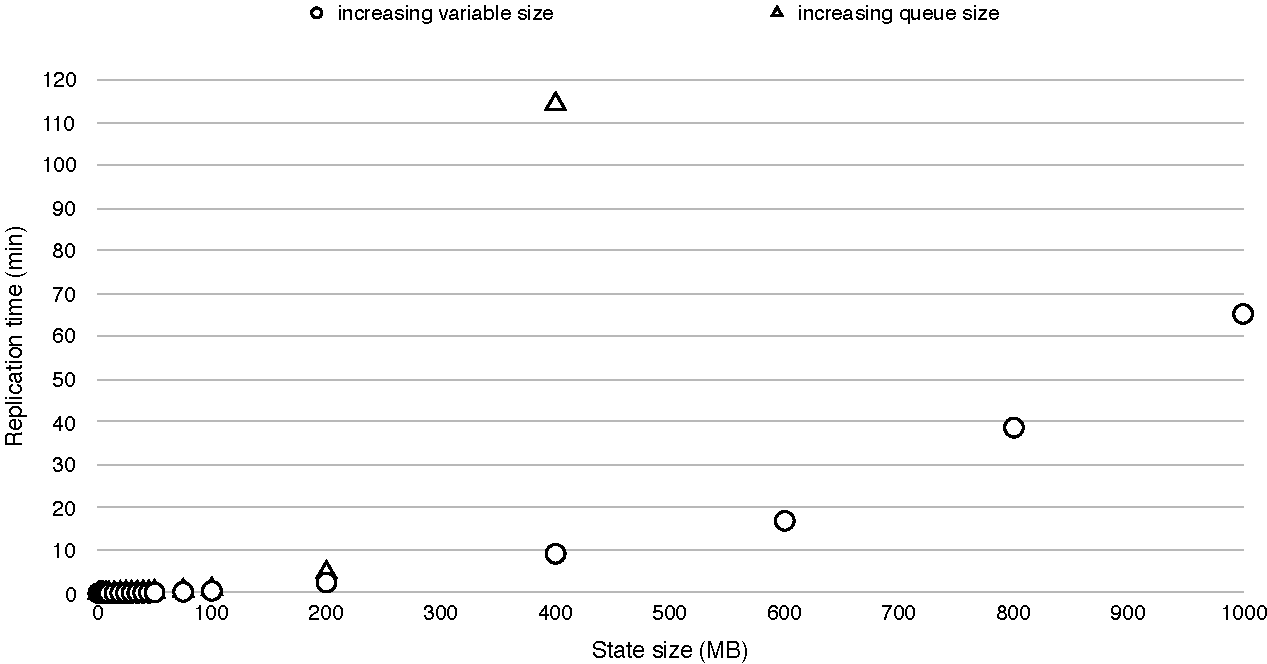
\includegraphics[scale=0.5]{images/results/replication_time/laptop.pdf} 
\caption{Result for test~\ref{sec:eval_repl_time}. The average replication time as a function of state size, where the state size was increased by increasing the size of the actor's port queue.} \label{fig:replication_time_laptop}
\end{figure}

\subsubsection*{Results - replication time parts}
\Cref{fig:replication_time_parts_server_variable}, \cref{fig:replication_time_parts_server_queue} show how much of the total replication time is spent on the various parts of the replication process when increasing the variable size and queue size respectively, and when replicating between the two servers. As shown, the time to create the new replica takes significantly larger part of the total time when increasing the queue size rather than the variable size. This is due to the time spent on decoding the queue's values as described above.

Furthermore, significantly more time is spent on transmitting the state to the other node for large state sizes. Hence for large state sizes, the replication time depends on the bandwidth of the links connecting the various nodes. For smaller state sizes, the replication time is more CPU bound.

%TODO needs work.
\Cref{fig:replication_time_parts_laptop_variable}, \cref{fig:replication_time_parts_laptop_queue} show how much of the total replication time is spent on the various parts of the replication process, when increasing the variable size and queue size respectively, and when the replication is done between two runtimes on the same laptop. Again, more time is spent on creating the new actor when increasing the queue size than when increasing the variable size.

 Furthermore, the time spent on transmitting the state increases when increasing the state size. However, when the state size is above 100 MB (when increasing the queue size), more time is spent on creating the actor, which is due to running out of memory as described before. In the experiment, this happened when the size was 200 MB or more. When this happens, the process needs to use the system's swap memory when creating the new actor. A 1333 MHz ram memory has a speed of approximately 21 GB/s, which compared to the SSD speed of 540 MB/s explains the significantly drop in performance.

\begin{figure}[hbt!]
\centering
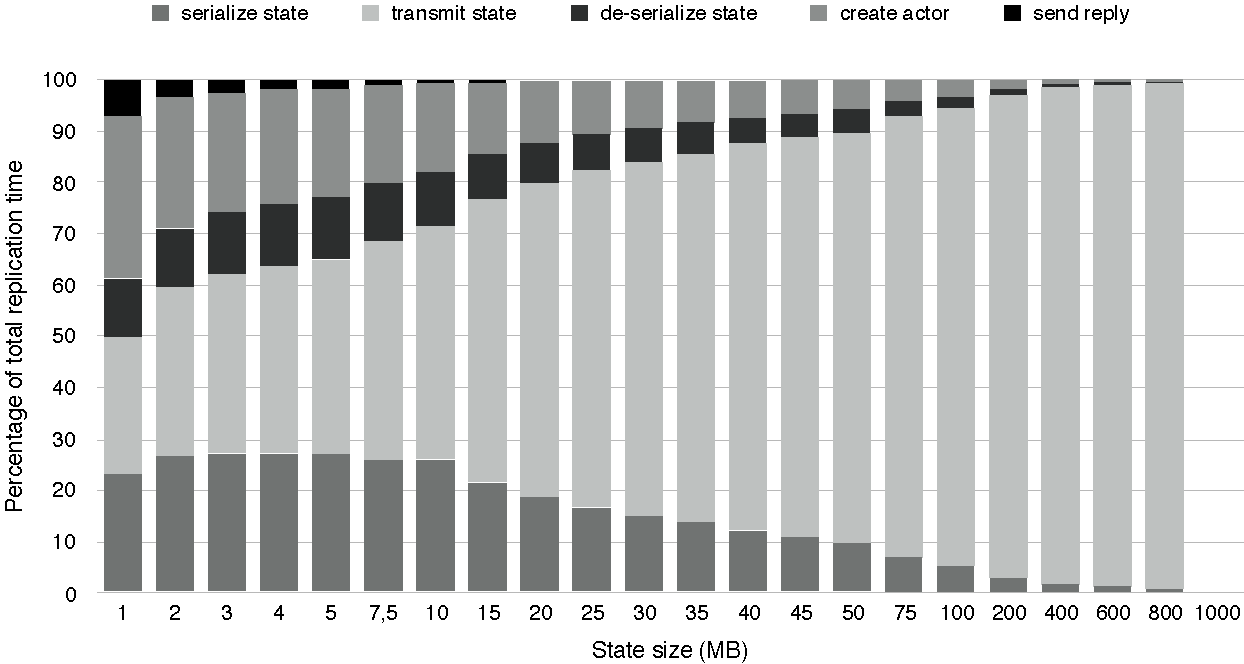
\includegraphics[scale=0.5]{images/results/replication_time/server_parts_variable.pdf} 
\caption{Result for test~\ref{sec:eval_repl_time}. Server to server, increased variable size} \label{fig:replication_time_parts_server_variable}
\end{figure}

\begin{figure}[hbt!]
\centering
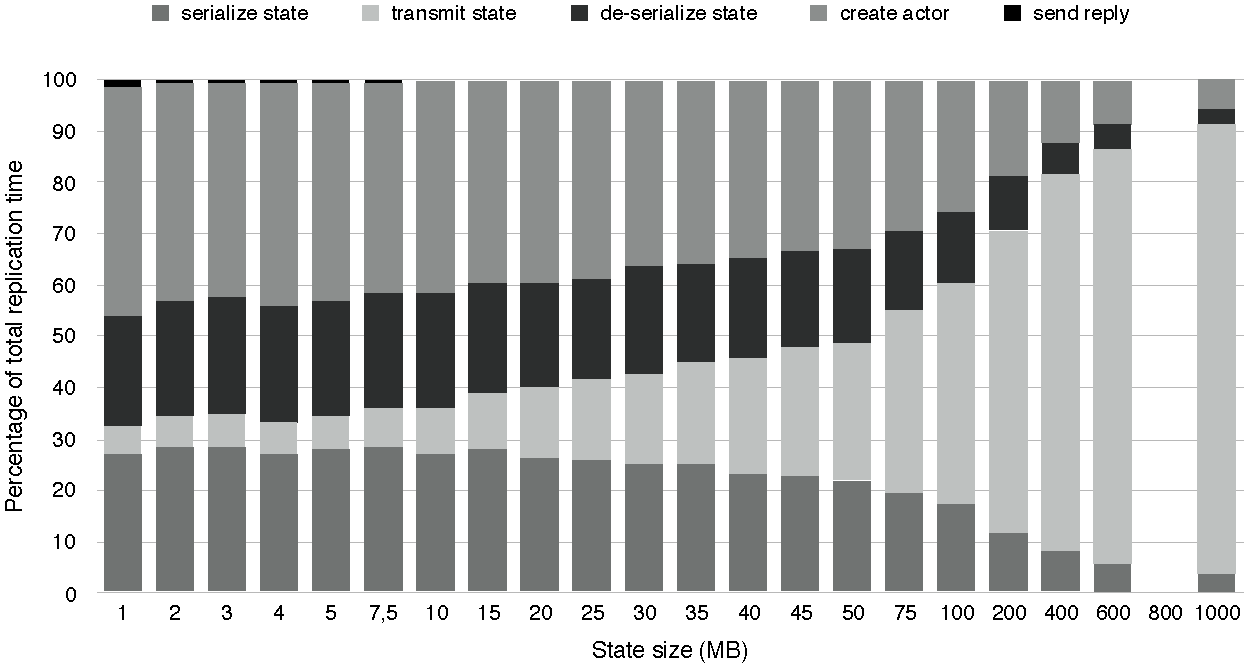
\includegraphics[scale=0.5]{images/results/replication_time/server_parts_queue.pdf} 
\caption{Result for test~\ref{sec:eval_repl_time}. Server to server, increased queue size.} \label{fig:replication_time_parts_server_queue}
\end{figure}

\begin{figure}[hbt!]
\centering
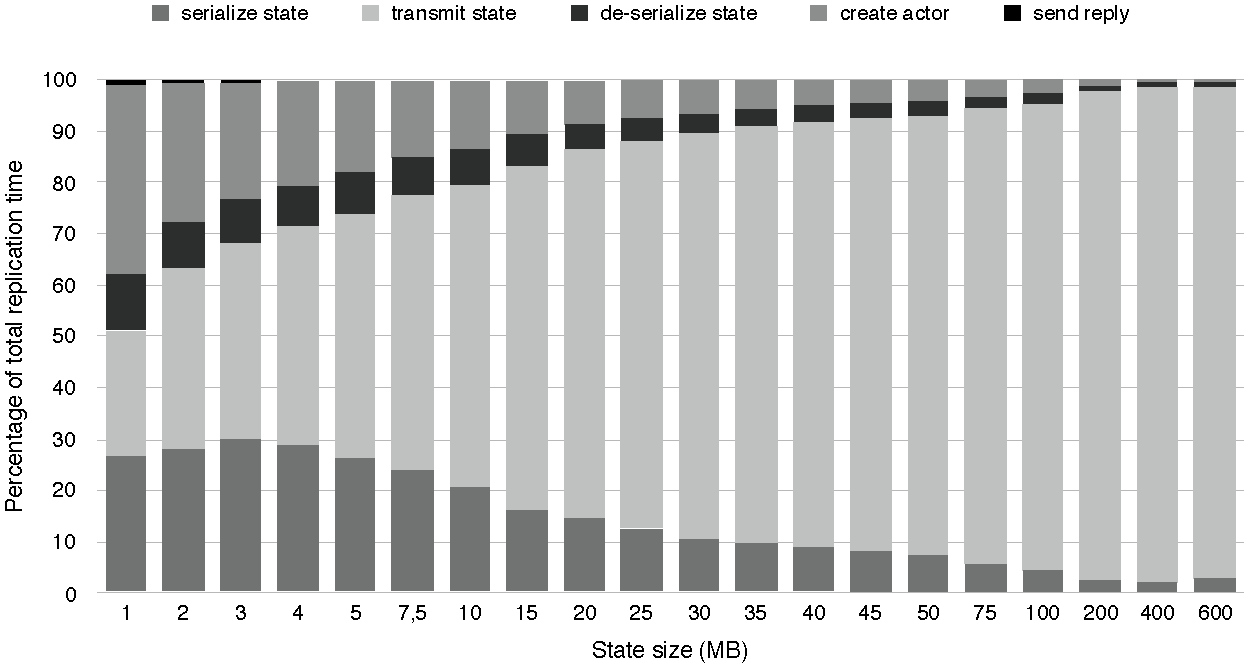
\includegraphics[scale=0.5]{images/results/replication_time/laptop_parts_variable.pdf} 
\caption{Result for test~\ref{sec:eval_repl_time}. Laptop to laptop, increased variable size} \label{fig:replication_time_parts_laptop_variable}
\end{figure}

\begin{figure}[hbt!]
\centering
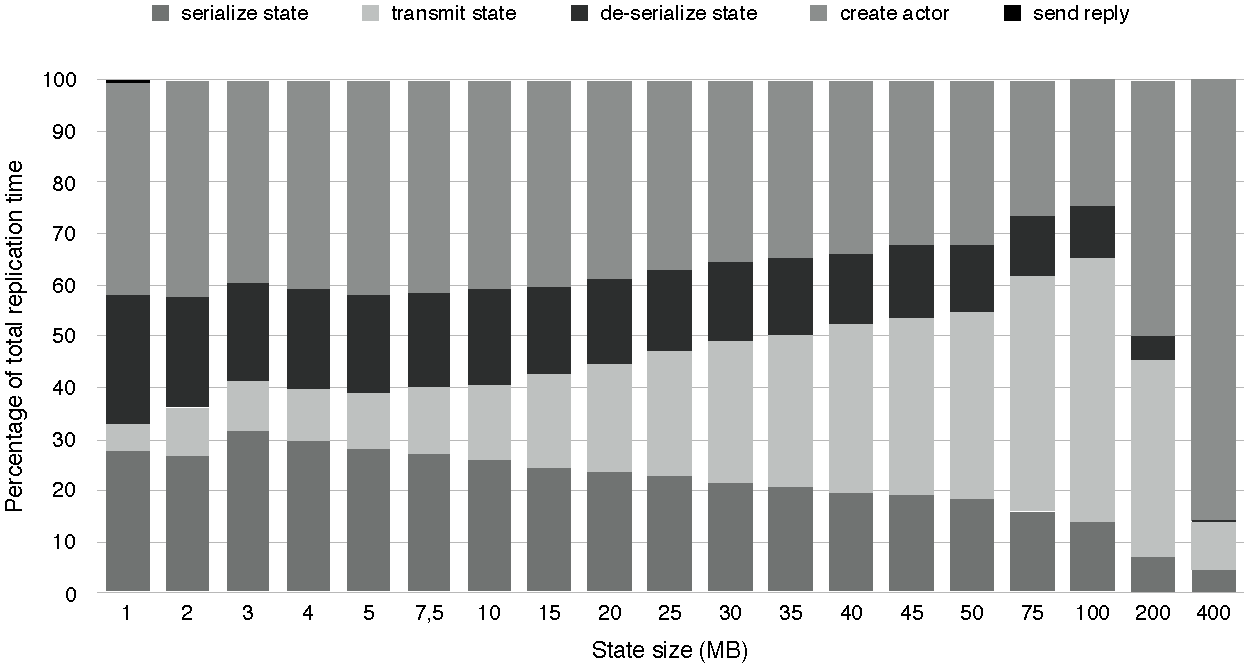
\includegraphics[scale=0.5]{images/results/replication_time/laptop_parts_queue.pdf} 
\caption{Result for test~\ref{sec:eval_repl_time}. Laptop to laptop, increased queue size.} \label{fig:replication_time_parts_laptop_queue}
\end{figure}

\subsubsection*{Results - replication time variance}
For 1, 50 and 100 MB the replication time was measured 100 times. The variance of the replication times was very small. \Cref{table:replication_time_variation_variable} and \cref{table:replication_time_variation_queue} show the average replication time, the standard deviation, and the standard deviation in percentage for these state sizes when increasing the variable's size, and the size of the queue respectively.
 
 \begin{table}[h!]
	\begin{center}
	\begin{tabular}{| c | c | c | c | c |}
	 \hline
	 replicating from/to & state size (MB) & $\mu$ & $\sigma$ & RSD \\
	 \hline		%TODO values
	  server/server & 1 & 0.041 & 0.001 & 0.024 \\
	  server/server & 50 &  5.523 &  0.056 & 0.010 \\
	  server/server & 100 &  20.177 & 0.385 & 0.019 \\
	  laptop/laptop & 1 & 0.087 & 0.020 & 0.229 \\
	  laptop/laptop & 50 & 10.617 & 1.210 & 0.114 \\
	  laptop/laptop & 100 & 34.019 & 1.412 & 0.041 \\
	   \hline
	\end{tabular}
	 \caption{Result for test~\ref{sec:eval_repl_time}. Average replication time in seconds ($\mu$), standard deviation ($\sigma$), and the relative standard deviation (RSD) for state sizes 1, 50 and 100 MB, where the state size was increased by increasing the size of one of the actor's variables.}
	 \label{table:replication_time_variation_variable}
	 \end{center}
 \end{table}
 
\begin{table}[h!]
	\begin{center}
	\begin{tabular}{| c | c | c | c | c |}
	 \hline
	 replicating from/to & state size (MB) & $\mu$ & $\sigma$ & RSD \\
	 \hline		%TODO values
	  server/server & 1 & 0.251 & 0,008 & 0,032 \\
	  server/server & 50 & 16,547 & 0.256 & 0,015 \\
	  server/server & 100 & 42.555 & 0.414 & 0,010 \\
	  laptop/laptop & 1 & 0.348 & 0.043 & 0.124 \\
	  laptop/laptop & 50 & 19.075 & 0.299 & 0.016 \\
	  laptop/laptop & 100 & 50.893 & 1.066 & 0.021 \\
	   \hline
	\end{tabular}
	 \caption{Result for test~\ref{sec:eval_repl_time}. Average replication time in seconds ($\mu$), standard deviation ($\sigma$), and the relative standard deviation (RSD) for state sizes 1, 50 and 100 MB, where the state size was increased by increasing the size of the actor's port queue.}
	 \label{table:replication_time_variation_queue}
	 \end{center}
 \end{table}
 

\subsection{Ensuring a certain reliability level} \label{sec:eval_rel_level}
In this experiment, each runtime was given a MTBF of 20 seconds.

After the application was started, the reliability level of the nodes on which replicas were running was periodically measured. The desired level of reliability for the producing actors were 0.98.

The test was considered successful if the average reliability level during the duration of the test exceeded 0.98. %TODO this is actually weird since we do not guarantee the average level is above XXX

\subsubsection*{Results}
%TODO include info about replication time
The experiment ran for 5 minutes, and \cref{fig:exp_reliability_level} shows how the reliability vary during this period. The average reliability for the duration of the whole test was 0.996, clearly above the desired level of 0.98.

As shown in the figure, the reliability was lower in the beginning of the test. This is due the lack of failure data for nodes, therefore assuming the default value for the MTBF of 10 seconds. As the nodes starts failing, the system learns their actual MTBF, which in the test was 20 seconds. Every drop in reliability corresponds to a failure of one of the nodes on which a replica is executing.

%TODO this needs to be updated? Not the latest?
\begin{figure}[!hbt]
\centering
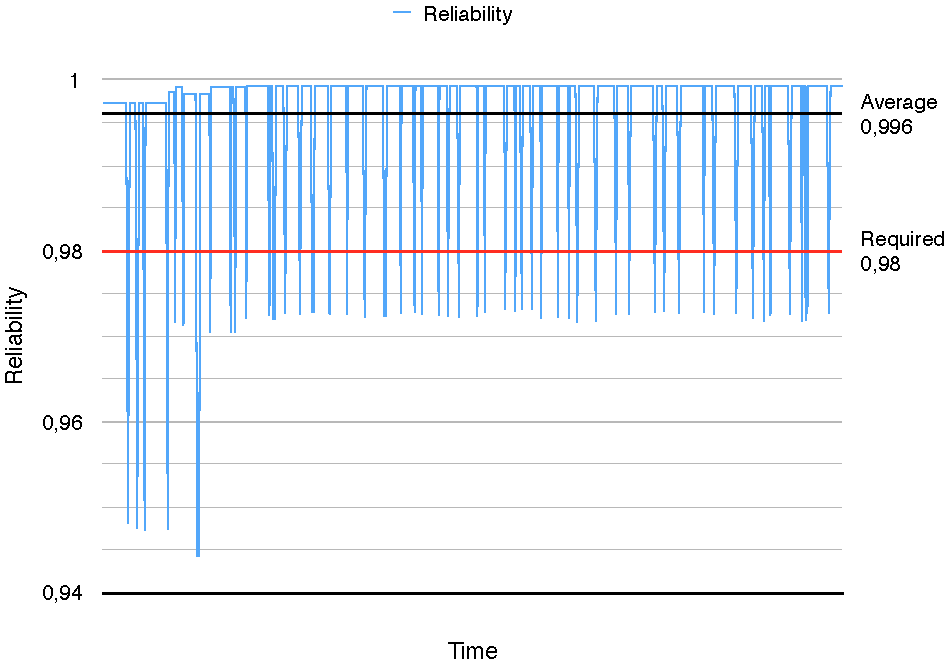
\includegraphics[scale=0.5]{images/results/reliability.pdf}
\caption{Result for test~\ref{sec:eval_rel_level}. Reliability over time in a system with failing nodes.} \label{fig:exp_reliability_level}
\end{figure}

\subsection{Optimal number of replicas}
\subsubsection{Chosing the most reliable} \label{sec:eval_opt_nbr_replicas}
In this experiment, the MTBF for the various runtimes varied. The mean values given to the different runtimes are presented in \cref{table:exp_nodes_means}. 

\begin{table}[h]
	\begin{center}
	\begin{tabular}{| c | c |}
	 \hline
	 node & MTBF (s) \\
	 \hline		
	  $dave_1$ & 7.5 \\
	  $dave_2$ & 7.5 \\
	  $tim_1$ & 7.5 \\
	  $tim_2$ & 7.5 \\
	  $kevin_1$ & 15 \\
	  $kevin_2$ & 15 \\
	  $mark_1$ & 15 \\
	  $mark_2$ & 40 \\
	  $jerry_1$ & 40 \\
	  $jerry_2$ & 40 \\
	   \hline
	\end{tabular}
	 \caption{Mean-time-between-failures for the eight unstable runtimes in the experiment~\ref{sec:eval_opt_nbr_replicas}.}
	 \label{table:exp_nodes_means}
	 \end{center}
 \end{table}


After the application was started, the reliability level of the nodes on which replicas were running was periodically measured. The desired level of reliability for the producing actors were 0.999.

The test was considered successful if the number of replicas used decreased over time, as the system learned the actual MTBF for the nodes, and consequently more reliable nodes could be chosen. Furthermore, for the test to be successful, the average reliability for the duration of the test should exceed 0.999. %TODO also weird since we do not guarantee the average is above the required.

\subsubsection*{Results}
%TODO include info about replication time
%TODO
The experiment ran for 5 minutes, and~\cref{fig:exp_opt_replicas_total} shows the number of replicas over time, while~\cref{fig:exp_opt_replicas_MTBF_30},~\cref{fig:exp_opt_replicas_MTBF_15}, and~\cref{fig:exp_opt_replicas_MTBF_75} show the number of replicas per node over time.

As shown in the figures, the number of replicas decreased over time, from three replicas at the start of the test, to later only two. Furthermore,~\cref{fig:exp_opt_replicas_MTBF_30} shows that the more reliable nodes, $mark_2$, $jerry_1$, and $jerry_2$, were chosen more often than the less reliable ones, shown in~\cref{fig:exp_opt_replicas_MTBF_30} and~\cref{fig:exp_opt_replicas_MTBF_75}.

\begin{figure}[!hbt]
\centering
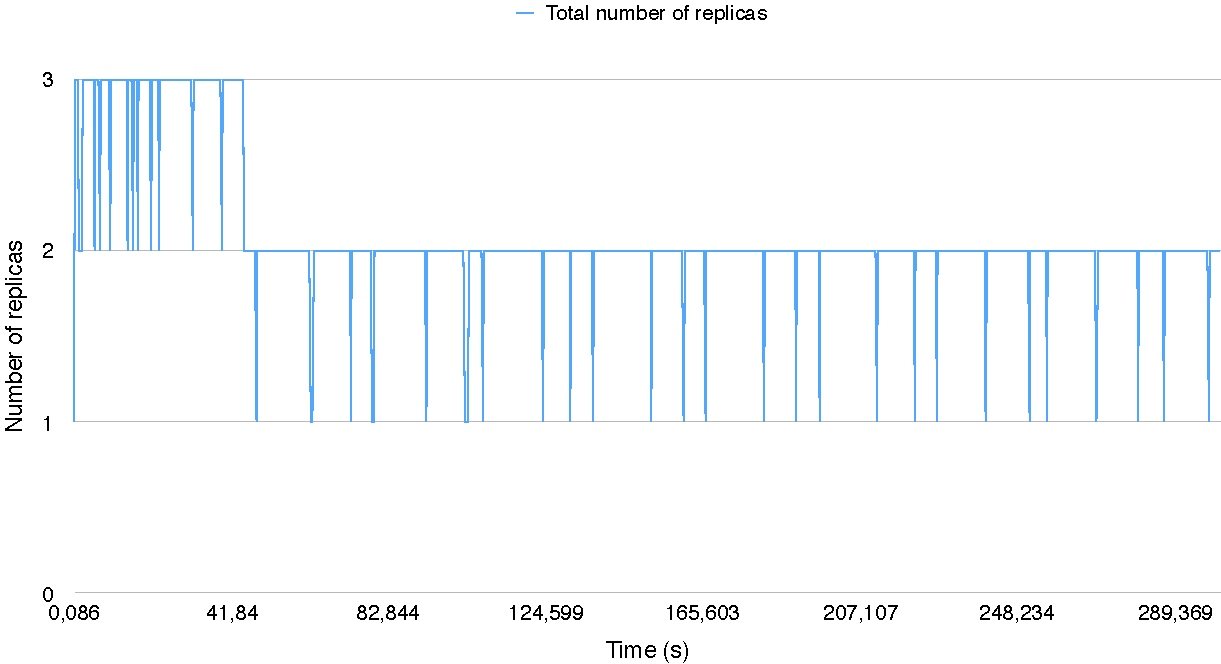
\includegraphics[scale=0.5]{images/results/optimal_replicas/total.pdf}
\caption{Result for test~\ref{sec:eval_opt_nbr_replicas}. Total number of replicas.} \label{fig:exp_opt_replicas_total}
\end{figure}

\begin{figure}[!hbt]
\centering
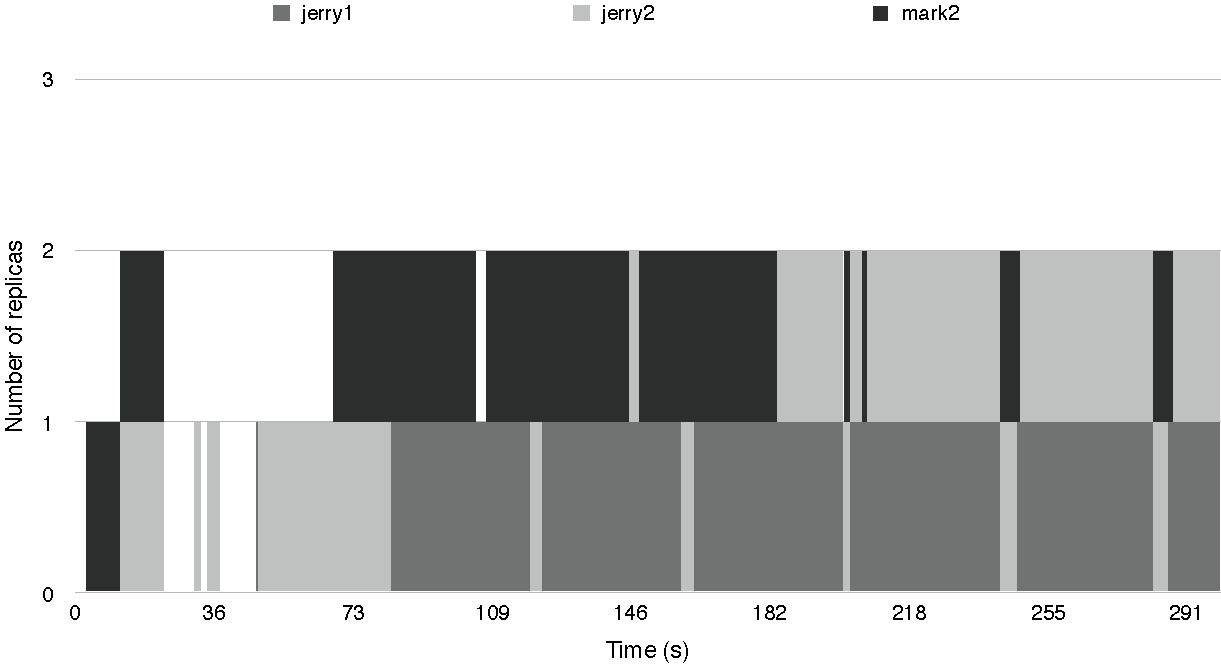
\includegraphics[scale=0.5]{images/results/optimal_replicas/MTBF_30.pdf}
\caption{Result for test~\ref{sec:eval_opt_nbr_replicas}. Number of replicas per node, for the three nodes with a MTBF of 30 seconds.} \label{fig:exp_opt_replicas_MTBF_30}
\end{figure}

\begin{figure}[!hbt]
\centering
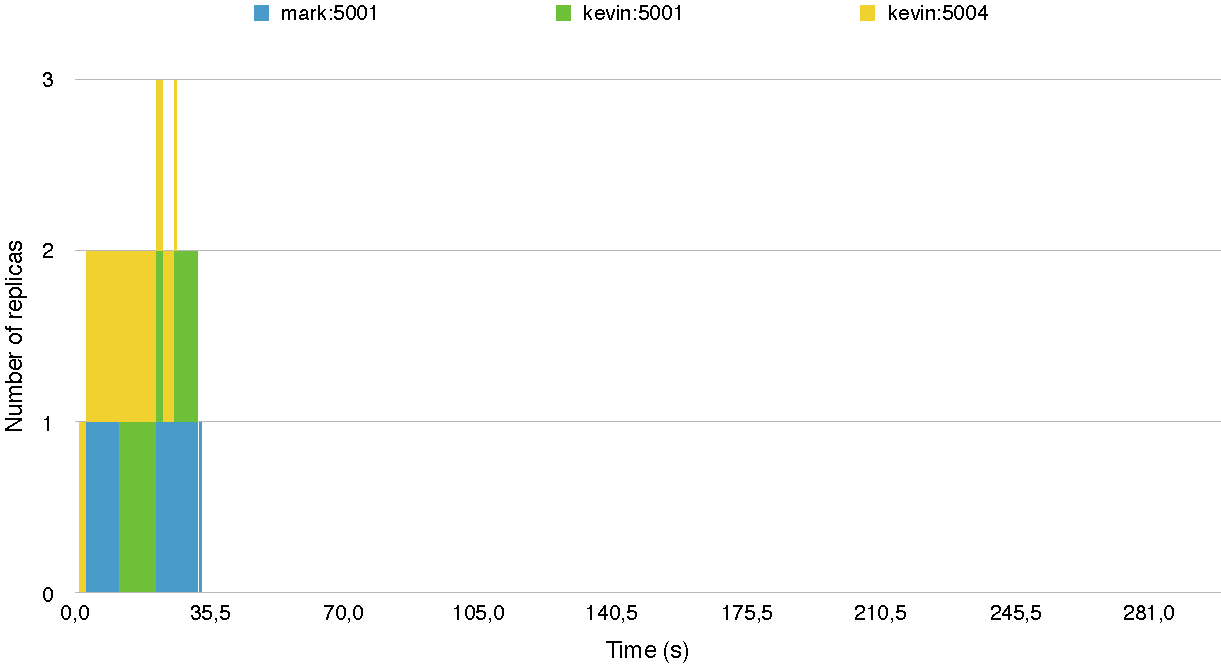
\includegraphics[scale=0.5]{images/results/optimal_replicas/MTBF_15.pdf}
\caption{Result for test~\ref{sec:eval_opt_nbr_replicas}. Number of replicas per node, for the three nodes with a MTBF of 15 seconds.} \label{fig:exp_opt_replicas_MTBF_15}
\end{figure}

\begin{figure}[!hbt]
\centering
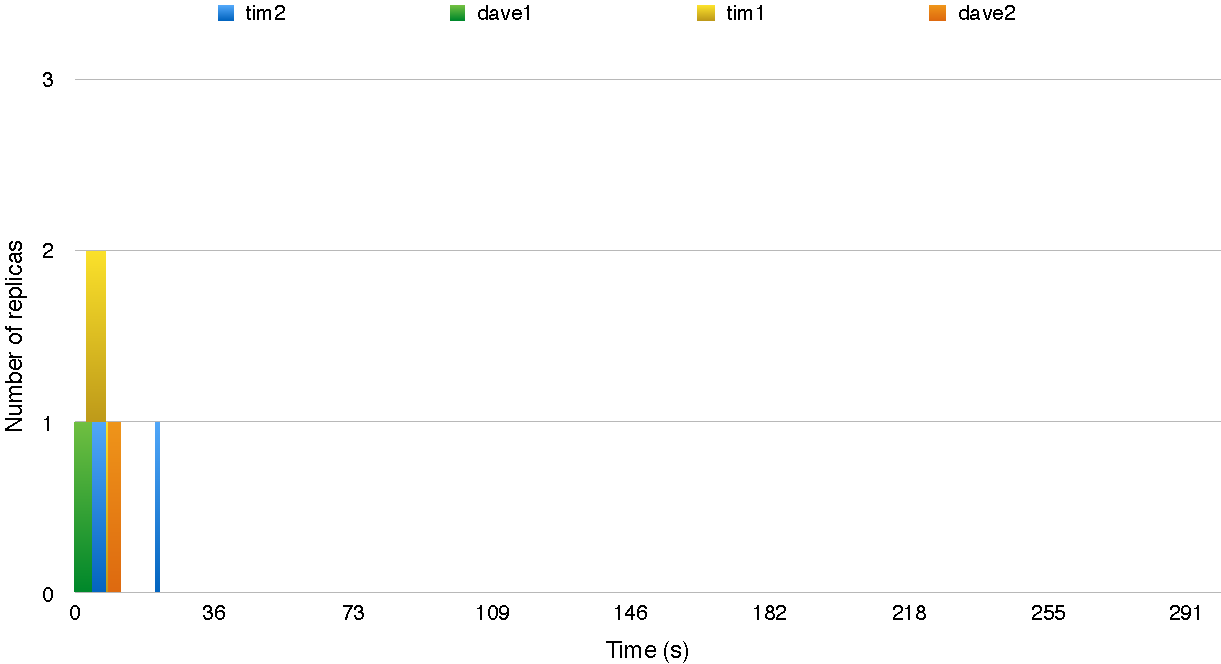
\includegraphics[scale=0.5]{images/results/optimal_replicas/MTBF_75.pdf}
\caption{Result for test~\ref{sec:eval_opt_nbr_replicas}. Number of replicas per node, for the four nodes with a MTBF of 7.5 seconds.} \label{fig:exp_opt_replicas_MTBF_75}
\end{figure}

\subsubsection{Optimal replicas}
\label{sec:eval_opt_nbr_replicas_2}
In order to show that the system automatically reduces the number of replicas in case more reliable nodes are available, an experiment was conducted in which five computing nodes were used. Two of these nodes were given a MTBF of 25 seconds, while the other three did not fail. Since those three nodes did not fail, the system used the default MTBF of 10 seconds. Despite not failing, the system considered them less reliable than the two failing nodes with MTBF of 25 seconds. The reason for not killing those three nodes were simply in order to show that the system automatically reduces the number of replicas, not only when a node fails. The MTBF for the nodes used in this experiment are shown in \cref{table:exp_nodes_means}.

The required reliability in the experiment was set to 0.999. This results in that as long as the two reliable nodes are available, only two replicas are needed, but if one of them or both are dead, three replicas are needed to reach the required reliability. Finally, a delay of 5 seconds were used between killing and restarting nodes \emph{kevin} and \emph{jerry}.


\begin{table}[h]
	\begin{center}
	\begin{tabular}{| c | c |}
	 \hline
	 node & MTBF (s) \\
	 \hline		
	  $dave$ & 10 \\
	  $tim$ & 10 \\
	  $mark$ & 10 \\
	  $kevin$ & 25 \\
	  $jerry$ & 25 \\
	   \hline
	\end{tabular}
	 \caption{Mean-time-between-failures for the five runtimes in the experiment~\ref{sec:eval_opt_nbr_replicas_2}.}
	 \label{table:exp_nodes_means_2}
	 \end{center}
 \end{table}


\subsubsection*{Results}
%TODO include info about replication time
The test ran for 5 minutes. As mentioned, the default MTBF is 10 seconds when no failure data is known for a node. This means when the more unreliable nodes have failed twice, their MTBF will be 25 seconds, higher than the default value. But before the reliable nodes have failed twice, their MTBF will be 10 seconds. This is why there is a period during which none of the reliable nodes are given any replicas. After their seconds failure however, it is known that they are actually more reliable than the other ones, why they are then given replicas.

\begin{figure}[!hbt]
\centering
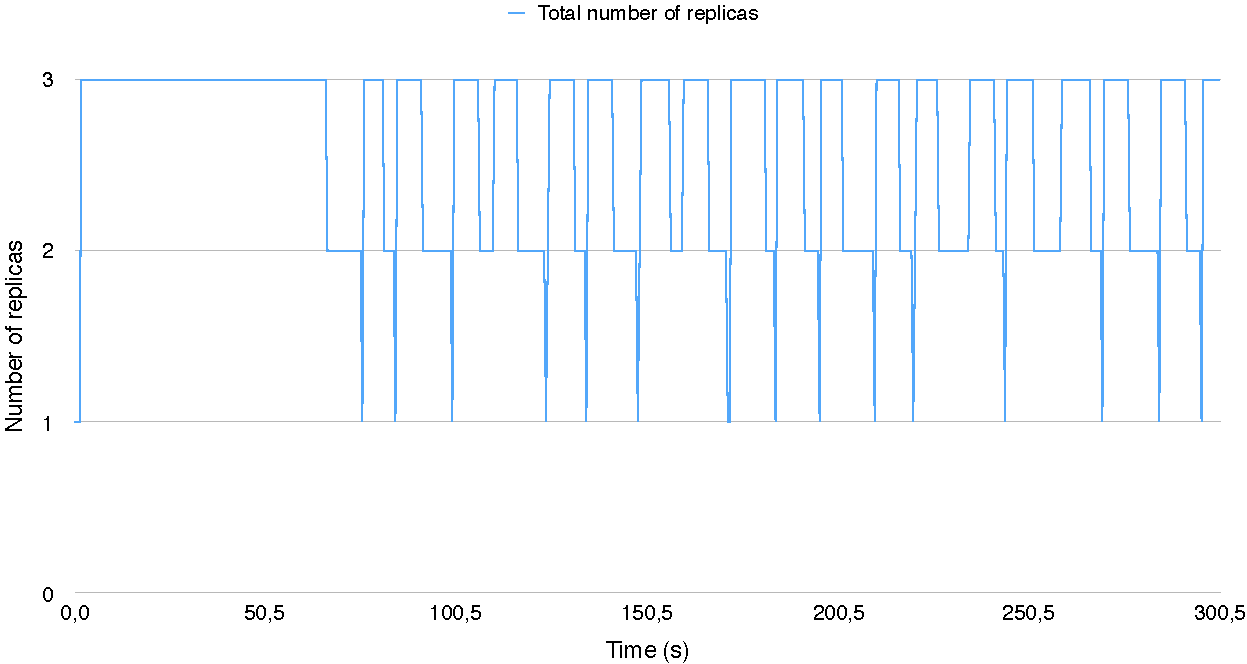
\includegraphics[scale=0.5]{images/results/optimal_replicas/2/total.pdf}
\caption{Result for test~\ref{sec:eval_opt_nbr_replicas_2}. Total number of replicas.} \label{fig:exp_opt_replicas_total_2}
\end{figure}

\begin{figure}[!hbt]
\centering
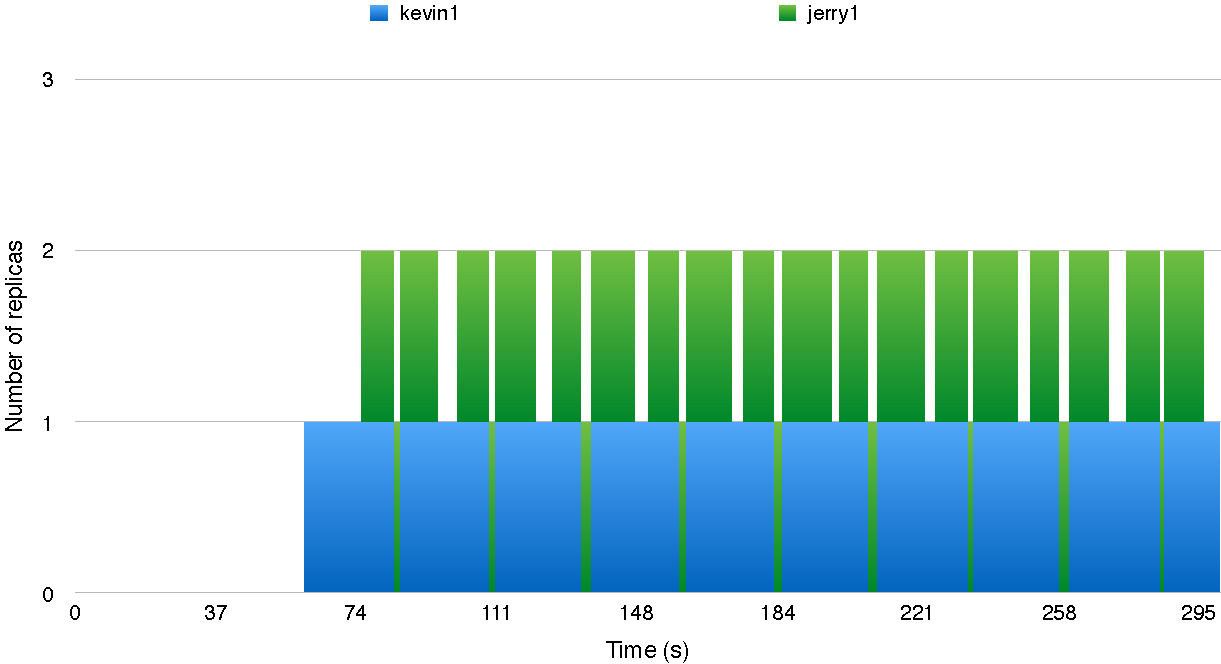
\includegraphics[scale=0.5]{images/results/optimal_replicas/2/MTBF_25.pdf}
\caption{Result for test~\ref{sec:eval_opt_nbr_replicas_2}. Number of replicas per node, for the two nodes with a MTBF of 25 seconds.} \label{fig:exp_opt_replicas_MTBF_25_2}
\end{figure}

\begin{figure}[!hbt]
\centering
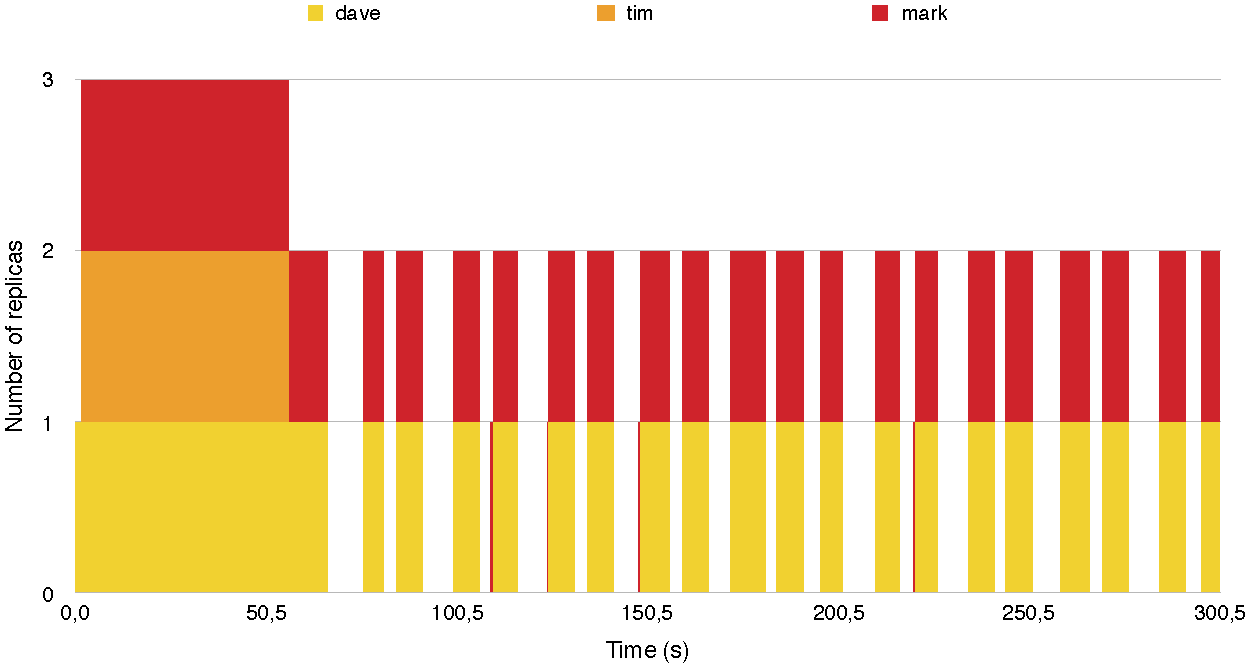
\includegraphics[scale=0.5]{images/results/optimal_replicas/2/MTBF_10.pdf}
\caption{Result for test~\ref{sec:eval_opt_nbr_replicas_2}. Number of replicas per node, for the three nodes which were not killed, and therefore were assumed to have a MTBF of 10 seconds.} \label{fig:exp_opt_replicas_MTBF_10_2}
\end{figure}


\subsection{Self-adaptive reliability model} \label{sec:eval_adaptive_rel_model}
%TODO the mean-time-between-failure does not vary, really... must rephrase this sentence
In this experiment, the MTBF for the various nodes varied over time, following a $sinus-curve$. The pseudo-random numbers for the nodes followed a normal distribution with mean 25 and standard deviation of 1. However, the time to sleep between failures were calculated by~\ref{eq:eval_sleep_time}. This means the time between failures varied between 5 and 45 seconds. The required reliability was set to 0.99999. This value was chosen so that the number of replicas needed would vary between 3 and 5, depending on the current state of the system.

%TODO how long should before we're back? 60 sec?
\begin{equation} \label{eq:eval_sleep_time}
T_{sleep} = t_i + 20 * \sin{(2\*\pi\*T_{elapsed} / 300)}
\end{equation}

Where $t_i$ are the numbers following a normal distribution with mean 25 and standard deviation of 1, and $T_{elapsed}$ is the total elapsed time for the test. Given $t_i=25$, \cref{fig:eval_sleep_time} in~\cref{appendix:figures} shows how the actual time to sleep varies over time.

The process of killing nodes therefore differed from~\cref{alg:simulating_node_failures}. How nodes were killed and restarted in this experiment is shown in~\cref{alg:simulating_node_failures_sinus}.

\begin{algorithm} 
	\caption{Simulating node failures} \label{alg:simulating_node_failures_sinus}
	\begin{algorithmic}[1]
	\State $T_{start}\gets$ current time
	\While {$true$}
		\State
		\Call{start runtime}{}
		\State $T_{now}\gets$ current time
		\State $T_{elapsed}\gets T_{start}-T_{now}$
		\State {$t_{s}\gets \mathcal{N} (MTBF,1) + 20 * \sin{(2\*\pi\*T_{elapsed} / 300)}$}
		\State
		\Call{sleep $t_{s}$}{}
		\State
		\Call{kill runtime}{}
	\EndWhile
	\end{algorithmic}
\end{algorithm}

The test was considered successful if the number of replicas used increased as the time between failures decreased for the various nodes, after which it increased as the time between failures increased.

\subsubsection*{Results}
The test ran for 30 minutes. \Cref{fig:eval_self_adaptive_rel} shows how the number of replicas varied over time, and~\cref{fig:eval_self_adaptive_node_rels} shows how the calculated reliability for the various nodes vary over time. 

\begin{figure}[!hbt]
\centering
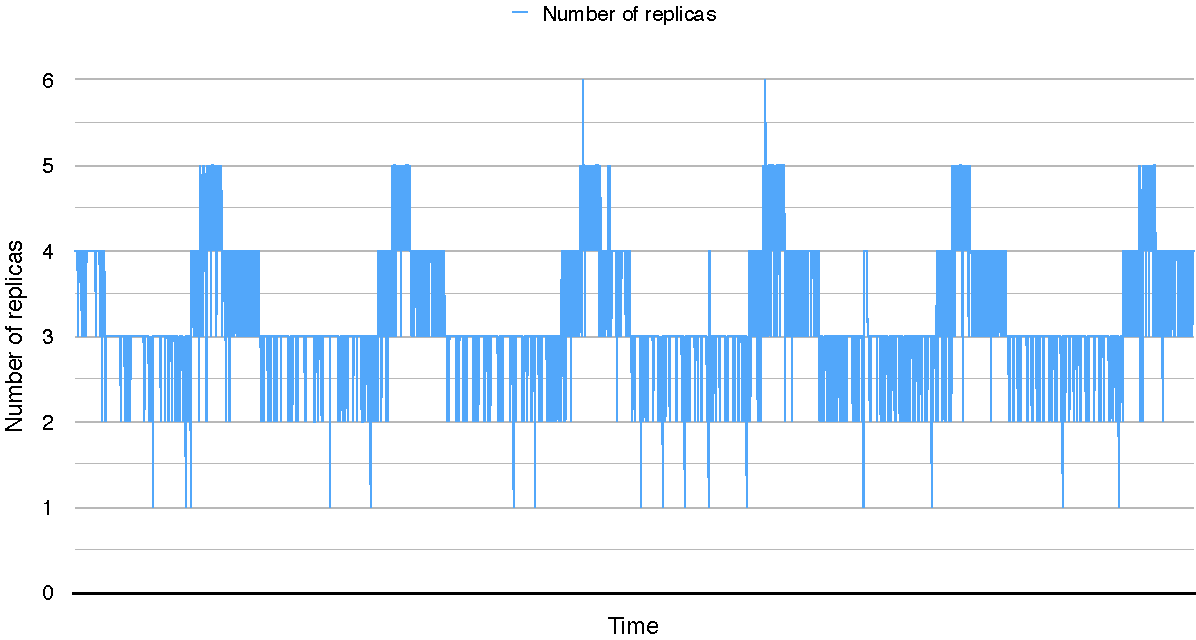
\includegraphics[scale=0.5]{images/results/self_adaptive_replicas.pdf}
\caption{Result for test~\ref{sec:eval_adaptive_rel_model}. Reliability over time with failing nodes and varying time between failures.} \label{fig:eval_self_adaptive_rel}
\end{figure}

\begin{figure}[!hbt]
\centering
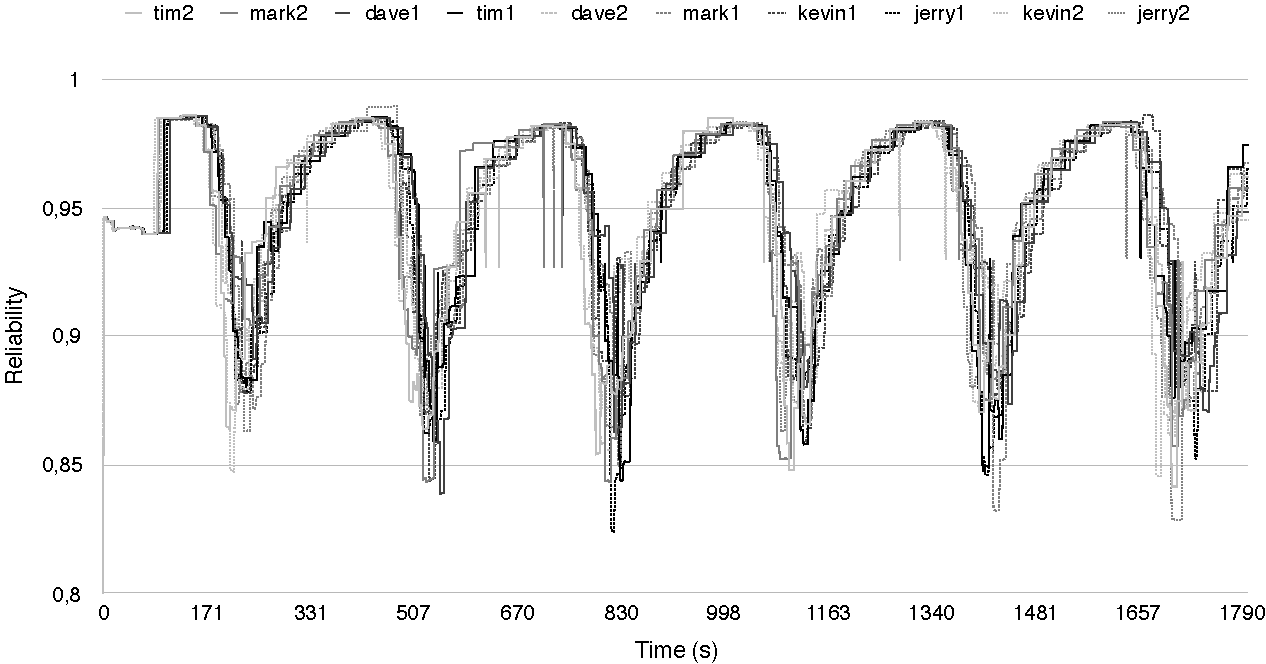
\includegraphics[scale=0.5]{images/results/self_adaptive_node_rels.pdf}
\caption{Result for test~\ref{sec:eval_adaptive_rel_model}. Reliability over time with failing nodes and varying time between failures.} \label{fig:eval_self_adaptive_node_rels}
\end{figure}

\subsection{Energy efficient for many applications} \label{sec:eval_energy_efficient}
%TODO 5 applications and 3 replicas or tvartom?
In this experiment, 5 applications were started instead of only one. The applications were identical, described in~\cref{sec:eval_application}, with a required reliability of 0.99999. 

Two runtimes were started on each server. The MTBF of the runtimes were the same as for experiment~\cref{sec:eval_opt_nbr_replicas}, and shown in~\cref{table:exp_nodes_means}.

%TODO this section needs work.
When the MTBF for the runtimes is known, only two replicas per application is needed to reach above the required reliability, while three replicas are needed when it's unknown. Since the replicas are placed on the most reliable nodes, each application would have its replicas on the same nodes, i.e. the most reliable ones. Therefore, theoretically only two nodes would be needed when the MTBF is known, since each applications' two replicas would be placed on the two most reliable nodes. The test is therefore considered successful if the nodes used at any time were kept to a minimum, which theoretically would be two when the MTBF is known.

\subsubsection*{Results}
The test ran for 5 minutes, and \cref{fig:eval_energy_efficient_total} shows the total number of nodes used at any time. As shown in the figure, the number of nodes used varies between two to three for the most time, until after about two minutes, after which only two nodes are needed most of the time. Despite having 10 nodes, at most 4 were actually used to at any time.

\Cref{fig:eval_energy_efficient_mtbf_40}, \cref{fig:eval_energy_efficient_mtbf_15}, and \cref{fig:eval_energy_efficient_mtbf_75} show the number of actors running at the various nodes. Since the model does not place two replicas of the same task on the same node, the nodes had at most 5 actors, one replica per application, at any time.

\begin{figure}[!hbt]
\centering
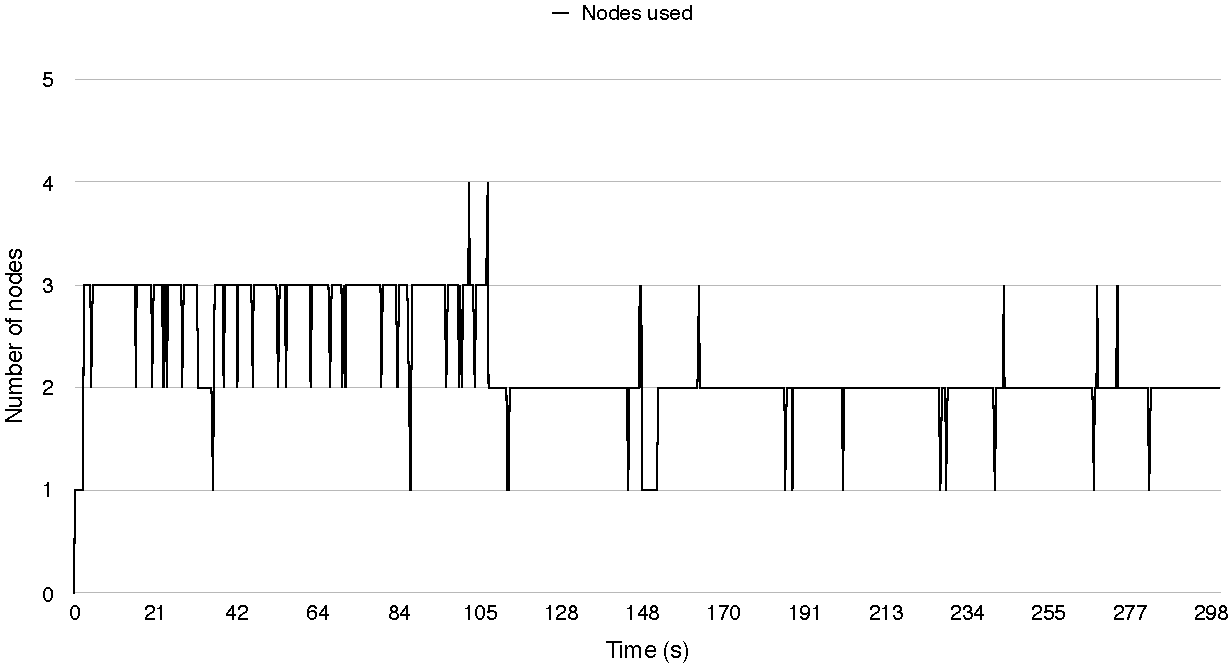
\includegraphics[scale=0.5]{images/results/energy_efficient/total.pdf}
\caption{Result for test~\ref{sec:eval_energy_efficient}. Number of nodes used.} \label{fig:eval_energy_efficient_total}
\end{figure}

\begin{figure}[!hbt]
\centering
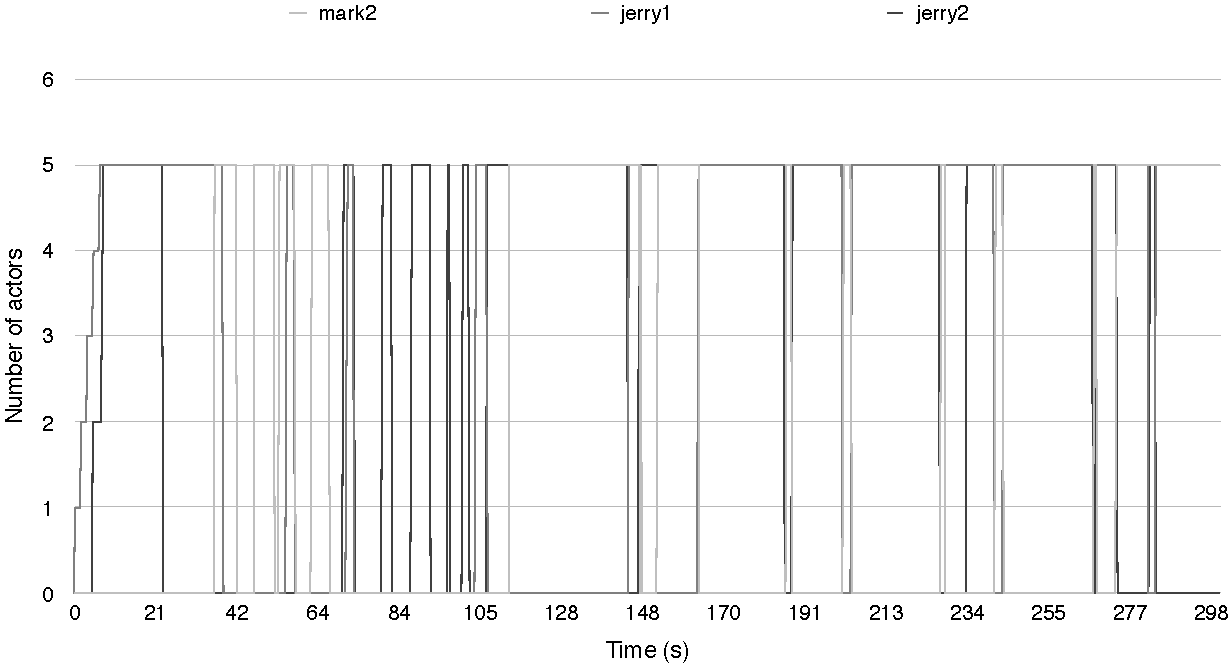
\includegraphics[scale=0.5]{images/results/energy_efficient/MTBF_40.pdf}
\caption{Result for test~\ref{sec:eval_energy_efficient}. Number of actors per node, for the three nodes with a MTBF of 40 seconds.} \label{fig:eval_energy_efficient_mtbf_40}
\end{figure}

\begin{figure}[!hbt]
\centering
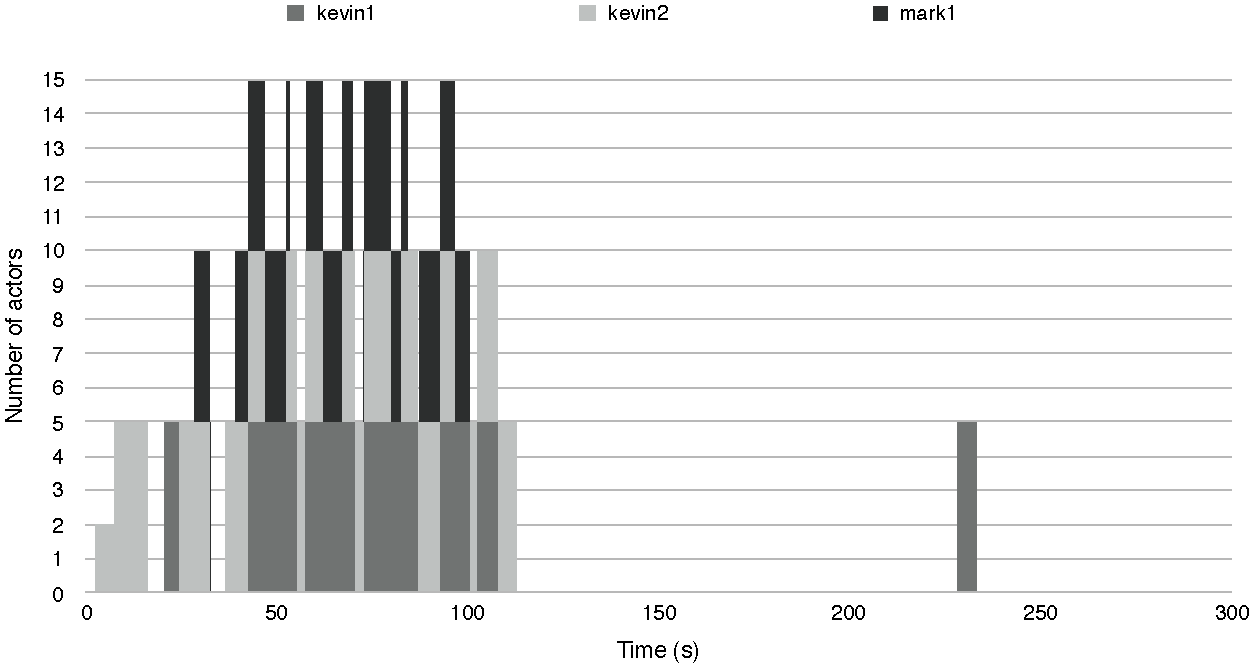
\includegraphics[scale=0.5]{images/results/energy_efficient/MTBF_15.pdf}
\caption{Result for test~\ref{sec:eval_energy_efficient}. Number of actors per node, for the three nodes with a MTBF of 15 seconds.} \label{fig:eval_energy_efficient_mtbf_15}
\end{figure}

\begin{figure}[!hbt]
\centering
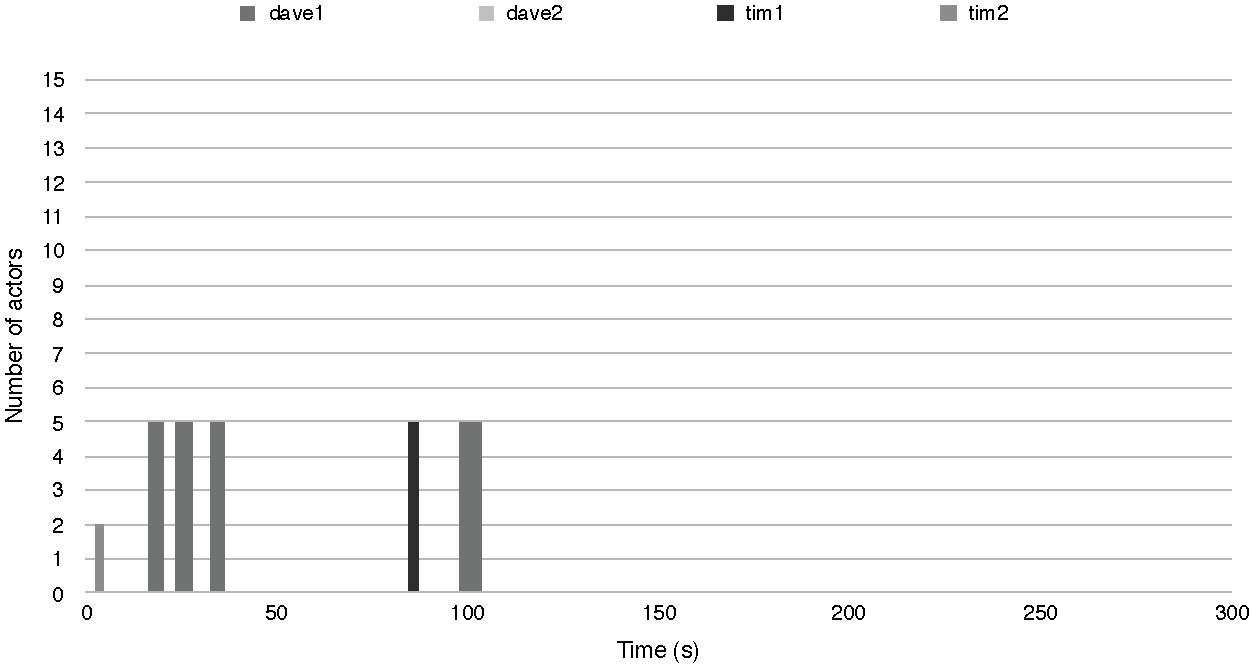
\includegraphics[scale=0.5]{images/results/energy_efficient/MTBF_75.pdf}
\caption{Result for test~\ref{sec:eval_energy_efficient}. Number of actors per node, for the three nodes with a MTBF of 7.5 seconds.} \label{fig:eval_energy_efficient_mtbf_75}
\end{figure}

\subsection{Considering nodes' load} \label{sec:eval_replaceable_model}
Lastly, to show that the reliability model and selection of nodes to place replicas on are replaceable with more sophisticated algorithms, a test was conducted in which the system avoids placing replicas on nodes with a CPU usage above 15 percent. 

In this experiment, five nodes were used. Three of these nodes, \emph{Tim}, \emph{Mark}, and \emph{Jerry}, had a MTBF of 10 seconds, and two, \emph{Dave} and \emph{Kevin}, had a MTBF of 40 seconds. Furthermore, the load on \emph{Kevin} was increased after a while by starting dummy jobs simply to consume CPU resources, and was later decreased again. The required reliability in this test was set to 0.999.

The test was considered successful if, despite being one of the more reliable nodes, the system avoided to place replicas on \emph{Kevin}, during the time its load was above the threshold of 15 percent.

\subsubsection*{Results}
The test ran for 5 minutes. \Cref{fig:eval_replaceable_model_usages} shows the CPU usage for the various nodes. \Cref{fig:eval_replaceable_model_loaded} and \cref{fig:eval_replaceable_model_unloaded} show the number of replicas for \emph{Kevin} and the other nodes during the test.

\Cref{fig:eval_replaceable_model_loaded} clearly shows no replica was placed on \emph{Kevin} during the time its load exceeded the threshold of 15 percent. This means our model is general and key components such as calculating the reliability of a node as well as sorting the available nodes may be replaced. 

\begin{figure}[!hbt]
\centering
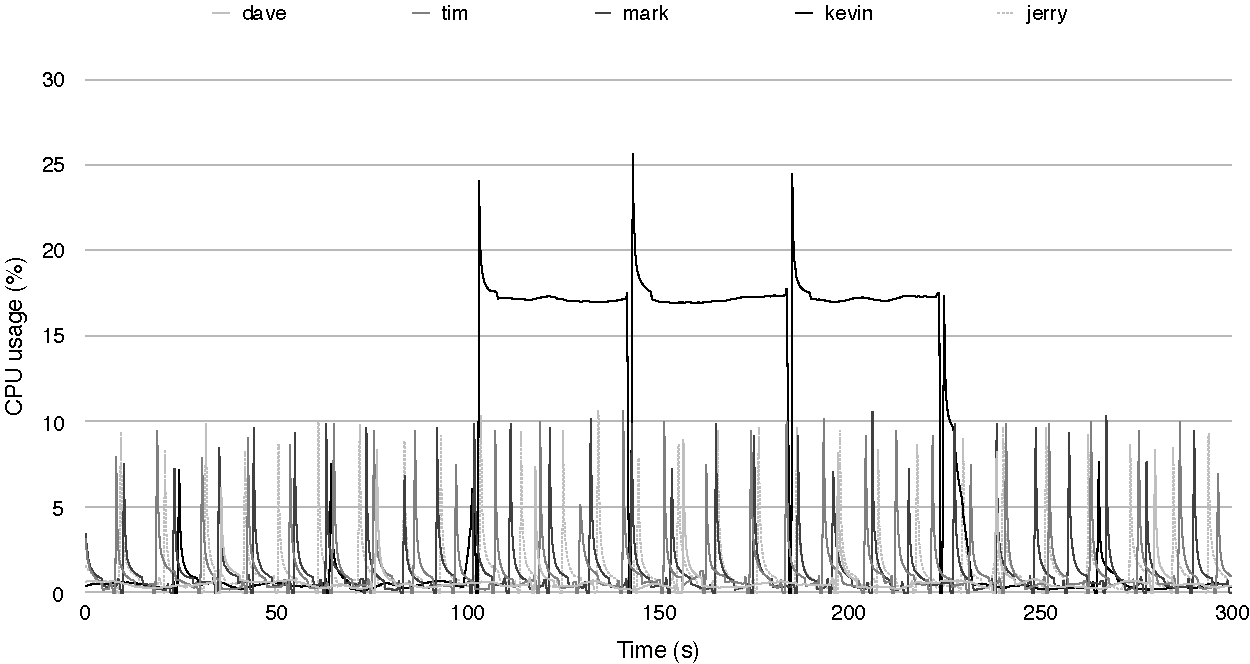
\includegraphics[scale=0.5]{images/results/loads/usages.pdf}
\caption{CPU usages in percent for the nodes used in test~\ref{sec:eval_replaceable_model}.} \label{fig:eval_replaceable_model_usages}
\end{figure}

\begin{figure}[!hbt]
\centering
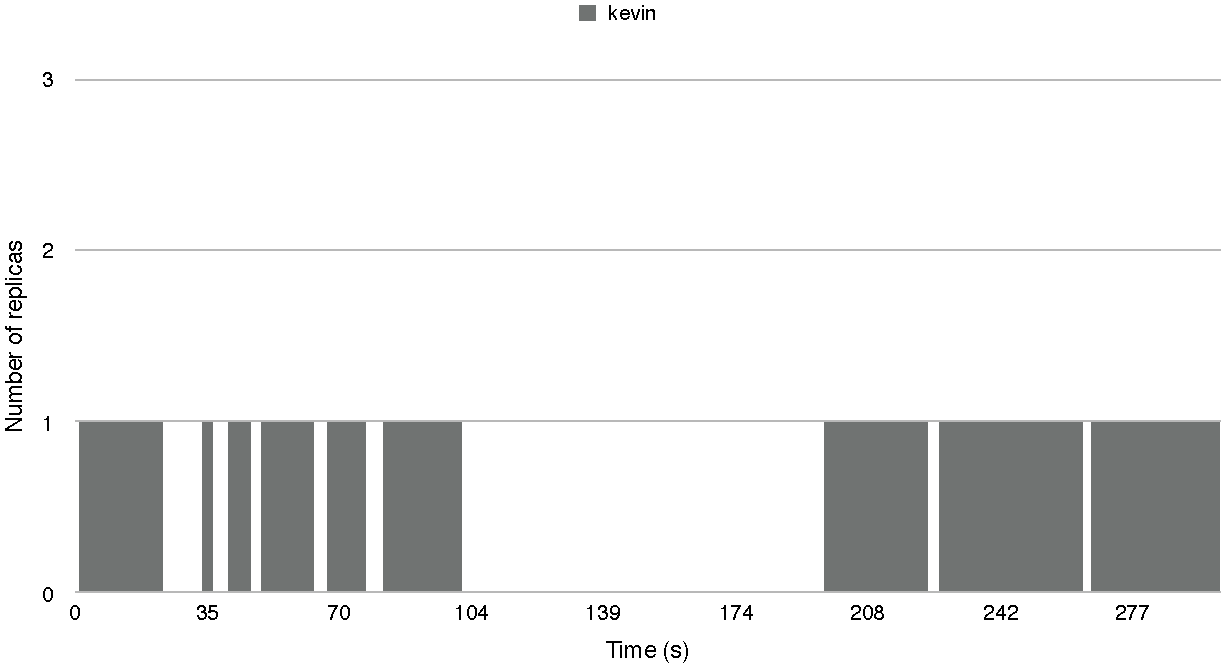
\includegraphics[scale=0.5]{images/results/loads/loaded.pdf}
\caption{Result for test~\ref{sec:eval_replaceable_model}. The number of replicas over time for node \emph{Kevin}.} \label{fig:eval_replaceable_model_loaded}
\end{figure}

\begin{figure}[!hbt]
\centering
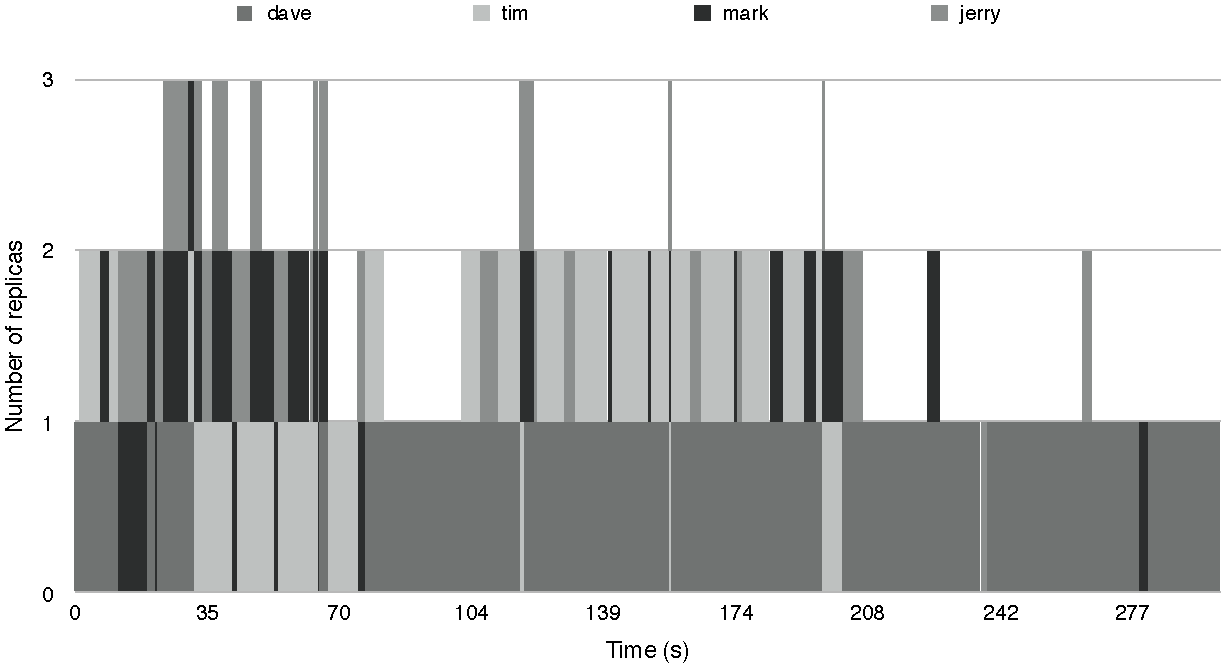
\includegraphics[scale=0.5]{images/results/loads/unloaded.pdf}
\caption{Result for test~\ref{sec:eval_replaceable_model}. The number of replicas per node for \emph{Tim}, \emph{Mark}, \emph{Jerry}, and \emph{Dave}.} \label{fig:eval_replaceable_model_unloaded}
\end{figure}

\chapter{Discussion} \label{ch:discussion}
%TODO
Since we update the reliability of a node after failure's happen ... if a node start's dying more often, the mtbf used is "a little behind"... EDIT ME.

%TODO
\iffalse
Större drag, vad kan vi få ut av alla experimenten?
Hur mycket kan vi lite på resulaten?
Är det worst-case/best-case?
Kommer det bara bli bättre/snabbare med tiden?
Generalla slutsater
Vi kan ej generalisera våra resultat. typ.
\fi

When using a fail-stop fault model (see \cref{subsub:background_fail_stop}), we assume that when a node dies all other nodes are aware of this. This is clearly limiting, as in the case of a link failure. Assume we have three nodes $A$, $B$ and $C$ and there is one replica on $A$ and one on $B$. In case of a link failure between $A$ and $B$, $A$ will assume that $B$ has failed and vice versa and both will ask the node with highest id to replicate the lost actors. If $C$ has the highest id of all three then nothing will happen since $C$ is aware of the replicas on both $A$ and $B$. But if $A$ has the highest id it will send the replication request to itself and since it's not aware of that there is a running replica on $B$, it will replicate its actor to $C$. Thereafter we have an unnecessary high reliability and, from a system perspective, there is a unnecessary high impact on the network load.

Our limitations also excludes the possibility of tasks calculating incorrect results, which is the case when using a Byzantine fault model. Since already using active replication to ensure reliability, it would be trivial to extend it to use consensus techniques such as majority voting or \emph{k-modular redundancy} in order to extend the reliability definition to also include that the job calculates the correct result.
\\

%\subsubsection{Replaceable reliability model}
%TODO is this more suitable in discussion perhaps?
\Cref{alg:scheduling} is designed to use the reliability model in a plugin fashion, namely by calling~\cref{func:calc_reliability}. This allows for easily replacing the reliability model without changing the algorithm itself.

Furthermore, determining which nodes to prefer when selecting where to place new replicas is also an external function call. In our case, the available nodes are sorted after reliability, see~\cref{func:get_available_nodes}. Also this function could be replaced without changing the algorithm. One could for example exclude nodes where the load is above a given threshold.

When getting available nodes, sorted by reliability with the preferred nodes first, it is important to consider the current nodes. Since only considering node failures, and assuming statistically independent failures, it is important not to place two replicas on the same node. In addition, this is also important if one were to take more parameters into account. For example, one may not want to have several replicas in the same rack, as they would all fail if the rack's switch fails.

If we assume that the task replicas themselves may fail independent of each other and the computation they perform we could actually in some cases want to place two replicas on the same node. In this case the current nodes could be included when getting the available nodes.
\\

Since we minimize the number of replicas used for each application and place them on the most reliable nodes we consequently use the minimum amount of nodes overall. Let's say we have five different actors which all needs to be replicated in order to reach a required level of reliability. Due to their different state sizes they have different replication times and therefore needs a different number of replicas. Assume it requires three, four, four, five respectively five replicas for each of the five actors. Then our model will only use five nodes in total for all twentyone replicas since the most reliable nodes will have replicas of all actors. In a bigger interconnected net of nodes this gives rise to the possibility to extend our model with some sort of algorithm shutting down/starting unnecessary resources, saving energy and money.

Our primary objective is to ensure a certain level of reliability. By using active replication, we require a lot more resources, which puts an extra burden on the system. In addition, the extra load on the system may affect the execution time, thus decreasing task performance.

Our model is yet to be evaluated on highly unreliable system during extreme load. In this case, due to the unreliability of the system, the number of replicas needed to ensure the required reliability level will increase. This will further increase the system load, thereby decreasing the reliability of the system even further. This may turn into a vicious circle.

Our model ensures that the reliability is higher than the required as long as we don't experience a node failure. After a node failure and before the system has recovered (replicated the lost actors) the reliability is lower than the required. Our model does not guarantee that the average reliability is higher than the required, it depends on the relationship between the MTBF and the time it takes to replicate an actor.

The reliability is dependent on the replication time, which depends on the state of the task to replicate. The Calvin framework is only designed for light-weight IoT applications, thus not for applications where the actor state is several megabytes, and not optimized for this kind of work. Despite this, the experiments show that it takes less than one hour to replicate an actor with a state of 1 gigabyte. Assuming a mean-time-between-failures of one year (31536000 s), and an replication time of 1 hour (3600 s), having only two replicas still according to \cref{eq:task_reliability_3} gives a reliability of

\begin{equation*}
\begin{split}
R(3600) = e^{3600/31536000}\\
\\
R_{T}(3600) = 1 - \prod\limits_{k=1}^2 F_{k}(3600)\\
= 1 - \prod\limits_{k=1}^2 (1 - R(3600))\\
= 1 - (1 - e^{3600/31536000})^2\\
= 0.999999986302961
\end{split}
\end{equation*}

This means despite having a large replication time, a high reliability can be achieved by only having two replicas.

If our model is to be used in an environment where not all nodes are located within the same cluster, one must take into account that the replication time will be higher when replicating to a node in another cluster than within the same cluster.

Finally, since using a \emph{default MTBF} of nodes for which we have not yet experienced failure, our model is obviously limited, as this default value may be incorrect. To use in a real-world situation by a service provider, the reliability model must be extended. To cope with the MTBF, one could use past failure data from their cluster. Furthermore, the model should be extended to also take into account parameters like system load, link failures, etc. 

% Should we afford losing the most reliable node? According to definition rel = prob that we don't loose all OTHER nodes during a node failure. What if we dont have a node failure? Simulate one by not including the most reliable node in the calculations of rel.

%Mention that since we always place the replicas on the most reliable nodes our model uses the least amount of resources and are therefore energy efficient. Assume we have 100 actors that all need to be replicated. Then we use at most max(nbr_of replicas) nodes (asuming that we dont cross the max preferred level). 

\chapter{Future Work} \label{ch:future_work}
%TODO  move this paragraph
Since periodically monitoring the reliability, some machine learning technique would be beneficial. Instead of acting first when the reliability is below the desired value, one could predict when the reliability is about to decrease and take preventative measures.

To the best of our knowledge our model is the first of it's kind, due to its fully dynamic behavior. Therefore we had to limit our scope a lot and considering these limitations there is a lot of possible future work. Our model could be extended by considering more types of failures, e.g. link failure and soft failures (e.g. an actor dies but not the node or the actor produce an incorrect result). A consensus algorithm should be implemented in order to hamper the risk of using incorrect results. Link failures could, for instance be detected if the node responsible for replicating actors after a node failure awaits request from several nodes. If it only receives one node fail request among ten nodes its safe to assume that the node is still alive and the link to the requesting node has failed.

There are a lot of different kinds of failures which could be taken into account, see \cref{subsec:future_extended_model} for an extended reliability model.

Our model could also be extended with some sort of machine learning in order to predict future failures. In the case of a video service its likely that the system load is higher in the evening and therefore also the probability of a failure. By predicting these failures replicas an be created in advance, i.e. when the probability of failure reaches above a certain threshold.

In our experiments we have had only one actor to replicate on the lost node, in bigger systems with many actors on each node we get the complexity of choosing which actor to replicate first. A solution could be to have a criticality of each actor type and start replicating the most critical actor on the lost node. However, replication time is defined as the time it takes from that we start replicating actors at all after a node failure to that the actor is up and running, i.e. all actors replication times have the same start time. This will result in that the least critical actor will have the largest replication time and thereby being having the most amount of replicas. 
Another, perhaps better solution would be to replicate the actors with the biggest states first in order to achieve an uniformly distribution of the replication times as possible. We leave the investigation of which algorithm is the optimal to future work.

Furthermore, our model does not guarantee that the average of the actual reliability is above the required, it only aims at keeping the current reliability higher than the required. An solution to this would be to aim at keeping the current average reliability above the required. This is further described in \cref{subsec:future_extended_model}. 

%TODO
\iffalse
NOTES:
Replication impose extra burden on the system as additional resources are needed and computational power is wasted. By combining checkpointing techniques with active replication, the number of replicas needed could possible be decreased.(~\cite{adaptiveCheckPointAndRep} combines checkpointing and replication)
\\\\
Predict future failures - machine learning (many parameters could be taken into account), and when the probability of failure reaches above a certain threshold, the running tasks on that node could be migrated. A high reliability in failure prediction allows for fewer replicas to be needed.
\\\\
Implement consensus in Calvin system
\\\\
Accounting for link failures
\\\\
Test on highly unreliable systems during extreme load
\fi

%Should we have this section?
\section{Extended model} \label{subsec:future_extended_model}
Reliability of server’s availability and scalability (such as File Server, DB servers, Web servers, and email servers, etc.), communication infrastructure, and connecting devices~\cite{surveyReliabilityDistr}.

For measuring reliability more accurate, more factors must be included (not only node failures). The overall reliability can then be expressed as:

\begin{equation} \label{eq:overall_reliability}
R(t) = R_{1}(t) \cdot R_{2}(t) \cdots R_{n}(t)
\end{equation}
where $R_{k}(t)$ is the probability that factor $k$ is free from failures during time $t$. Some factors to consider are software (the program itself), OS (or the device executing the program), various hardware components, network, electrical supply and load. The factors can be divided into static and dynamic factors. The static factors are those which does not change that frequently, such as electrical supply or hardware/software while the dynamic factors are those changing more frequently, for instance the current load (or load average for last 5 minutes etc). 

By adding more parameters, the assumption that failures are independent will likely no longer hold. For example, if two nodes are in the same rack, and the rack's switch fails, both nodes will lose their connectivity to the rest of the cluster. The reliability of a given node will therefore also depend on which nodes currently hold a replica.

Keeping the average reliability above a required level could be could be achieved be calculating the current average based on the quote between MTBF and \emph{$T_r$}, replication time.
In the simplest case, when all nodes have the same MTBF this could be achieved by using \cref{eq:avg_rel_same_MTBF}.

\begin{equation} \label{eq:avg_rel_same_MTBF}
	\frac{(MTBF/n - T_{R})}{(MTBF/n)} \cdot R^n + \frac{T_{R}}{(MTBF/n)} \cdot R^{n-1}
\end{equation}

\chapter{Conclusions} \label{ch:conclusions}

\begin{thebibliography}{50}

\bibitem{taskAllocation}
	Sol M. Shatz, Jia-Ping Wang and Masanori Goto,
	\emph{Task Allocation for Maximizing Reliability of Distributed Computer Systems},
	Computers, IEEE Transactions on, Volume 41 Issue 9,
	Sep 1992
	
\bibitem{surveyReliabilityDistr}
	Waseem Ahmed and Yong Wei Wu,
	\emph{A survey on reliability in distributed systems},
	Journal of Computer and System Sciences Volume 78 Issue 8,
	December 2013, Pages 1243–1255
	
\bibitem{surveyRelPrediction}
	A. Immonen, E. Niemelä,
	\emph{Survey of reliability and availability prediction methods from the viewpoint of software architecture},
	Software \& Systems Modeling, p.49-65,
	February 2008

\bibitem{relDistApplications}
	C. A. Tănasie, S. Vîntutis, A. Grigorivici,
	\emph{Reliability in Distributed Software Applications},
	Informatica Economică vol. 15, no. 4/2011,

\bibitem{relGridSystems}
	Christopher Dabrowski,
	\emph{Reliability in grid computing systems},
	Concurrency Computation: Practice Experience,
	2009

\bibitem{compStudyLoadAndCloud}
	Mayanka Katyal and Atul Mishra,
	\emph{A Comparative Study of Load Balancing Algorithms in Cloud Computing Environment},
	International Journal of Distributed and Cloud Computing, Volume 1 Issue 2,
	2013
	
\bibitem{relAndPerfGridServices}
	Y. Dai, G. Levitin,
	\emph{Reliability and Performance of Tree-Structured Grid Services},
	IEEE Transactions on Reliability, Vol. 55, No. 2, 
	June 2006

\bibitem{surveyFaultParallel}
	Michael Treaster,
	\emph{A Survey of Fault-Tolerance and Fault-Recovery Techniques in Parallel Systems},
	Cornell University Library,
	Jan 2005

\bibitem{faultTolerantFundamentals}
	F. C. Gärtner,
	\emph{Fundamentals of Fault-Tolerant Distributed Computing in Asynchronous Environments},
	ACM Computing Surveys Vol. 31 Issue 1 p. 1-26, 
	March 1999 

\bibitem{gridWorkflow}
	Soonwook Hwang and Carl Kesselman,
	\emph{Grid Workflow: A Flexible Failure Handling Framework for the Grid},
	High Performance Distributed Computing, 2003. Proceedings. 12th IEEE International Symposium on, p. 	126-137, 
	June 2003

\bibitem{perfAnalysisLoadCloud}
	Prashant D. Maheta , Kunjal Garala and Namrata Goswami,
	\emph{A Performance Analysis of Load Balancing Algorithms in Cloud Environment},
	Computer Communication and Informatics (ICCCI), 2015 International Conference on,
	Jan 2015
	
\bibitem{taskSchedulingReplication}
	Shuli Wang et. al.
	\emph{A Task Scheduling Algorithm Based on Replication for Maximizing Reliability on Heterogeneous Computing Systems},
	Parallel \& Distributed Processing Symposium Workshops (IPDPSW), 2014 IEEE International, p. 1562 1571, 
	May 2014

\bibitem{softRelRoadmap}
	Michael R. Lyu
	\emph{Reliability Engineering: A Roadmap},
	Future of Software Engineering, FOSE ’07, p. 153-170,
	23–25 May 2007
	
\bibitem{dynAdaptRepl}
	Z. Guessoum et. al.
	\emph{Dynamic and Adaptive Replication for Large-Scale Reliable Multi-agent Systems},
	Lecture Notes in Computer Science pp 182-198,
	April 2003

\bibitem{algoMaxRelEndToEndConstraint}
	F. Cao , M. M. Zhu,
	\emph{Distributed workflow mapping algorithm for maximized reliability under end-to-end delay constraint},
	The Journal of Supercomputing, Vol. 66, Issue 3, p. 1462-1488,
	December 2013

\bibitem{algoMinExTime}
	A. Dogan, F. Özüner,
	\emph{Matching and Scheduling Algorithms for Minimising Execution Time and Failure Probability of Applications in Heterogeneous Computing},
	IEEE Transactions on Parallel and Distributed Systems, Vol. 13, No.3,
	March 2002

\bibitem{relModelDistSimSystem}
	H. Wan, H. Z. Huang, J. Yang, Y. Chen,
	\emph{Reliability model of distributed simulation system},
	Quality, Reliability, Risk, Maintenance, and Safety Engineering (ICQR2MSE), 2011 International Conference,
	June 2011

\bibitem{relModelAnalysis}
	C. S. Raghavendra, S. V. Makam,
	\emph{Reliability Modeling and Analysis of Computer Networks},
	IEEE Transactions on Reliability Vol. 35, Issue. 2,
	June 1986

\bibitem{cloudServiceRel}
	Y. Dai, B. Yang, J. Dongarra, G. Zhang
	\emph{Cloud Service Reliability: Modeling and Analysis},
	in PRDC, 2009	

\bibitem{optTaskAllocationForMaxRel}
	H. R. Faragardi, R. Shojaee, M. A. Keshtkar, H. Tabani,
	\emph{Optimal task allocation for maximizing reliability in distributed real-time systems},
	Computer and Information Science (ICIS), 2013 IEEE/ACIS 12th International Conference,
	June 2013

\bibitem{perfImplPerCheckPoint}
	A. J. Oliner, R. K. Sahoo, J. E. Moreira, M. Gupta,
	\emph{Performance Implications of Periodic Checkpointing on Large-scale Cluster Systems},
	Parallel and Distributed Processing Symposium, 2005. Proceedings. 19th IEEE International,
	April 2005

\bibitem{studyOfFailures}
	B. Schroeder, G. Gibson,
	\emph{A large-scale study of failures in high-performance computing systems},
	IEEE Transactions on Dependable and Secure Computing (Volume:7, Issue: 4),
	November 2010

\bibitem{implicationsOfFailures}
	Y. Zhang, M. S. Squillante, A. Sivasubramaniam, R. K. Sahoo,
	\emph{Performance Implications of Failures in Large-Scale Cluster Scheduling},
	Job Scheduling Strategies for Parallel Processing, Volume 3277 of the series Lecture Notes in Computer Science pp 233-252,
	2005

\bibitem{discContRelModel}
	L. Fiondella, L. Xing,
	\emph{Discrete and continuous reliability models for systems with identically distributed correlated components},
	Reliability Engineering \& System Safety p. 1-10,
	Jan 2015

\bibitem{effTaskReplMobGrid}
	Antonios Litke et. al.,	
	\emph{Efficient task replication and management for adaptive fault tolerance in Mobile Grid environments},
	Future Generation Computer Systems Vol 23 Issue 2 p. 163-178,
	February 2007

\bibitem{realTimeSchedAlgo}
	Y. Ling, Y. Ouyang,
	\emph{Real-time fault-tolerant scheduling algorithm for distributed computing systems},
	Journal of Digital Information Management Vol 10 Issue 5 p. 289-294
	October 2012

\bibitem{distDiagnosis}
	A. Subbiah, D. M. Blough,
	\emph{Distributed Diagnosis in Dynamic Fault Environments},
	IEEE Transactions on Parallel and Distributed Systems Vol 15, Issue 5 p. 453-467,
	May 2004

\bibitem{optCheckpointInterval}
	J.T. Daly,
	\emph{A higher order estimate of the optimum checkpoint interval for restart dumps},
	Future Generation Computer Systems Vol 22 p. 303-312,
	2006

\bibitem{factorsAffectingRel}
	X. Zhang, H. Pham,
	\emph{An analysis of factors affecting software reliability},
	The Journal of Systems and Software Vol 50 p. 43-56,
	2000

\bibitem{SLASched}
	Z. Yao, I. Papapanagiotou, R. D. Callaway,
	\emph{SLA-aware Resource Scheduling for Cloud Storage},
	IEEE 3rd International Conference on Cloud Networking (CloudNet),
	2014

\bibitem{algoOptTimeMaxRel}
An Algorithm for Optimized Time, Cost, and Reliability in a Distributed Computing System

\bibitem{imprRelAdaptRL}
	M. Hussin, N. A. W. A Hamid, K. A. Kasmiran,
	\emph{Improving reliability in resource management through adaptive reinforcement learning for distributed systems},
Journal of Parallel and Distributed Computing Vol 75 p. 93-100,
	2015

\bibitem{selfAdaptRel}
	Y. Brun, J. Y. Bang, G. Edwards, N. Medvidovic,
	\emph{Self-Adapting Reliability in Distributed Software Systems},
	IEEE Transactions on Software Engineering Vol 41 			Issue 8 p. 764-780,
	August 2015

\bibitem{schedReplicas} %TODO journal?
	P. Chevochot, I. Puaut,
	\emph{Scheduling Fault-Tolerant Distributed Hard Real-Time Tasks Independently of the Replication Strategies},
	1999

\bibitem{calvin}
	Per Persson, Ola Angelsmark,
	\emph{Calvin - Merging Cloud and IoT},
	Procedia Computer Science Vol 52 p. 210–217,
	2015

\bibitem{taskAllocationSwarm}
	P. Yin, S. Yu, P. Wang, Y. Wang
	\emph{Task allocation for maximizing reliability of a distributed system using hybrid particle swarm optimization},
	The Journal of Systems and Software Vol 80 p. 724-735,
	2007

\bibitem{optResourceAllMaxPerformance}
	Y. Dai, G. Levitin,
	\emph{Optimal Resource Allocation for Maximizing Performance and Reliability in Tree-Structured Grid Services},
	IEEE Transactions on Reliability Vol 56 Issue 3,
	September 2007

\bibitem{matchSchedAlgoMinFailure}
	A. Dogan, F. Özgüner,
	\emph{Matching and Scheduling Algorithms for Minimizing Execution Time and Failure Probability of Applications in Heterogeneous Computing},
	IEEE TRANSACTIONS ON PARALLEL AND DISTRIBUTED 	SYSTEMS Vol 13 Issue 3,
	March 2002

\bibitem{safetyRelTaskAllocation} %TODO
Safety and Reliability Driven Task Allocation in Distributed Systems

\bibitem{improvedTaskAllMaxRel}
	S. Kartik, C. Siva Ram Murthy,
	\emph{Improved Task-Allocation Algorithms to Maximize Reliability of Redundant Distributed Computing Systems},
IEEE Transactions on Reliability Vol 44 Issue 4,
	December 1995

\bibitem{designFaultTolerantSched}
	M. Amoon,
	\emph{Design of a Fault-Tolerant Scheduling System for Grid Computing},
	Second International Conference on Networking and Distributed Computing,
	2011

\bibitem{evalReplicationSched}
	M. Chtepen et. al.,
	\emph{Evaluation of replication and rescheduling heuristics for grid systems with varying resource availability},
Proceedings of the 18th IASTED International Conference on Parallel and Distributed Computing and Systems p.622-627,
	2006

\bibitem{faultTolerantSchedPolicy}
	J. H. Abawajy
	\emph{Fault-Tolerant Scheduling Policy for Grid Computing Systems},
	Proceedings of the 18th International Parallel and Distributed Processing Symposium,
	2004

\bibitem{adaptiveCheckPointAndRep}
	M. Chtepen, F. H.A. Claeys, B. Dhoedt, F. De Turck, P. Demeester, P. A. Vanrolleghem,
	\emph{Adaptive Task Checkpointing and Replication: Toward Efficient Fault-Tolerant Grids},
	IEEE Transactions on Parallel and Distributed Systems Vol 20 Issue 3,
	February 2009

\bibitem{decisionModelTaskAllocation}
	C. Jou,
	\emph{The decision model of task allocation for constrained stochastic distributed systems},
	Computers \& Industrial Engineering Vol 58 p. 344–351
	2010

\bibitem{perfRelNonMarkovian}
	J. E. Pezoa, M. M. Hayat,
	\emph{Performance and Reliability of Non-Markovian Heterogeneous Distributed Computing Systems},
	IEEE Transactions on Parallel and Distributed Systems Vol 23 Issue 7 p. 1288-1301,
	July 2012

\bibitem{hierarchicalRelModeling}
	Y. Dai, Y. Pan, X. Zou,
	\emph{A Hierarchical Modeling and Analysis for Grid Service Reliability},
	IEEE Transactions on Computers Vol 56 Issue 5 p. 681-691,
	May 2007

\bibitem{relAnalysisFRA}
	D. Chen, T. Huang,
	\emph{Reliability analysis of distributed systems based on a fast reliability algorithm},
	EEE Transactions on parallel and distributed systems Vol 3 Issue 2,
	March 1992

\bibitem{relGridServicePredConstraint}
	Gregory Levitin, Yuan-Shun Dai, H. Ben-Haim
	\emph{Reliability and Performance of Star Topology Grid Service with Precedence Constraints on Subtask Execution}
	IEEE Transactions on Reliability Vol 55 Issue 3 p. 507-515,
	September 2006

\bibitem{relModelWebServices} %TODO
A Software Reliability Model for Web Services

\bibitem{studyServiceRel}
	Y.S. Dai, M. Xie, K.L. Poh, G.Q. Liu,
	\emph{A study of service reliability and availability for distributed systems},
	Reliability Engineering and System Safety Vol 79 p. 103-112,
	2003

\bibitem{efficientRelAnalysisAlgo}
	M. Lin, M. Chang, D. Chen,
	\emph{Efficient algorithms for reliability analysis of distributed computing systems},
	Information Sciences Vol 117 p. 89-106,
	1999

\bibitem{evalOfGridRel}
	E. Huedo, R. S. Montero, I. M. Llorente,
	\emph{Evaluating the reliability of computational grids from the end user’s point of view},
	Journal of Systems Architecture Vol 52 p. 727-736,
	2006

\bibitem{generalAlgoRelEval}
	A. Kumar, D. P. Agrawal,
	\emph{A Generalized Algorithm for Evaluating Distributed-Program Reliability},
	IEEE Transactions on Reliability Vol 42 Issue 3 p. 416-426,
	September 1999

\bibitem{realTimeRelAnalysis} %TODO journal?
	D. Chen, M. Sheng, M. Homg,
	\emph{Real-Time Distributed Program Reliability Analysis},
	1993

\bibitem{collaborativeReliability} %TODO journal? year?
	Z. Zheng, M. R. Lyu,
	\emph{Collaborative Reliability Prediction of Service-Oriented Systems},

\bibitem{faultToleranceGrid}
	T. Altameem
	\emph{Fault Tolerance Techniques in Grid Computing Systems},
	International Journal of Computer Science and Information Technologies Vol 4 Issue 6 p. 858-862,
	2013

\bibitem{faultToleranceChallenges}
	A. Bala, I. Chana,
	\emph{Fault Tolerance Challenges, Techniques and Implementation in Cloud Computing},
	IJCSI International Journal of Computer Science Issues Vol 9 Issue 1,
	January 2012

\bibitem{improvingPerformanceReplication} %TODO journal? year?
	Y. Li, M. Mascagni,
	\emph{Improving Performance via Computational Replication on a Large-Scale Computational Grid},

\bibitem{adaptiveMASReplication}
	D. Sylvian, Z. Guessoum, M. Ziane,
	\emph{Adaptive Replication in Fault-Tolerant Multi-Agent Systems},
	IEEE/WIC/ACM International Conferences on Web Intelligence and Intelligent Agent Technology,
	2011

\bibitem{replicatingAgents} %TODO journal?
	A. Fedoruk, R. Deters,
	\emph{Improving Fault-Tolerance by Replicating Agents},
	January 2002

\bibitem{adaptiveAgentReplication} %TODO journal? year?
	Z. Guessoum, J. Briot, N. Faci, O. Marin,
	\emph{Towards Reliable Multi-Agent Systems: An Adaptive Replication Mechanism},

\bibitem{replicationManagement} %TODO journal? year?
	R. Yadav, A. S. Sidhu,
	\emph{Fault Tolerant Algorithm for Replication Management in Distributed Cloud System},
	

\bibitem{experimentalFailureAssessment} %TODO
Experimental Assessment of Workstation Failures and Their Impact on Checkpointing Systems

\bibitem{schedulingSurvey} %TODO
A Survey on Scheduling and the Attributes of Task Scheduling in the Cloud

\bibitem{optSchedCloud} %TODO
Scheduling Optimization in Cloud Computing

\bibitem{vm_vs_container}
	David Strauss,
	\emph{Containers—Not Virtual Machines—Are the Future Cloud},
	http://www.linuxjournal.com/content/containers\%E2\%80\%94not-virtual-machines\%E2\%80\%94are-future-cloud,
	Jun 2013
	
\bibitem{probabilistic_recovery}
	K. R. Joshi, M. A. Hiltunen, W. H. Sanders, R. D. Schlichting,
	\emph{Probabilistic Model-Driven Recovery in Distributed Systems},
	IEEE TRANSACTIONS ON DEPENDABLE AND SECURE COMPUTING Vol 8 Issue 6 p. 913-928,
	November/December 2011
	
\bibitem{kademlia} %TODO journal? year?
	Maymounkov, P., Mazières, D.
	\emph{Kademlia: A Peer-to-peer Information System Based on the XOR Metric}, 2012
	


\end{thebibliography}

\begin{appendices}
\chapter{Figures} \label[app]{appendix:figures}
This Appendix consist of various figures. 
\begin{itemize}
	\item \Cref{fig:extended_app_model} shows an extended application model with two replicated services.
	\item \Cref{fig:before_node_failure} and \cref{fig:after_node_failure} shows the computational environment of four nodes and one service between a producer and a consumer before and after a node failure. The required reliability is 0.995 and for a certain replication time and failure rate the nodes reliability is given under their name.
	\item \Cref{fig:replication_flow} shows the communication flow after a node failure.
	\item \Cref{fig:replication_time_less_than_100} the measure replication times for state sizes less than 100 MB.
	\item \Cref{fig:eval_sleep_time} shows the function from which the sleep-times in test~\ref{sec:eval_adaptive_rel_model} where picked from.
	\item \Cref{fig:heartbeats_worst_case} and \cref{fig:heartbeats_best_case} shows the worst and best case scenario for detecting a node failure.
\end{itemize}

\newpage

\begin{figure}[!hbt]
\centering
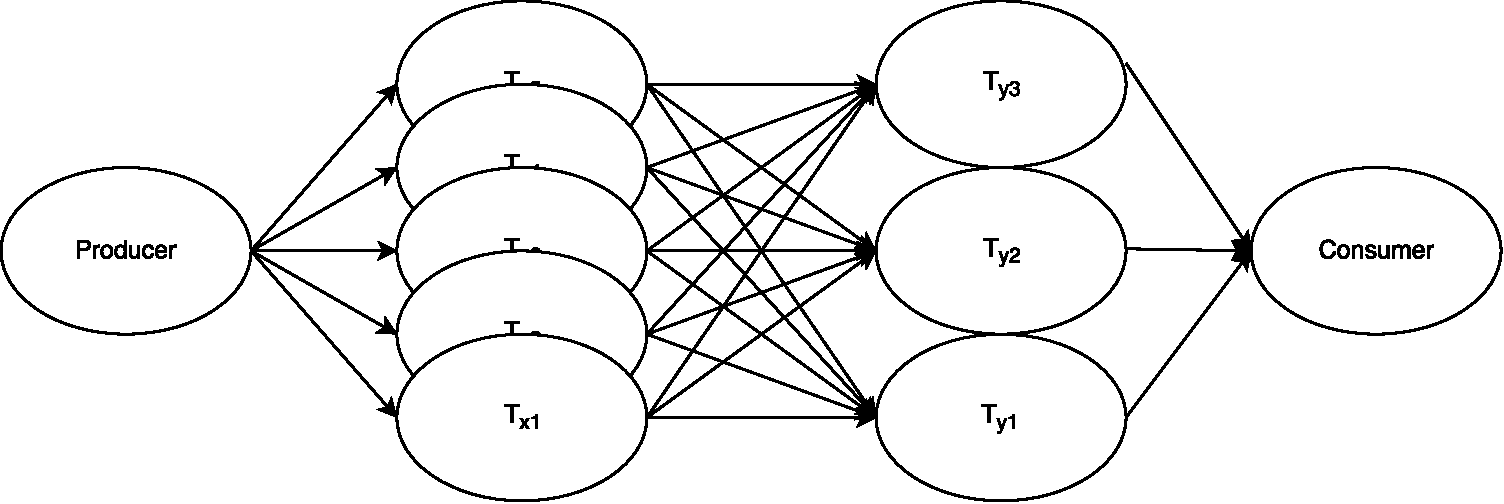
\includegraphics[scale=0.5]{images/extended_app_model_replication.pdf}
\caption{The data flow when two services, \emph{S1} and \emph{S2} with different required reliability are replicated.} \label[app]{fig:extended_app_model}
\end{figure}

\begin{figure}[!hbt]
\centering
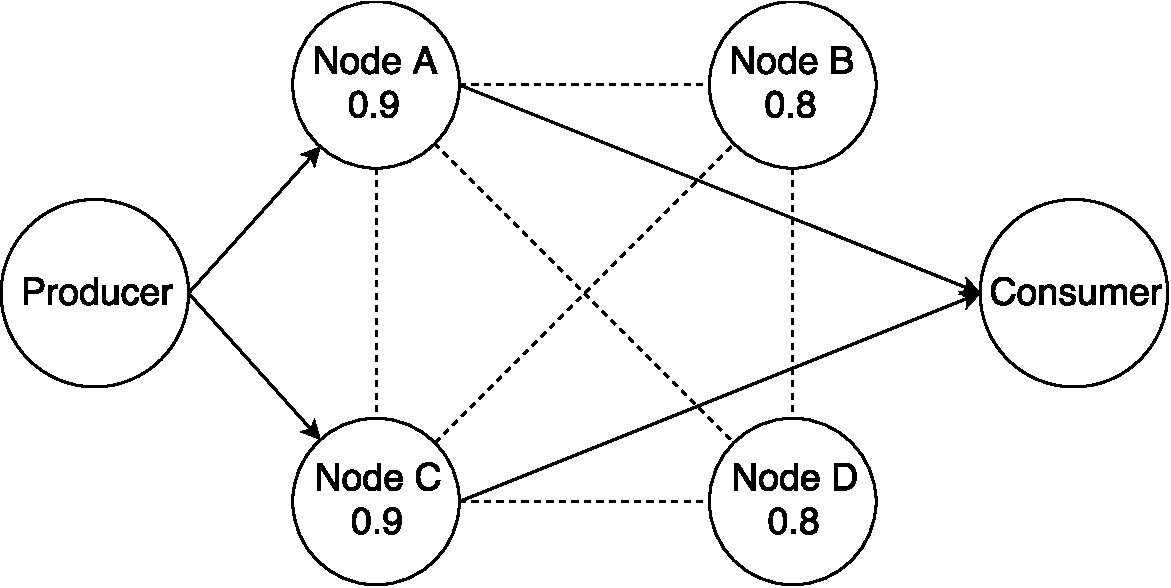
\includegraphics[scale=0.5]{images/before_node_failure.pdf}
\caption{Before a node failure. Here two replicas (placed on Node A and C) is required to achieve required reliability.} \label[app]{fig:before_node_failure}
\end{figure}

\begin{figure}[!hbt]
\centering
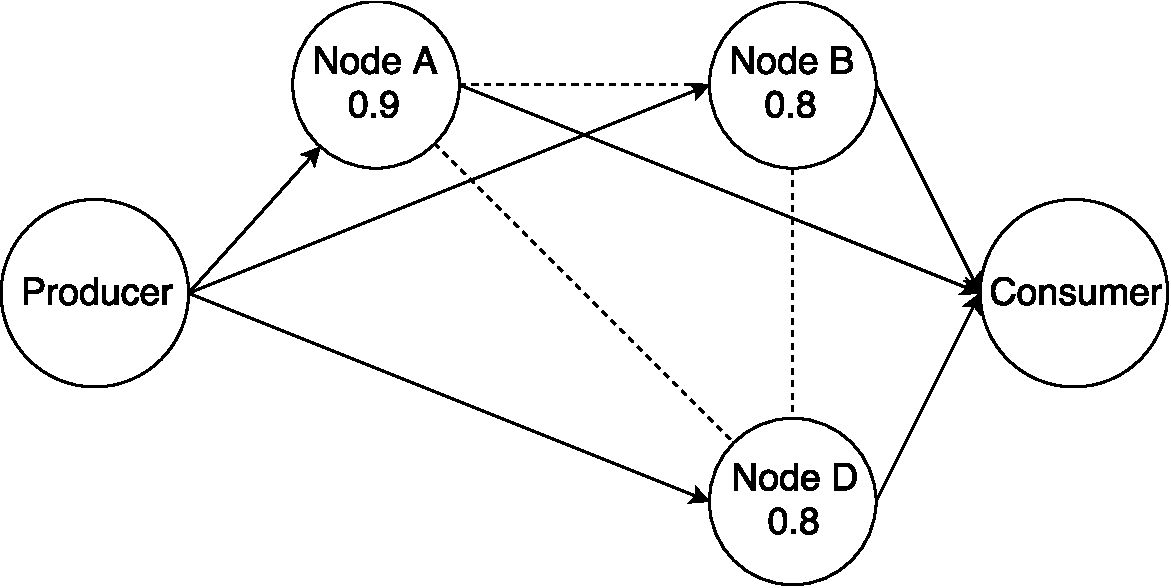
\includegraphics[scale=0.5]{images/after_node_failure.pdf}
\caption{After Node C has failed. Now three replicas (placed on Node A, B and D) is required to achieve required reliability.} \label[app]{fig:after_node_failure}
\end{figure}

%TODO change to exclude actors here as well? Or say that this is how it's done in Calvin.
\begin{figure}[!hbt]
\centering
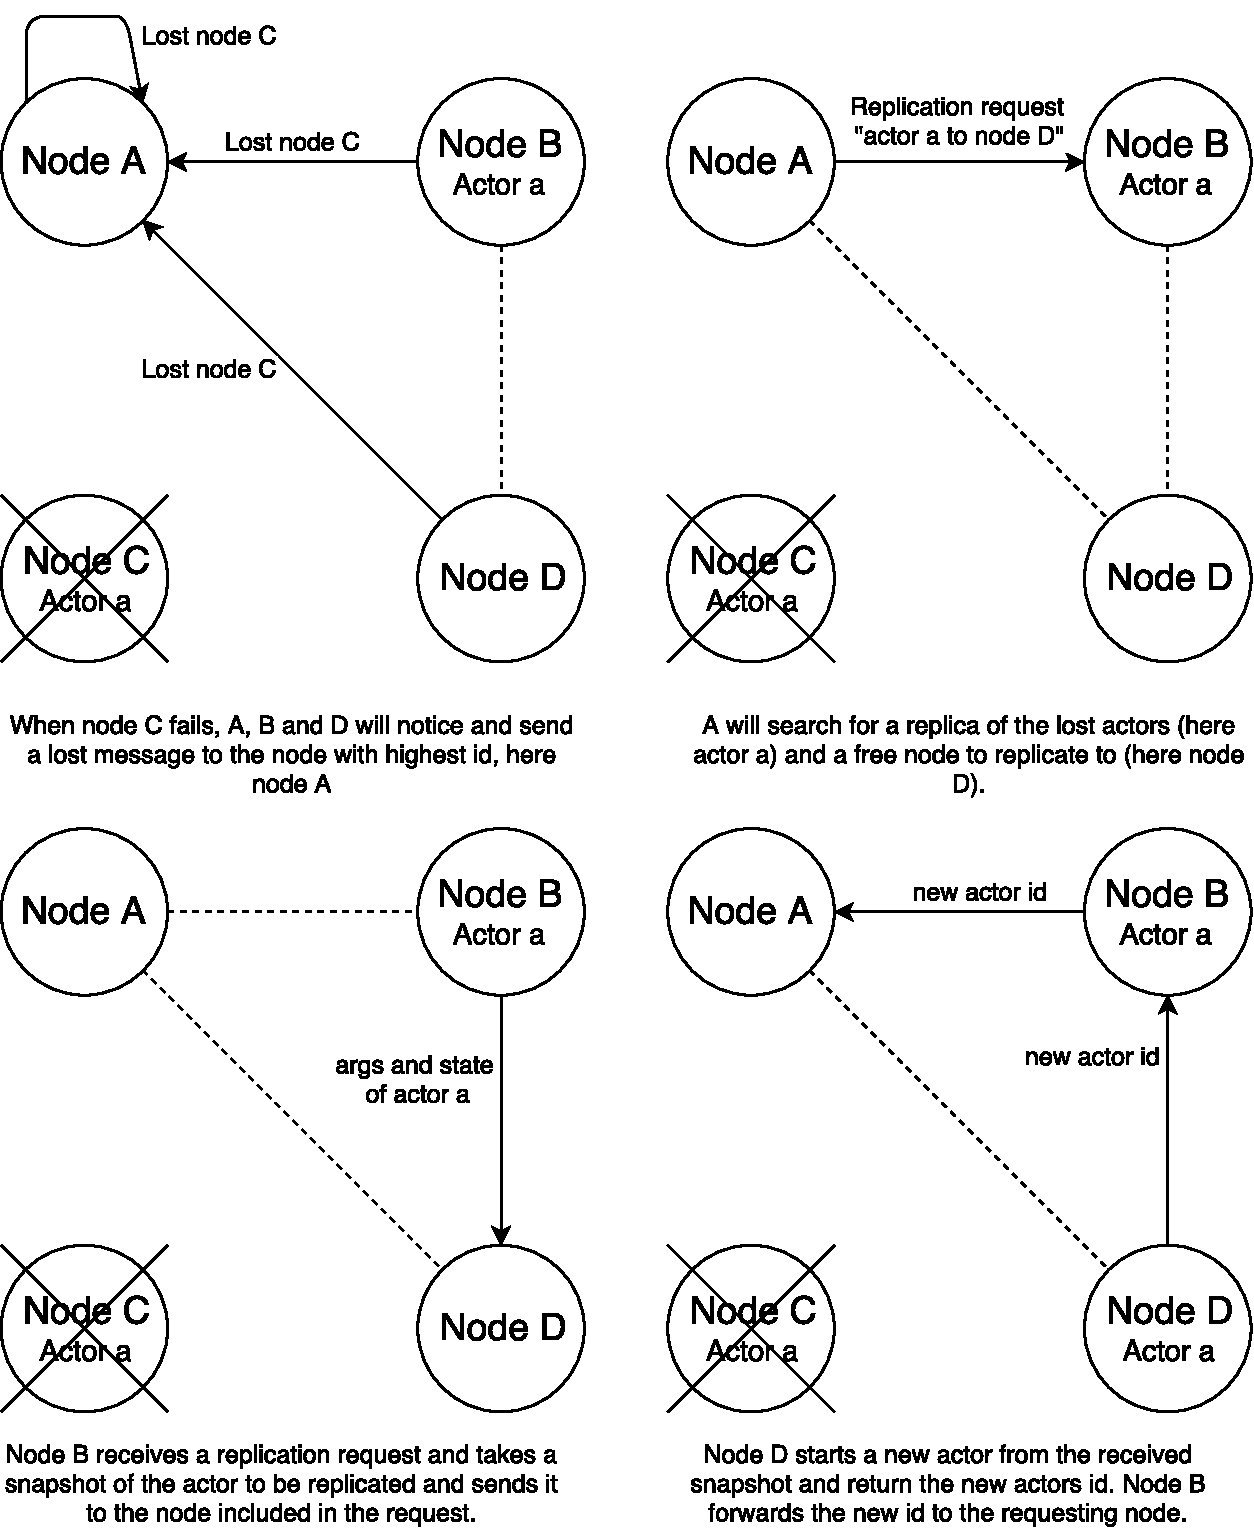
\includegraphics[scale=0.5]{images/replication_flow.pdf}
\caption{The most important parts of the communication after a node has failed.} \label[app]{fig:replication_flow}
\end{figure}

\begin{figure}[!hbt]
\centering
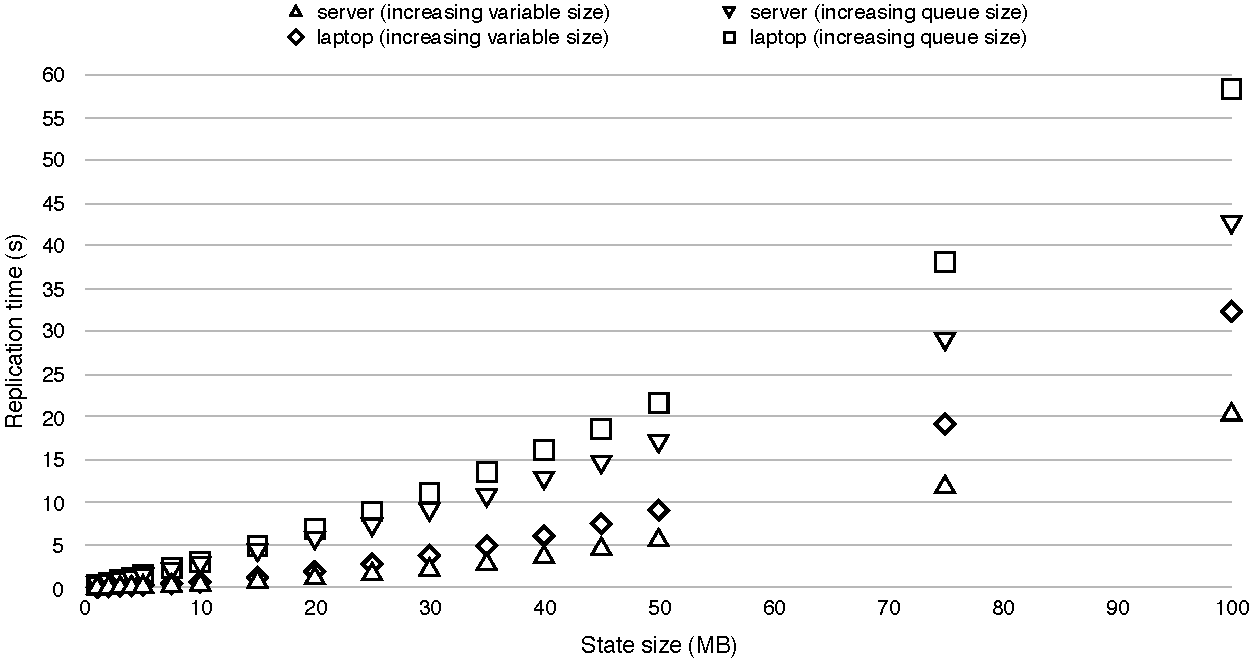
\includegraphics[scale=0.5]{images/results/replication_time/less_than_100.pdf} 
\caption{The average replication time as a function of state size.}\label[app]{fig:replication_time_less_than_100}
\end{figure}

\begin{figure}[!hbt]
\centering
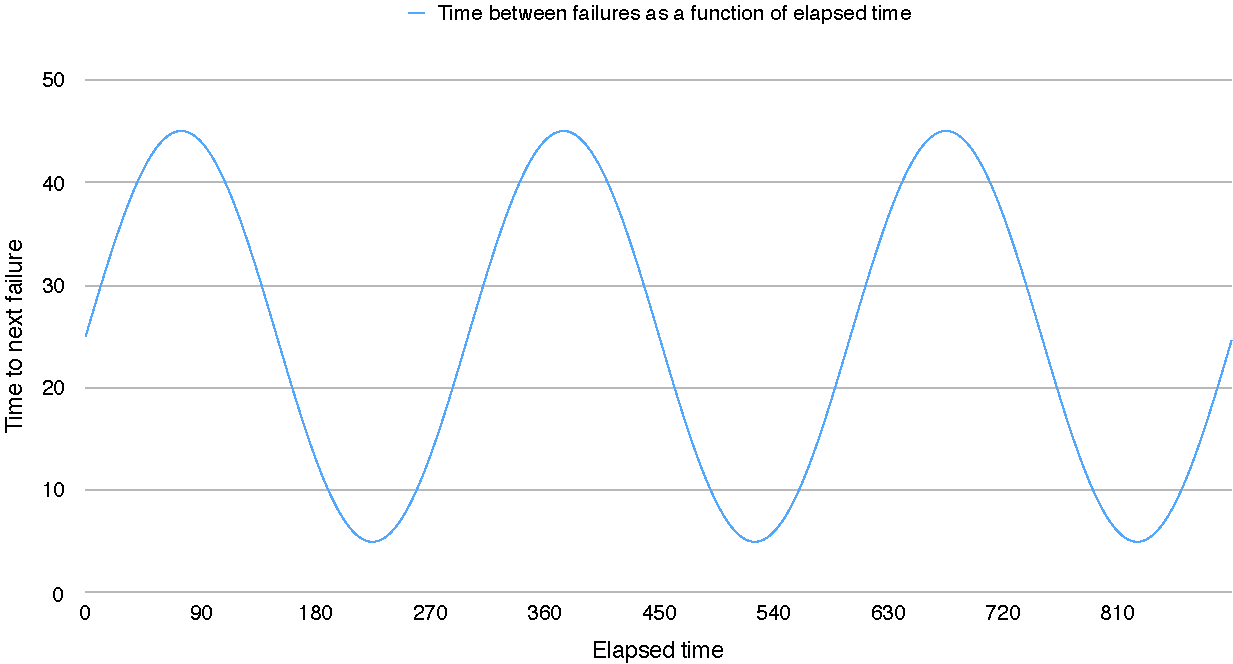
\includegraphics[scale=0.5]{images/sinus_failure_times.pdf}
\caption{Time between failures as of~\cref{eq:eval_sleep_time} used in test~\ref{sec:eval_adaptive_rel_model}.} \label[app]{fig:eval_sleep_time}
\end{figure}

\begin{figure}[!hbt]
\centering
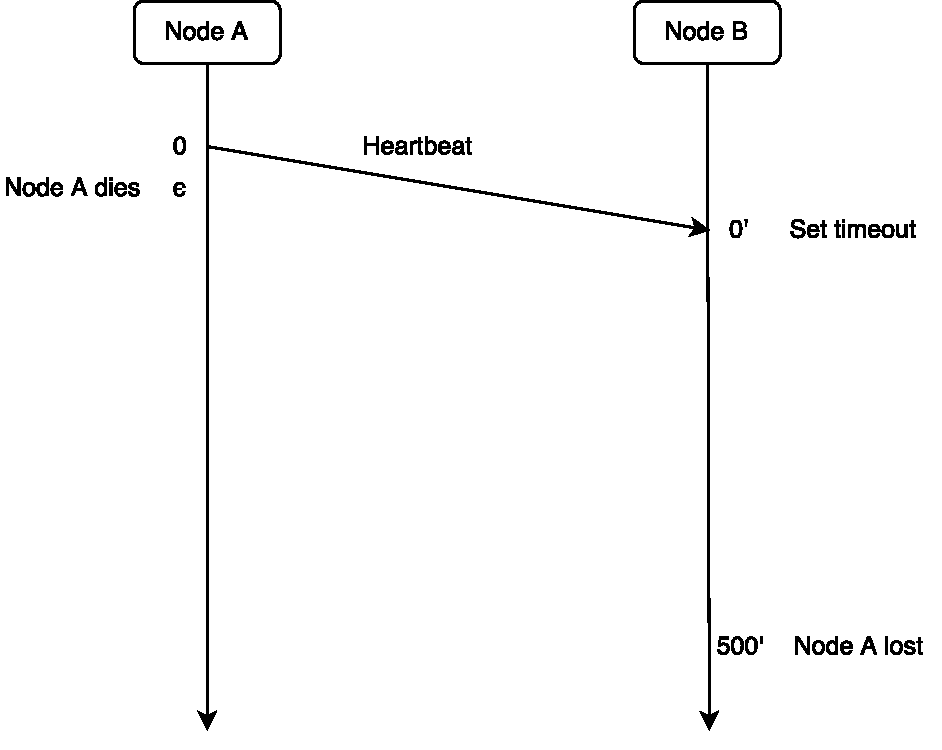
\includegraphics[scale=0.5]{images/heartbeats_worst_case.pdf}
\caption{Worst case scenario for detecting a failed node with $T_h$ set to 0.2 seconds, and $T_{timeout}$ to 0.5 seconds. In this example, node A fails directly after sending the heartbeat. The actual time node A has been dead before it's detected by node B is therefore close to 500 ms.} \label[app]{fig:heartbeats_worst_case}
\end{figure}

\begin{figure}[!hbt]
\centering
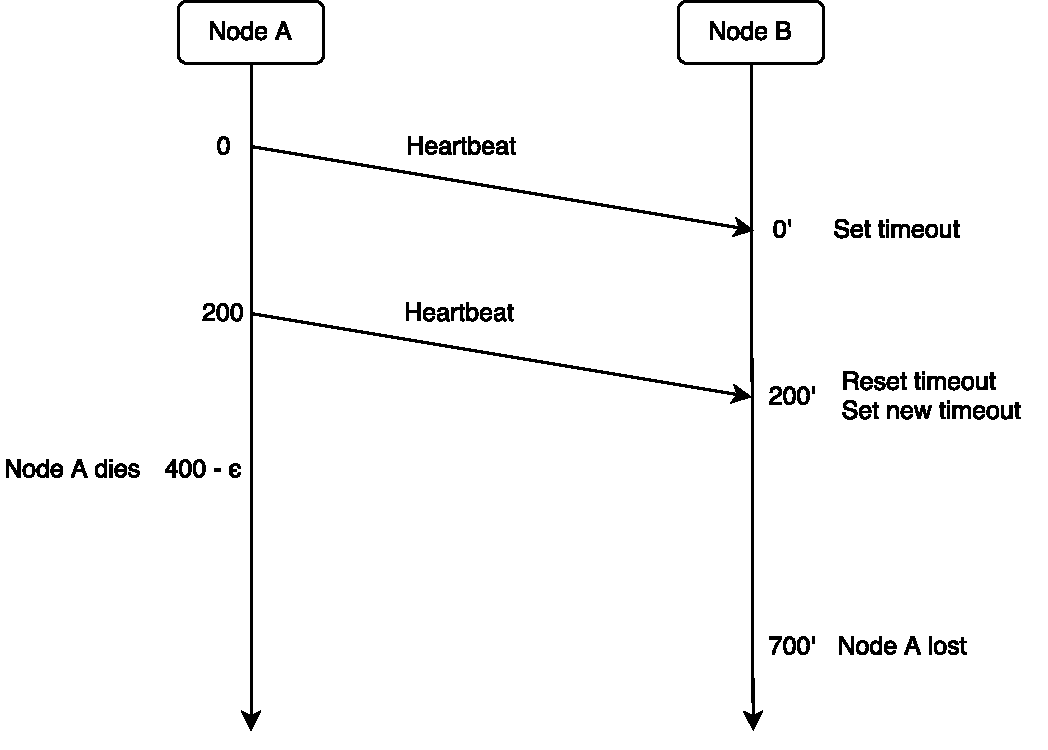
\includegraphics[scale=0.5]{images/heartbeats_best_case.pdf}
\caption{Best case scenario for detecting a failed node with $T_h$ set to 0.2 seconds, and $T_{timeout}$ to 0.5 seconds. In this example, node A fails just before sending the third heartbeat. The actual time node A has been dead before it's detected by node B is therefore close to 300 ms.} \label[app]{fig:heartbeats_best_case}
\end{figure}

\iffalse
\chapter{Code} \label{appendix:code}
\fi

\end{appendices}









\iffalse

% Below is the report template found online

\chapter[Short on Formatting]{Formatting}
Avoid empty spaces between \textit{chapter}-\textit{section}, \textit{section}-\textit{sub-section}. For instance, a very brief summary of the chapter would be one way of bridging the chapter heading and the first section of that chapter.
\section{Page Size and Margins}
Use A4 paper, with the text margins given in Table \ref{tab:margins}.
\begin{table}[!hbt]
\centering
\caption{Text margins for A4.}\label{tab:margins}
\begin{tabular}{cc}
\hline
\textbf{margin} & \textbf{space} \\
\hline 
top & 3.0cm\\ 

bottom & 3.0cm \\ 
 
left (inside) & 2.5cm \\ 

right (outside) & 2.5cm \\ 

binding offset & 1.0cm \\ 
\hline 
\end{tabular} 
\end{table}

\section{Typeface and Font Sizes}
The fonts to use for the reports are \textbf{TeX Gyre Termes} (a \textbf{Times New Roman} clone) for serif fonts, \textsf{\textbf{TeX Gyre Heros}} (a \textsf{\textbf{Helvetica}} clone) for sans-serif fonts, and finally \texttt{\textbf{TeX Gyre Cursor}} (a \texttt{\textbf{Courier}} clone) as mono-space font. All these fonts are included with the TeXLive 2013 installation. Table \ref{tab:fonts} lists the most important text elements and the associated fonts.
\begin{table}[!hbt]
\caption{Font types, faces and sizes to be used.}\label{tab:fonts}

 \begin{tabular}{ l c c c}
\hline 
\textbf{Element} & \textbf{Face} & \textbf{Size} & \textbf{\LaTeX size} \\ 
\hline 
{\huge \textbf{Ch. label}} & {\huge \textbf{serif, bold}} & \thefontsize\huge & \verb+\huge+ \\ 
{\Huge \textbf{Chapter}} & {\Huge \textbf{serif, bold}} & \thefontsize\Huge & \verb+\Huge+ \\ 
{\LARGE \textsf{\textbf{Section}}} & {\Large \textsf{\textbf{sans-serif, bold}}} & \thefontsize\LARGE & \verb+\LARGE+ \\ 
{\Large \textsf{\textbf{Subsection}}} & {\Large \textsf{\textbf{sans-serif, bold}}} & \thefontsize\Large & \verb+\Large+ \\ 
{\large \textsf{\textbf{Subsubsection}}} & {\Large \textsf{\textbf{sans-serif, bold}}} & \thefontsize\large & \verb+\large+ \\ 
Body & serif & \thefontsize\normalsize & {\footnotesize \verb+\normalsize+} \\
%{\footnotesize Footnote} & serif & \thefontsize\footnotesize & {\footnotesize \verb+\footnotesize+} \\
{\footnotesize \textsc{Header}} & {\footnotesize \textsc{serif, SmallCaps}} & \thefontsize\footnotesize & \\
Footer (page numbers) & serif, regular & \thefontsize\normalsize & \\
\hline
\textbf{Figure label} & \textbf{serif, bold} & \thefontsize\normalsize & \\
Figure caption & serif, regular & \thefontsize\normalsize & \\
\textsf{In figure} & \textsf{sans-serif} & \textit{any} & \\
\textbf{Table label} & \textbf{serif, bold} & \thefontsize\normalsize & \\
Table caption and text & serif, regular & \thefontsize\normalsize & \\
\texttt{Listings} & \texttt{mono-space} & $\le$ \thefontsize\normalsize & \\
\hline 
\end{tabular} 
\end{table}

\subsection{Headers and Footers}
Note that the page headers are aligned towards the outside of the page (right on the right-hand page, left on the left-hand page) and they contain the section title on the right and the chapter title on the left respectively, in \textsc{SmallCaps}. The footers contain only page numbers on the exterior of the page, aligned right or left depending on the page. The lines used to delimit the headers and footers from the rest of the page are $0.4 pt$ thick, and are as long as the text.

\subsection{Chapters, Sections, Paragraphs}
Chapter, section, subsection, etc. names are all left aligned, and numbered as in this document. 

Chapters always start on the right-hand page, with the label and title separated from the rest of the text by a $0.4 pt$ thick line.

Paragraphs are justified (left and right), using single line spacing. Note that the first paragraph of a chapter, section, etc. is not indented, while the following are indented.

\subsection{Tables}
Table captions should be located above the table, justified, and spaced 2.0cm from left and right (important for very long captions). Tables should be numbered, but the numbering is up to you, and could be, for instance:
\begin{itemize}
\item \textbf{Table X.Y} where X is the chapter number and Y is the table number within that chapter. (This is the default in \LaTeX. More on {\LaTeX} can be found on-line, including whole books, such as \cite{goossens93}.) or
\item \textbf{Table Y} where Y is the table number within the whole report
\end{itemize}
As a recommendation, use regular paragraph text in the tables, bold headings and avoid vertical lines (see Table \ref{tab:fonts}). 

\subsection{Figures}
Figure labels, numbering, and captions should be formed similarly to tables. As a recommendation, use vector graphics in figures (Figure \ref{fig:vectorg}), rather than bitmaps (Figure \ref{fig:rasterg}). Text within figures usually looks better with sans-serif fonts.
\begin{figure}[!hbt]
\centering

\includegraphics[scale=2.5]{images/examplepic1.pdf} 
\caption{A PDF vector graphics figure. Notice the numbering and placement of the caption. The caption text is indented 2.0cm from both left and right text margin.}\label{fig:vectorg}
\end{figure}

\begin{figure}[!hbt]
\centering

\includegraphics[scale=2.5]{images/examplepic3.jpg} 
\caption{A JPEG bitmap figure. Notice the bad quality of such an image when scaling it. Sometimes bitmap images are unavoidable, such as for screen dumps.}\label{fig:rasterg}
\end{figure}
For those interested in delving deeper into the design of graphical information display, please refer to books such as \cite{Tufte:1986, few2012show}.

\section{Mathematical Formulae and Equations}
You are free to use in-text equations and formulae, usually in \textit{italic serif} font. For instance: $S = \sum_i a_i$. We recommend using numbered equations when you do need to refer to the specific equations:
\begin{equation}
E = \int_0^{\delta} P(t) dt \quad \longleftrightarrow \quad E = m c^2
\end{equation}
The numbering system for equations should be similar to that used for tables and figures.

\section{References}
Your references should be gathered in a \textbf{References} section, located at the end of the document (before \textbf{Appendices}). We recommend using number style references, ordered as appearing in the document or alphabetically. Have a look at the references in this template in order to figure out the style, fonts and fields. Web references are acceptable (with restraint) as long as you specify the date you accessed the given link \cite{fontspec, CTAN}. You may of course use URLs directly in the document, using mono-space font, i.e. \url{http://cs.lth.se/}.

\section{Colours}
As a general rule, all theses are printed in black-and-white, with the exception of selected parts in selected theses that need to display colour images essential to describing the thesis outcome (\textit{computer graphics}, for instance).

A strong requirement is for using \textbf{black text on white background} in your document's main text. Otherwise we do encourage using colours in your figures, or other elements (i.e. the colour marking internal and external references) that would make the document more readable on screen. You may also emphasize table rows, columns, cells, or headers using white text on black background, or black text on light grey background.

Finally, note that the document should look good in black-and-white print. Colours are often rendered using monochrome textures in print, which makes them look different from on screen versions. This means that you should choose your colours wisely, and even opt for black-and-white textures when the distinction between colours is hard to make in print. The best way to check how your document looks, is to print out a copy yourself.

\chapter{Language}

You are strongly encouraged to write your report in English, for two reasons. First, it will improve your use of English language. Second, it will increase visibility for you, the author, as well as for the Department of Computer Science, and for your host company (if any).

However, note that your examiner (and supervisors) are not there to provide you with extensive language feedback. We recommend that you check the language used in your report in several ways:
\begin{description}
\item[Reference books] dedicated to language issues can be very useful. \cite{heffernan2000writing} 
\item[Spelling and grammar checkers] which are usually available in the commonly used text editing environments.
\item[Colleagues and friends] willing to provide feedback your writing.
\item[Studieverkstaden] is a university level workshop, that can help you with language related problems (see \href{http://www.lu.se/studera/livet-som-student/service-och-stod/studieverkstaden}{Studieverkstaden}'s web page).
\item[Websites] useful for detecting language errors or strange expressions, such as
\begin{itemize}
\item \url{http://translate.google.com}
\item \url{http://www.gingersoftware.com/grammarcheck/}
\end{itemize}
\end{description}

\section{Style Elements}
Next, we will just give some rough guidelines for good style in a report written in English. Your supervisor and examiner as well as the aforementioned \textbf{Studieverkstad} might have a different take on these, so we recommend you follow their advice whenever in doubt. If you want a reference to a short style guide, have a look at \cite{shortstyleguide}.

\subsubsection{Widows and Orphans}

Avoid \textit{widows} and \textit{orphans}, namely words or short lines at the beginning or end of a paragraph, which are left dangling at the top or bottom of a column, separated from the rest of the paragraph.

\subsubsection{Footnotes}

We strongly recommend you avoid footnotes. To quote from \cite{OGSW}, \textit{Footnotes are frequently misused by containing information which should either be placed in the text or excluded altogether. They should be avoided as a general rule and are acceptable only in exceptional cases when incorporation of their content in the text [is] not possible.} 

\subsubsection{Active vs. Passive Voice}

Generally active voice (\textit{I ate this apple.}) is easier to understand than passive voice (\textit{This apple has been eaten (by me).}) In passive voice sentences the actor carrying out the action is often forgotten, which makes the reader wonder who actually performed the action. In a report is important to be clear about who carried out the work. Therefore we recommend to use active voice, and preferably the plural form \textit{we} instead of \textit{I} (even in single author reports).

\subsubsection{Long and Short Sentences}
A nice brief list of sentence problems and solutions is given in \cite{yalesentences}. Using choppy sentences (too short) is a common problem of many students. The opposite, using too long sentences, occurs less often, in our experience.

\subsubsection{Subject-Predicate Agreement}
A common problem of native Swedish speakers is getting the subject-predicate (verb) agreement right in sentences. Note that a verb must agree in person and number with its subject. As a rough tip, if you have subject ending in \textit{s} (plural), the predicate should not, and the other way around. Hence, \textit{only one s}. Examples follow:
\begin{description}
\item[incorrect] He have to take this road.
\item[correct] He has to take this road.
\end{description}
\begin{description}
\item[incorrect] These words forms a sentence.
\item[correct] These words form a sentence.
\end{description}
\noindent In more complex sentences, getting the agreement right is trickier. A brief guide is given in the \textit{20 Rules of Subject Verb Agreement} \cite{subjectverb}.

\chapter{Structure}
It is a good idea to discuss the structure of the report with your supervisor rather early in your writing. Given next is a generic structure that is a starting point, but by no means the absolute standard. Your supervisor should provide a better structure for the specific field you are writing your thesis in. Note also that the naming of the chapters is not compulsory, but may be a helpful guideline.
\begin{description}
\item[Introduction] should give the background of your work. Important parts to cover:
\begin{itemize}
\item Give the context of your work, have a short introduction to the area.
\item Define the problem you are solving (or trying to solve).
\item Specify your contributions. What does this particular work/report bring to the research are or to the body of knowledge? How is the work divided between the co-authors? (This part is essential to pinpoint individual work. For theses with two authors, it is compulsory to identify which author has contributed with which part, both with respect to the work and the report.)
\item Describe related work (literature study). Besides listing other work in the area, mention how is it related or relevant to your work. The tradition in some research area is to place this part at the end of the report (check with your supervisor).
\end{itemize}
\item[Approach] should contain a description of your solution(s), with all the theoretical background needed. On occasion this is replaced by a subset or all of the following:
\begin{itemize}
\item \textbf{Method}: describe how you go about solving the problem you defined. Also how do you show/prove that your solution actually works, and how well does it work.
\item \textbf{Theory}: should contain the theoretical background needed to understand your work, if necessary.
\item \textbf{Implementation}: if your work involved building an artefact/implementation, give the details here. Note, that this should not, as a rule, be a chronological description of your efforts, but a view of the result. There is a place for insights and lamentation later on in the report, in the Discussion section.
\end{itemize}
\item[Evaluation] is the part where you present the finds. Depending on the area this part contains a subset or all of the following: 
\begin{itemize}
\item \textbf{Experimental Setup} should describe the details of the method used to evaluate your solution(s)/approach. Sometimes this is already addressed in the \textbf{Method}, sometimes this part replaces \textbf{Method}.
\item \textbf{Results} contains the data (as tables, graphs) obtained via experiments (benchmarking, polls, interviews).
\item \textbf{Discussion} allows for a longer discussion and interpretation of the results from the evaluation, including extrapolations and/or expected impact. This might also be a good place to describe your positive and negative experiences related to the work you carried out.
\end{itemize} 
Occasionally these sections are intermingled, if this allows for a better presentation of your work. However, try to distinguish between measurements or hard data (results) and extrapolations, interpretations, or speculations (discussion).
\item[Conclusions] should summarize your findings and possible improvements or recommendations.
\item[Bibliography] is a must in a scientific report. {\LaTeX} and \texttt{bibtex} offer great support for handling references and automatically generating bibliographies.
\item[Appendices] should contain lengthy details of the experimental setup, mathematical proofs, code download information, and shorter code snippets. Avoid longer code listings. Source code should rather be made available for download on a website or on-line repository of your choosing.

\end{description}
\makebibliography{MyMSc}

\begin{appendices}
\chapter{About This Document}
The following environments and tools were used to create this document:
\begin{itemize}
\item operating system: Mac OS X 10.10.1
\item tex distribution: MacTeX-2014, \url{http://www.tug.org/mactex/}
\item tex editor: Texmaker 4.4.1 for Mac, \url{http://www.xm1math.net/texmaker/} for its XeLaTeX flow (recommended) or pdfLaTeX flow
\item bibtex editor: BibDesk 1.6.3 for Mac, \url{http://bibdesk.sourceforge.net/}
\item fonts \texttt{cslthse-msc.cls} document class): 
\begin{description}
\item{for XeLaTeX}: TeX Gyre Termes, \textsf{TeX Gyre Heros}, \texttt{TeX Gyre Cursor} (installed from the TeXLive 2013)
\item{for pdfLaTeX}: TeX Gyre font packages: tgtermes.sty, tgheros.sty, tgcursor.sty, gtxmath.sty (available through TeXLive 2013) 
\end{description} 
\item picture editor: OmniGraffle Professional 5.4.2
\end{itemize}

\noindent A list of the essential \LaTeX packages needed to compile this document follows (all except \texttt{hyperref} are included in the document class):
\begin{itemize}
\item \texttt{fontspec}, to access local fonts, needs the XeLaTeX flow
\item \texttt{geometry}, for page layout
\item \texttt{titling}, for formatting the title page
\item \texttt{fancyhdr}, for custom headers and footers
\item \texttt{abstract}, for customizing the abstract
\item \texttt{titlesec}, for custom chapters, sections, etc.
\item \texttt{caption}, for custom tables and figure captions
\item \texttt{hyperref}, for producing PDF with hyperlinks
\item \texttt{appendix}, for appendices
\item \texttt{printlen}, for printing text sizes
\item \texttt{textcomp}, for text companion fonts (e.g. bullet)
\end{itemize}

\noindent Other useful packages:
\begin{itemize}
\item \texttt{listings}, for producing code listings with syntax colouring and line numbers
\end{itemize}

\chapter{List of Changes}
\subsubsection{Since 2015/04/27}
\begin{itemize}
\item Improved the \textbf{Structure} chapter and added more detailed comments for each part.
\end{itemize}

\subsubsection{Since 2014/02/18}
\begin{itemize}
\item Added the possibility to specify two supervisors. Use either of the \verb+\supervisor{}+ or \verb+\supervisors{}{}+ commands to set the names and contacts on the first page.
\end{itemize}

\subsubsection{Since 2013/09/23}
\begin{itemize}
\item Added missing colon ":" after \textit{Examiner} on the front page. 
\end{itemize}

\subsubsection{Since 2013/08/30}
\begin{itemize}
\item Changed fonts from Garamond (Times New Roman), Helvetica (Arial), Courier (Source Code Pro) to Tex Gyre fonts, namely Termes, Heros, Cursor, which are freely available with TexLive 2013 installation. These are all clones of Times New Roman, Helvetica and Courier, respectively. Garamond is problematic on some systems, being a non-freely available font.
\item Corrected the \textit{Face} column in Table \ref{tab:fonts} to correctly depict the font face.
\end{itemize}

\subsubsection{Since 2013/02/22}
\begin{itemize}
\item Number of words required in the abstract changed to 150 (from 300).
\end{itemize}

\subsubsection{Since 2013/02/15}
\begin{itemize}
\item Made a separate document class, for clarity.
\item made it work with pdfLaTeX and garamond.sty, in addition to XeLaTeX and true type fonts. It is up to the user to get the hold of the garamond.zip from \url{http://gael-varoquaux.info/computers/garamond/index.html}.
\end{itemize}
\end{appendices}

\fi

\end{document}
